% !TeX root = stable-vnmm2d.tex
%% 
%% Copyright 2007-2025 Elsevier Ltd
%% 
%% This file is part of the 'Elsarticle Bundle'.
%% ---------------------------------------------
%% 
%% It may be distributed under the conditions of the LaTeX Project Public
%% License, either version 1.3 of this license or (at your option) any
%% later version.  The latest version of this license is in
%%    http://www.latex-project.org/lppl.txt
%% and version 1.3 or later is part of all distributions of LaTeX
%% version 1999/12/01 or later.
%% 
%% The list of all files belonging to the 'Elsarticle Bundle' is
%% given in the file `manifest.txt'.
%% 
%% Template article for Elsevier's document class `elsarticle'
%% with numbered style bibliographic references
%% SP 2008/03/01
%% $Id: elsarticle-template-num.tex 272 2025-01-09 17:36:26Z rishi $
%%
\documentclass[preprint,12pt]{elsarticle}

%% Use the option review to obtain double line spacing
%% \documentclass[authoryear,preprint,review,12pt]{elsarticle}

%% Use the options 1p,twocolumn; 3p; 3p,twocolumn; 5p; or 5p,twocolumn
%% for a journal layout:
%% \documentclass[final,1p,times]{elsarticle}
%% \documentclass[final,1p,times,twocolumn]{elsarticle}
%% \documentclass[final,3p,times]{elsarticle}
%% \documentclass[final,3p,times,twocolumn]{elsarticle}
%% \documentclass[final,5p,times]{elsarticle}
%% \documentclass[final,5p,times,twocolumn]{elsarticle}

%% For including figures, graphicx.sty has been loaded in
%% elsarticle.cls. If you prefer to use the old commands
%% please give \usepackage{epsfig}

%% The amssymb package provides various useful mathematical symbols
\usepackage{amssymb}
%% The amsmath package provides various useful equation environments.
\usepackage{amsmath}
%% The amsthm package provides extended theorem environments
%% \usepackage{amsthm}
\usepackage{amsfonts}
%% The lineno packages adds line numbers. Start line numbering with
%% \begin{linenumbers}, end it with \end{linenumbers}. Or switch it on
%% for the whole article with \linenumbers.
%% \usepackage{lineno}
% --- Pacotes e Definição do Ambiente de Teoremas ---
\usepackage{amsthm}
\newtheorem{theorem}{Theorem}
\newtheorem{proposition}{Proposition}
\newtheorem{heuristic}{Heuristic}
\newtheorem{remark}{Remark}
\usepackage{graphicx}                 % Para inclusão de figuras
% Parâmetros para harmonizar posicionamento de figuras e evitar páginas exclusivas de flutuantes
\renewcommand{\topfraction}{0.88}
\renewcommand{\bottomfraction}{0.80}
\renewcommand{\textfraction}{0.12}
\renewcommand{\floatpagefraction}{0.75}
\usepackage{tabularx}
\usepackage{booktabs}                 % Para tabelas elegantes no padrão IEEE/Elsevier
\usepackage{bm}                       % Para notação de vetores em negrito
\usepackage{microtype}                % Melhora o espaçamento de palavras
\usepackage{float}                    % Controle preciso de posicionamento de figuras e tabelas [H], [!htbp]
\usepackage[pdfpagelabels=false]{hyperref} % Cria links ativos para equações e referências
\hypersetup{
    colorlinks=true,
    linkcolor=blue,
    citecolor=blue,
    urlcolor=blue,
    pdfencoding=auto,
    hypertexnames=false
}
\pdfstringdefDisableCommands{%
  \def\corref#1{}%
  \def\cnotenum#1{}%
}
\setlength{\emergencystretch}{2em}
\hbadness=3000

\journal{Engineering Analysis with Boundary Elements}

\begin{document}

\begin{frontmatter}

    %% Title, authors and addresses

    %% use the tnoteref command within \title for footnotes;
    %% use the tnotetext command for theassociated footnote;
    %% use the fnref command within \author or \affiliation for footnotes;
    %% use the fntext command for theassociated footnote;
    %% use the corref command within \author for corresponding author footnotes;
    %% use the cortext command for theassociated footnote;
    %% use the ead command for the email address,
    %% and the form \ead[url] for the home page:
    %% \title{Title\tnoteref{label1}}
    %% \tnotetext[label1]{}
    %% \author{Name\corref{cor1}\fnref{label2}}
    %% \ead{email address}
    %% \ead[url]{home page}
    %% \fntext[label2]{}
    %% \cortext[cor1]{}
    %% \affiliation{organization={},
    %%             addressline={},
    %%             city={},
    %%             postcode={},
    %%             state={},
    %%             country={}}
    %% \fntext[label3]{}

    % --- TÍTULO DO ARTIGO ---
    \title{A Stabilized Vector Nodal Meshless Method for \texorpdfstring{$H(\mathbf{curl})$}{H(curl)} 2D Electromagnetic Problems on Irregular Point Clouds}


    %% use optional labels to link authors explicitly to addresses:
    %% \author[label1,label2]{}
    %% \affiliation[label1]{organization={},
    %%             addressline={},
    %%             city={},
    %%             postcode={},
    %%             state={},
    %%             country={}}
    %%
    %% \affiliation[label2]{organization={},
    %%             addressline={},
    %%             city={},
    %%             postcode={},
    %%             state={},
    %%             country={}}

    \author[ufmg]{Renato C. Mesquita\corref{cor1}}
    \ead{renato@ufmg.br}
    \author[ufmg]{Elson J. da Silva}
    \author[ifetcongonhas]{Bárbara M. F. Gonçalves}
    \author[ifmgsabara]{Luilly A. G. Ortiz}

    \affiliation[ufmg]{organization={Department of Electrical Engineering, Universidade Federal de Minas Gerais},
        addressline={Av. Antônio Carlos, 6627},
        city={Belo Horizonte},
        postcode={31270-901},
        state={MG},
        country={Brazil}}

    \affiliation[ifetcongonhas]{organization={Mechanical Department, Instituto Federal de Educação, Ciência e Tecnologia de Minas Gerais, Campus Congonhas},
        addressline={Av. Michael Pereira de Souza, 3007},
        city={Congonhas},
        postcode={36417-050},
        state={MG},
        country={Brazil}}

    \affiliation[ifmgsabara]{organization={Industrial Control and Processes Department, Instituto Federal de Educação, Ciência e Tecnologia de Minas Gerais, Campus Sabará},
        addressline={Rodovia MGC-262, s/n, km 10},
        city={Sabará},
        postcode={34590-390},
        state={MG},
        country={Brazil}}

    \cortext[cor1]{Corresponding author}

    %% Abstract
    \begin{abstract}
        The Vector Nodal Meshless Method (VNMM) provides a node-based framework for $H(\mathbf{curl})$ vector-field approximation on point clouds. While early formulations relied on structured background subdivisions, extending the method to unconstrained point clouds reveals that the conventional incomplete solenoidal space ($\mathcal{L}^1$) triggers a persistent $\mathcal{O}(1)$ error plateau in curl approximation. This work resolves this limitation via a two-level framework addressing local polynomial consistency and global variational stability. Locally, $\mathcal{L}^1$ is replaced by the complete linear space $\mathcal{P}_1 \times \mathcal{P}_1$, capturing the full field Jacobian, eliminating derivative aliasing, and restoring observed first-order curl convergence without stagnation. Degenerate stencils are rejected through scale-aware determinant qualification on a dimensionless placement matrix $\widehat{\mathbf{A}}$ coupled with $k$-d tree searches. Globally, although VNMM exhibits exact constructive equivalence to lowest-order Whitney edge elements on conforming simplices, dynamic support stencils on unconstrained clouds destroy global trace conformity and discrete de Rham exactness, causing discrete gradient nullspace leakage in curl-curl eigenvalue formulations. We resolve this by incorporating a div-curl regularized Ritz-Galerkin formulation that shifts spurious modes away from the operational spectrum, leaving physical cavity resonances unperturbed. Numerical benchmarks demonstrate that integrating complete vector polynomials, scale-invariant support selection, and variational div-curl regularization offers an effective stabilized meshless framework exhibiting systematic convergence across the investigated regular and irregular point clouds. At the same time, the formulation currently relies on background cell-based integration (rather than a truly cell-free scheme) and achieves stability empirically for the tested regimes without explicit tangential-jump penalties, defining clear pathways for cell-free and discontinuous Galerkin extensions.
    \end{abstract}

    %% Graphical abstract (submitted separately as standalone image file to EABE)
    % \begin{graphicalabstract}
    % %\includegraphics{grabs}
    % \end{graphicalabstract}

    %% Research highlights (submitted separately as standalone file to EABE)
    % \begin{highlights}
    % \item Complete $\mathcal{P}^1$ basis overcomes curl stagnation of $\mathcal{L}^1$ VNMM.
    % \item Dimensionless matrix $\widehat{\mathbf{A}}$ prevents support dilation as $h \to 0$.
    % \item Local equivalence to Whitney 1-forms proved on conforming simplices.
    % \item Dynamic meshless supports induce global non-conformity in $H(\mathbf{curl})$.
    % \item Div-curl regularized weak form shifts spurious gradient modes outside the operational spectrum.
    % \end{highlights}

    %% Keywords
    \begin{keyword}
        %% keywords here, in the form: keyword \sep keyword
        Meshless methods \sep Vector Nodal Meshless Method (VNMM) \sep $H(\mathbf{curl})$ approximation \sep Spurious modes \sep Resonant cavities \sep Electromagnetics
        %% PACS codes here, in the form: \PACS code \sep code

        %% MSC codes here, in the form: \MSC code \sep code
        %% or \MSC[2008] code \sep code (2000 is the default)

    \end{keyword}

\end{frontmatter}

%% Add \usepackage{lineno} before \begin{document} and uncomment 
%% following line to enable line numbers
%% \linenumbers

%% main text
%%
% --- SEÇÃO 1: INTRODUÇÃO ---
\section{Introduction}
\label{sec:intro}

\subsection{Context and Motivation}
\label{subsec:context_motivation}

The numerical simulation of Maxwell's equations is central to modern computational electromagnetics (CEM) \cite{jin2014finite, harrington2001time, monk2003finite}. In CEM, discretizing Maxwell's equations via conventional node-based scalar Finite Element Methods (FEM) is well known to trigger severe pathologies \cite{jin2014finite, bossavit1998computational}: artificial locking of normal discontinuities across material boundaries, inaccurate modeling of edge singularities, and spectral pollution by non-physical spurious modes resulting from the violation of the discrete de Rham complex ($\operatorname{Im}(\nabla) \not\subset \ker(\nabla \times)$) \cite{bossavit1990spurious, boffi1999computational, boffi2013mixed}. Although N\'ed\'elec's edge finite elements (EFEM/Whitney forms) \cite{nedelec1980mixed, monk2003finite} resolve these issues by natively conforming in $H(\mathbf{curl}; \Omega)$, they require high-quality conforming meshes. For complex CAD geometries, moving parts in electrical machinery, and adaptive refinement, mesh generation and distortion repair represent severe computational bottlenecks \cite{idelsohn2006mesh, liu2009mesh, slak2018refined}.

To circumvent mesh constraints, meshless methods construct approximations of the electric field $\vec{E}$ directly on unstructured point clouds \cite{liu2009mesh, belytschko1994element}. Early adaptations based on scalar Moving Least Squares (EFG) or local Petrov-Galerkin schemes (MLPG) \cite{viana1999moving, cingoski1998element, atluri2002meshless, fonseca2008imposing, nicomedes2012meshless} approximated Cartesian components ($E_x, E_y$) independently. Because such approximations artificially enforce $C^0$ continuity on all vector components across material boundaries, they re-introduced spectral pollution and tangential locking unless augmented by costly divergence-free projections or Lagrange multipliers \cite{nicomedes2015mixed, lima2016metodos}.

The Point Interpolation Method (PIM) developed by Liu and Gu \cite{liu2001point} established a purely interpolating framework: by inverting a local moment matrix of size matching the polynomial basis dimension, PIM constructs shape functions that satisfy the Kronecker delta property, allowing exact and straightforward imposition of essential boundary conditions. However, PIM was also conceived as an inherently scalar formulation.

To provide native vector regularity in computational electromagnetics while retaining the interpolating capability of PIM, Lima and Mesquita introduced the Edge Meshless Method (EMM) \cite{lima2017edge}, subsequently equipped by Silva et al. \cite{silva2018new} with N\'ed\'elec-type $\mathcal{L}^1$ vector shape functions. Rather than interpolating scalar point values, the EMM adapted the interpolating philosophy of PIM to vector fields by formulating the interpolation over the circuital line integral of the vector field along a finite edge segment:
\begin{equation}
    e_k = \int_{L_k} \vec{E} \cdot d\boldsymbol{\ell}.
    \label{eq:emm_circulation_dof}
\end{equation}
By taking the asymptotic limit as physical edge lengths contract to point-collocated nodes ($L_k \to 0$ with $d\boldsymbol{\ell} \to \vec{t}_k dl$), Ortiz et al. \cite{ortiz2021creating, ortiz2021nodal, ortiz2023tese} established the Vector Nodal Meshless Method (VNMM), later extended to 3D and periodic problems \cite{goncalves2023vector, goncalves2025tese, goncalves2026periodic}.

In this continuous-to-nodal limit, the VNMM inherits the interpolating character of PIM: its vector shape functions satisfy the Kronecker delta property with respect to the discrete degrees of freedom, but what is now interpolated is the local directional projection of the vector field along the node's unit vector director:
\begin{equation}
    e_i = \vec{E}(P_i) \cdot \vec{t}_i.
    \label{eq:vnmm_projection_dof}
\end{equation}
In the VNMM, the 1D continuous edge is therefore replaced by a vector node $(P_i, \vec{t}_i)$ endowed with a unit director $\vec{t}_i$ \cite{ortiz2021nodal, ortiz2023tese}. Assigning a single directional projection degree of freedom ($e_i$) per node directly overcomes the fundamental limitation of component-wise vector meshless methods: instead of allocating two independent degrees of freedom ($E_x, E_y$) per node and artificially locking normal jumps across interfaces, the VNMM preserves single-DoF scalar efficiency while aligning boundary and interface directors tangentially. This enables direct nodal collocation of tangential continuity and essential PEC boundary conditions ($e_i = 0$), while permitting natural, unconstrained jumps in the normal component across material interfaces without Lagrange multipliers \cite{ortiz2021nodal, goncalves2025tese}. Table~\ref{tab:meshless_comparison} compares conventional CEM discretizations with the stabilized VNMM developed herein.

\begin{table}[!htbp]
    \centering
    \footnotesize
    \renewcommand{\arraystretch}{0.92}
    \setlength{\tabcolsep}{3pt}
    \caption{Conceptual comparison of spatial discretization paradigms in computational electromagnetics.}
    \label{tab:meshless_comparison}
    \begin{tabularx}{\linewidth}{@{}
        >{\raggedright\arraybackslash}p{0.17\linewidth}
        >{\centering\arraybackslash}p{0.13\linewidth}
        >{\centering\arraybackslash}p{0.16\linewidth}
        >{\centering\arraybackslash}p{0.14\linewidth}
        >{\centering\arraybackslash}p{0.18\linewidth}
        >{\centering\arraybackslash}X
        @{}}
        \toprule
        \textbf{Method}                                                                      &
        \textbf{Mesh Req.}                                                                   &
        \textbf{DoF Type}                                                                    &
        \textbf{$H(\mathbf{curl})$ Trace}                                                    &
        \textbf{Spurious Control}                                                            &
        \textbf{Point-Cloud Curl Rate}                                                         \\
        \midrule
        \textbf{Edge FEM (EFEM)} \cite{nedelec1980mixed, monk2003finite, boffi2013mixed}     &
        Conformal mesh                                                                       &
        Edge circulation $\int_{E_k} \vec{E} \cdot d\boldsymbol{\ell}$                       &
        Natively conforming ($\mathbf{n} \times [\vec{E}] = \mathbf{0}$)                     &
        Exact discrete de Rham complex                                                       &
        $\mathcal{O}(h^1)$ (simplex-based)                                                     \\
        \addlinespace
        \textbf{Scalar EFG / MLS} \cite{belytschko1994element, cingoski1998element}          &
        None (Cloud)                                                                         &
        Component splitting ($E_x, E_y$)                                                     &
        Artificial ($C^0$ normal locking / penalty)                                          &
        Divergence penalty                                                                   &
        $\mathcal{O}(h^p)$ (high-order MLS)                                                    \\
        \addlinespace
        \textbf{Vector MLPG} \cite{atluri2002meshless, nicomedes2012meshless}                &
        None (Local subdomains)                                                              &
        Component splitting ($E_x, E_y$)                                                     &
        Lagrange multipliers / penalty                                                       &
        Divergence-free projection                                                           &
        $\mathcal{O}(h^p)$ (local MLS integration)                                             \\
        \addlinespace
        \textbf{Scalar PIM / RPIM} \cite{liu2001point, liu2005introduction, slak2018refined} &
        None (Cloud)                                                                         &
        Component splitting ($E_x, E_y$)                                                     &
        Collocation / ghost penalty                                                          &
        Divergence cleaning / penalty                                                        &
        $\mathcal{O}(h^p)$ (polynomial/radial interpolation)                                   \\
        \addlinespace
        \textbf{Original VNMM ($\mathcal{L}^1$)} \cite{ortiz2021nodal, ortiz2023tese}        &
        Planar / Delaunay subdivision                                                        &
        Projection $e_k = \vec{E}(P_k) \cdot \vec{t}_k$                                      &
        Natural tangential alignment                                                         &
        Conditional (structured supports)                                                    &
        $\mathcal{O}(h^1)$ on meshes; $\mathcal{O}(1)$ plateau on clouds                       \\
        \addlinespace
        \textbf{Proposed VNMM ($\mathcal{P}^1$)}                                             &
        None (Arbitrary point clouds)                                                        &
        Projection $e_k = \vec{E}(P_k) \cdot \vec{t}_k$                                      &
        Natural tangential alignment                                                         &
        Divergence penalty                                                                   &
        $\mathcal{O}(h^1)$ expected \newline (obs. $p \in [0.75, 0.97]$)                      \\
        \bottomrule
    \end{tabularx}
\end{table}

\subsection{Local and Global Bottlenecks on Unconstrained Point Clouds: Curl Stagnation, Stencil Degeneracy, and Spectral Pollution}
\label{subsec:curl_stagnation_bottleneck}

Despite the mathematical elegance of the original VNMM \cite{ortiz2021nodal, ortiz2023tese}, early formulations achieved convergence by relying on structured support selections (e.g., macro-element subdivisions or Delaunay triangulations), where closed-contour circulation cancellation prevented curl error stagnation. However, reliance on underlying meshes undermines the core meshless premise of unconstrained point-cloud discretization \cite{liu2009mesh, goncalves2025tese}.

Under automated stencil selection ($k$-d tree queries) on unconstrained point clouds, the incomplete solenoidal basis $\mathcal{L}^1$ breaks down: \textbf{the numerical curl $(\nabla \times \vec{E}^h)_z$ fails to converge, exhibiting an $\mathcal{O}(1)$ error plateau under spatial refinement} (Section~\ref{subsec:L1_aliasing_analysis}). Unlike conforming edge elements where Stokes' theorem guarantees boundary circulation cancellation \cite{nedelec1980mixed, monk2003finite}, point collocation lacks closed-contour integration. In $\mathcal{L}^1$, omitting dilatational gradients ($\partial E_x/\partial x$, $\partial E_y/\partial y$) prevents shape functions from capturing the complete first-order variation; on arbitrary clouds, unrepresented modes contaminate the rotational degree of freedom, producing persistent modal aliasing.

Additionally, because the VNMM inherits the interpolating framework of PIM, shape functions are constructed by inverting a square placement matrix $\mathbf{A}$ matching the basis dimension ($3 \times 3$ for $\mathcal{L}^1$, $6 \times 6$ for $\mathcal{P}^1$). Consequently, like the moment matrices in classic scalar PIM \cite{liu2001point}, arbitrary clouds and directors can generate geometrically degenerate stencils where $\det(\mathbf{A}) \to 0$, corrupting matrix conditioning.

Furthermore, dynamic support stencils render the global meshless space non-conforming ($V_h \not\subset H(\mathbf{curl}; \Omega)$), breaking discrete de Rham exactness and leaking gradient nullspaces into the non-zero spectrum as spurious modes. Stabilizing the VNMM on unconstrained clouds therefore requires a two-level approach: completing the local polynomial basis ($\mathcal{L}^1 \to \mathcal{P}^1$) to resolve the local Jacobian, and employing a div-curl regularized Ritz-Galerkin weak formulation to restore global spectral purity (Section~\ref{sec:variational_formulation}).

\subsection{Scope and Main Contributions of the Paper}
\label{subsec:scope_contributions}

This paper presents a stabilized Vector Nodal Meshless Method (VNMM) for robust vector field approximations on unconstrained point clouds without mesh connectivity. The core methodological contributions are fourfold:

\begin{enumerate}
    \item \textbf{Elimination of Modal Aliasing and Linear Patch-Test Consistency via $\mathcal{P}^1$:}
          Adopting the complete linear space $\mathcal{P}^1 = \mathcal{P}_1 \times \mathcal{P}_1$ resolves all four components of the field Jacobian $\mathbf{J}^h = \nabla \vec{E}^h$ (Section~\ref{subsec:complete_P1_basis}), eliminating the derivative aliasing responsible for curl stagnation in $\mathcal{L}^1$. Furthermore, it satisfies the Galerkin patch test to machine precision ($\le 7.4 \times 10^{-14}$) across all affine vector modes---confirming linear completeness of the discrete operator---and delivers systematic asymptotic convergence ($\mathcal{O}(h^{2.08})$ in $L^2$ and $\mathcal{O}(h^{0.75})$ in $H(\mathbf{curl})$) for driven source problems via the Method of Manufactured Solutions (MMS), whereas $\mathcal{L}^1$ exhibits errors up to $47\%$ and complete convergence stagnation (Section~\ref{subsec:patch_test_galerkin}).

    \item \textbf{Scale-Invariant Support Selection via Dimensionless Placement Matrix $\widehat{\mathbf{A}}$:}
          To enable stable mesh-free operation on unstructured clouds, we characterize matrix singularity in $\mathbb{R}^{6\times6}$ via the Null-Space Orthogonality Principle (Section~\ref{subsec:singularities_P1}) and eliminate the quartic scaling $\det(\mathbf{A}) \sim \mathcal{O}(h^4)$ by introducing a dimensionless placement matrix $\widehat{\mathbf{A}}$. Normalizing local stencils by the spacing $h_{\mathrm{local}}$ decouples qualification ($|\det(\widehat{\mathbf{A}})| \ge \widehat{\mathrm{Tol}} > 0$) from physical dimensions, preserving compact locality without support dilation as $h \to 0$ (Section~\ref{sec:conditioning}).

    \item \textbf{Rigorous Local Constructive Equivalence Proof:}
          We establish the Local Dual Equivalence Theorem (Section~\ref{subsubsec:formal_proof_dual_whitney}), proving that under conforming midpoint/tangent placement, local VNMM $\mathcal{L}^1$ shape functions and lowest-order Whitney 1-forms are constructively identical. This result clarifies the fundamental distinction between mesh-conforming topologies, where shared cell facets guarantee global $H(\mathbf{curl})$ conformity, and unconstrained point clouds, where dynamically shifting stencils inevitably induce global non-conformity.

    \item \textbf{Variational Div-Curl Regularization for Non-Conforming Meshless Discretizations:}
          To address gradient leakage stemming from global non-conformity ($V_h \not\subset H(\mathbf{curl}; \Omega)$), we formulate a div-curl regularized Ritz-Galerkin weak formulation ($\mathbf{K} = \mathbf{K}_{\mathrm{curl}} + s_{\mathrm{div}} \mathbf{K}_{\mathrm{div}}$, Section~\ref{sec:variational_formulation}), reliably shifting non-physical gradient modes outside the operational bandwidth without auxiliary Lagrange multipliers or saddle-point indefiniteness.
\end{enumerate}

The remainder of this paper is organized as follows: Section~\ref{sec:formulations} formulates the VNMM shape functions for the $\mathcal{L}^1$ and $\mathcal{P}^1$ bases and proves the Local Dual Equivalence Theorem; Section~\ref{sec:conditioning} analyzes placement singularities and develops scale-invariant support selection; Section~\ref{sec:variational_formulation} establishes the div-curl regularized weak form; Section~\ref{sec:numerical_results} presents numerical verification (patch test, MMS, cavity spectra, and irregular clouds); and Section~\ref{sec:conclusion} concludes the paper.

% --- SEÇÃO 2: FORMULAÇÃO MATEMÁTICA ---
\section{Mathematical Formulations of the 2D VNMM}
\label{sec:formulations}

This section establishes the functional framework of the two-dimensional Vector Nodal Meshless Method (VNMM 2D). We define the single-DoF nodal projection scheme and pointwise boundary conditions, analyze the topological equivalence between the classical $\mathcal{L}^1$ basis and Whitney 1-forms on conforming simplices, and formulate the complete linear vector space $\mathcal{P}^1$ to resolve the local field Jacobian and eliminate derivative aliasing.

\subsection{Nodal Projection and Tangential Continuity}
\label{subsec:nodal_projection}

The VNMM \cite{ortiz2021nodal, ortiz2023tese} constructs local $H(\mathbf{curl})$-regular vector approximations by distributing a set of $M$ nodes throughout the computational domain $\Omega$ and its boundaries $\partial\Omega$. Unlike traditional scalar meshless formulations that assign separate degrees of freedom to individual spatial components (e.g., $E_x$ and $E_y$), the VNMM associates a single physical unit vector director $\vec{t}_i = [t_{ix}, t_{iy}]^T$ with each node $i$.

The approximate vector field $\vec{E}^h(\mathbf{x})$ at any spatial location $\mathbf{x} = (x, y) \in \Omega$ is expressed as a linear combination of vector nodal shape functions $\vec{N}_i(\mathbf{x})$:
\begin{equation}
    \vec{E}^h(x, y) = \sum_{i=1}^{M_{\text{supp}}} \vec{N}_i(x, y) e_i
    \label{eq:field_approx_vnmm}
\end{equation}
where $M_{\text{supp}}$ is the number of active support nodes in the local influence domain, and $e_i$ represents the discrete scalar degree of freedom (DoF) associated with the $i$-th node. Physically, $e_i$ corresponds to the pointwise directional projection of the electric field vector along the unit vector director $\vec{t}_i$ at the node coordinate $\mathbf{x}_i = (x_i, y_i)$:
\begin{equation}
    e_i = \vec{E}(\mathbf{x}_i) \cdot \vec{t}_i \quad [\text{Volts/meter}]
    \label{eq:dof_projection_definition}
\end{equation}

To ensure physical consistency, local curl regularity, and direct enforcement of boundary conditions, the vector shape functions $\vec{N}_i(\mathbf{x})$ are required to satisfy the vector Kronecker delta projection property \cite{lima2017edge, ortiz2021nodal}:
\begin{equation}
    \vec{N}_i(\mathbf{x}_k) \cdot \vec{t}_k = \delta_{ik} = \begin{cases} 1, & \text{if } k = i \\ 0, & \text{if } k \neq i \end{cases}
    \label{eq:vector_kronecker_delta}
\end{equation}
for all nodes $k$ belonging to the local support domain. Property~\eqref{eq:vector_kronecker_delta} dictates that the shape function $\vec{N}_i$ exhibits a unit projection along its own nodal director $\vec{t}_i$ at position $\mathbf{x}_i$, while maintaining zero projection along the directors of all other surrounding support nodes.

\subsubsection{Enforcement of PEC Boundary Conditions and Remarks on Material Interfaces}
The vector Kronecker delta property~\eqref{eq:vector_kronecker_delta} enables a direct, unconstrained nodal collocation of essential Dirichlet boundary conditions and tangential field continuity without requiring background auxiliary meshes, penalty parameters, or Lagrange multipliers \cite{goncalves2023vector, ortiz2021nodal}.

For nodes lying on Perfect Electric Conductor (PEC) boundaries $\Gamma_{\text{PEC}}$, where the physical boundary condition requires $\hat{n} \times \vec{E} = \mathbf{0}$ ($\hat{n}$ being the outward unit normal to $\partial\Omega$), the associated vector director $\vec{t}_k$ is aligned tangent to the boundary contour:
\begin{equation}
    \vec{t}_k \parallel \partial\Omega \implies \hat{n}(\mathbf{x}_k) \cdot \vec{t}_k = 0.
\end{equation}
Consequently, setting the scalar nodal degree of freedom directly to zero:
\begin{equation}
    e_k = 0 \quad \forall \mathbf{x}_k \in \Gamma_{\text{PEC}}
    \label{eq:pec_dirichlet_homog}
\end{equation}
enforces the PEC requirement pointwise at every boundary node:
\begin{equation}
    \vec{E}^h(\mathbf{x}_k) \cdot \vec{t}_k = 0 \quad \forall \mathbf{x}_k \in \Gamma_{\text{PEC}},
    \label{eq:pec_nodal_collocation}
\end{equation}
by virtue of the vector Kronecker delta property~\eqref{eq:vector_kronecker_delta}.

\paragraph{Nodal Collocation versus Continuous Boundary Trace}
From a functional analysis viewpoint, the pointwise nodal collocation condition~\eqref{eq:pec_nodal_collocation} must be distinguished from the continuous functional trace condition:
\begin{equation}
    \hat{n} \times \vec{E}^h = \mathbf{0} \quad \text{everywhere on } \Gamma_{\text{PEC}}.
    \label{eq:pec_continuous_trace}
\end{equation}
On conforming simplicial triangulations (Section~\ref{subsubsec:formal_proof_dual_whitney}), internal DoFs have identically vanishing tangential traces along boundary edges, so the nodal constraint~\eqref{eq:pec_nodal_collocation} guarantees that Eq.~\eqref{eq:pec_continuous_trace} holds everywhere along $\Gamma_{\text{PEC}}$. On unconstrained point clouds, however, the global approximation is non-conforming ($V_h \not\subset H(\mathbf{curl}; \Omega)$). For points $\mathbf{x} \in \Gamma_{\text{PEC}}$ between nodes, dynamic stencils $\mathcal{S}(\mathbf{x})$ include interior nodes with $e_i \neq 0$ whose shape functions do not vanish tangentially along $\partial\Omega$. Setting $e_k = 0$ enforces the PEC condition at boundary nodes $\mathbf{x}_k$, while continuous trace satisfaction is variational. Similarly, on curved boundaries with tangent directors $\vec{t}_k = \hat{\tau}(\mathbf{x}_k)$, the condition is collocated directly without polygonization, while the trace between nodes converges under spatial refinement.

\paragraph{Material Interfaces and Homogeneous Scope}
Assigning unit directors tangent to material interfaces $\Gamma_{\text{int}}$ ($\vec{t}_i = \hat{\tau}(\mathbf{x}_i)$) enables direct collocation of tangential continuity ($\vec{E}^h_1 \cdot \vec{t}_i = \vec{E}^h_2 \cdot \vec{t}_i = e_i$) while permitting the normal field to undergo a physical step discontinuity ($E_{n1} \neq E_{n2}$), avoiding the normal locking of scalar $C^0$ meshless schemes. Normal flux continuity ($D_{n1} = D_{n2} \iff \epsilon_{r1} E_{n1} = \epsilon_{r2} E_{n2}$) is enforced variationally by the weak form and divergence penalty. Rigorous handling of heterogeneous media requires partitioned support stencils (e.g., multi-tree $k$-d trees \cite{parreira2006efficient}) to prevent unphysical gradient smoothing across subdomains; because this work focuses on homogeneous benchmarks ($\epsilon_r = 1, \mu_r = 1$), systematic treatment of heterogeneous interfaces is deferred to future work (Section~\ref{subsec:future_works}).

\subsection{The Incomplete \texorpdfstring{$\mathcal{L}^1$}{L1} Basis (3 Support Nodes)}
\label{subsec:incomplete_l1_basis}
The construction of vector shape functions in the 2D VNMM directly inherits the mathematical foundations of $H(\mathbf{curl})$-conforming edge-based meshless approximations \cite{lima2017edge, silva2018new}. The incomplete 3-term solenoidal polynomial space
\begin{equation}
    \mathcal{L}^1 = \operatorname{span}\{ \begin{bmatrix}1\\0\end{bmatrix}, \begin{bmatrix}0\\1\end{bmatrix}, \begin{bmatrix}y\\-x\end{bmatrix} \}
\end{equation}
corresponds to the local two-dimensional reduction of Nédélec's first-type space \cite{nedelec1980mixed}, whose vector projection mechanisms were established for edge meshless line segments by Silva et al. \cite{silva2018new} and later adapted to point-collocated nodes \cite{ortiz2021nodal, ortiz2023tese}.

Consequently, the local vector shape function $\vec{N}_i$ associated with the $i$-th support node in a 3-node local domain is defined as a linear combination of these basis vectors:
\begin{equation}
    \vec{N}_i(x, y) = \beta_{1i} \begin{bmatrix} 1 \\ 0 \end{bmatrix} + \beta_{2i} \begin{bmatrix} 0 \\ 1 \end{bmatrix} + \beta_{3i} \begin{bmatrix} y \\ -x \end{bmatrix}
    \label{eq:N_i_L1}
\end{equation}
where $\boldsymbol{\beta}_i = [\beta_{1i}, \beta_{2i}, \beta_{3i}]^T \in \mathbb{R}^3$ represents the unknown local interpolation coefficient vector.

To determine these coefficients, the vector shape functions are constrained to satisfy the vector Kronecker delta projection property~\eqref{eq:vector_kronecker_delta} for $i,k=1,2,3$,

Applying constraint~\eqref{eq:vector_kronecker_delta} to all three support nodes leads to the local $3 \times 3$ linear placement system:
\begin{equation}
    \mathbf{A} \boldsymbol{\beta}_i = \mathbf{L}_i
    \label{eq:linear_placement_system}
\end{equation}
where the local moment placement matrix $\mathbf{A} \in \mathbb{R}^{3 \times 3}$ is explicitly given by:
\begin{equation}
    \mathbf{A} = \begin{bmatrix}
        t_{1x} & t_{1y} & y_1 t_{1x} - x_1 t_{1y} \\
        t_{2x} & t_{2y} & y_2 t_{2x} - x_2 t_{2y} \\
        t_{3x} & t_{3y} & y_3 t_{3x} - x_3 t_{3y}
    \end{bmatrix}
    \label{eq:matrix_A_L1}
\end{equation}
and the canonical load vectors are $\mathbf{L}_1 = [1, 0, 0]^T$, $\mathbf{L}_2 = [0,1,0]^T$, and $\mathbf{L}_3 = [0,0,1]^T$.

Once the coefficients $\boldsymbol{\beta}_i = \mathbf{A}^{-1} \mathbf{L}_i$ are evaluated, the approximated electric field vector $\vec{E}^h(x, y)$ is constructed via nodal projection superposition:
\begin{equation}
    \vec{E}^h(x, y) = \sum_{i=1}^3 \vec{N}_i(x, y) e_i
\end{equation}
where $e_i = \vec{E}(\mathbf{x}_i) \cdot \vec{t}_i$ represent the discrete scalar projection DoFs.

\subsubsection{Mathematical Properties}
The shape functions $\vec{N}_i$ of the $\mathcal{L}^1$ basis possess two distinct mathematical characteristics:

1. \textbf{Identical Solenoidal Property ($\nabla \cdot \vec{N}_i \equiv 0$):} Taking the divergence of Eq.~\eqref{eq:N_i_L1} yields:
\begin{equation}
    \nabla \cdot \vec{N}_i = \frac{\partial}{\partial x}(\beta_{1i} + \beta_{3i} y) + \frac{\partial}{\partial y}(\beta_{2i} - \beta_{3i} x) \equiv 0
\end{equation}

2. \textbf{Univariate Curl Representation:} Evaluating the scalar $z$-directed curl operator on $\vec{N}_i$ yields:
\begin{equation}
    (\nabla \times \vec{N}_i)_z = \frac{\partial N_{iy}}{\partial x} - \frac{\partial N_{ix}}{\partial y} = \frac{\partial (-\beta_{3i} x)}{\partial x} - \frac{\partial (\beta_{3i} y)}{\partial y} = -2\beta_{3i}
\end{equation}
Therefore, the approximated $z$-directed scalar curl field $(\nabla \times \vec{E}^h)_z$ is spatially constant across the 3-node support domain and depends exclusively on the third coefficient $\beta_{3i}$:
\begin{equation}
    (\nabla \times \vec{E}^h)_z = -2 \sum_{i=1}^3 \beta_{3i} e_i
\end{equation}

\subsubsection{Local Constructive Equivalence under Conforming Midpoint/Tangent Placement}
\label{subsubsec:dual_whitney}
The VNMM 2D was originally conceptualized as the zero-edge-length asymptotic limit of the Edge Meshless Method (EMM) \cite{lima2017edge, ortiz2021nodal}. By examining this heritage, a fundamental local constructive equivalence under conforming midpoint/tangent placement between the VNMM point-collocation formulation and classic lowest-order Whitney edge finite elements (N\'ed\'elec 1-forms on triangular simplices \cite{nedelec1980mixed, monk2003finite, boffi2013mixed}) is formally established, as detailed in Fig.~\ref{fig:whitney_vnmm_dual_equivalence}.

\begin{figure*}[!t]
    \centering
    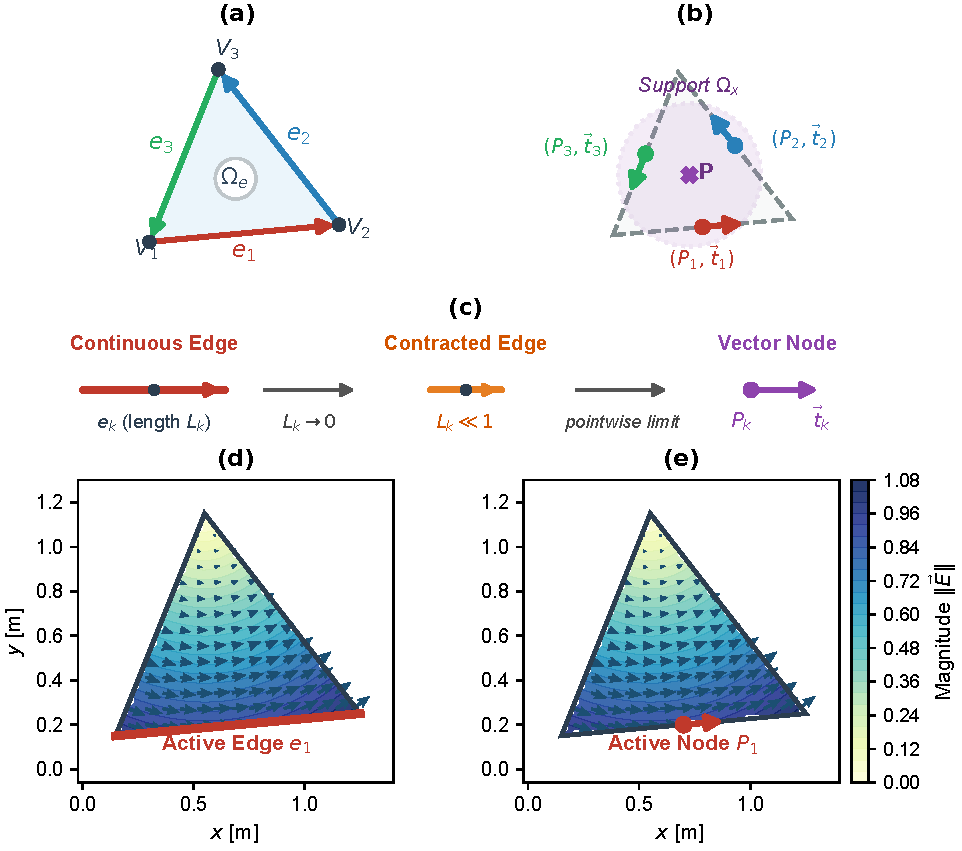
\includegraphics[width=\textwidth]{figura_equivalencia_dual_whitney_vnmm.pdf}
    \caption{Local equivalence between Whitney edge elements and the VNMM $\mathcal{L}^1$ basis.
        (a) Triangular cell $\Omega_e$ with vertices $V_i$ and oriented edges $e_k$;
        (b) VNMM support stencil with vector nodes $(P_k, \vec{t}_k)$ placed at edge midpoints;
        (c) Asymptotic collapse ($L_k \to 0$) mapping edge circulations to directional projections $e_k$;
        (d) Whitney 1-form $\vec{w}_1$ for edge $e_1$;
        (e) Normalized VNMM basis $\vec{N}_1/L_1$ for node $(P_1, \vec{t}_1)$, displaying identical vector fields over $\Omega_e$.}
    \label{fig:whitney_vnmm_dual_equivalence}
\end{figure*}


In conventional FEM (Fig.~\ref{fig:whitney_vnmm_dual_equivalence}a), the degrees of freedom associated with the triangular cell $\Omega_e$ are line integrals of circulation $\alpha_k = \oint_{e_k} \vec{E} \cdot d\boldsymbol{\ell}$ along continuous 1D edges of finite physical length $L_k$. As demonstrated in the asymptotic collapse limit (Fig.~\ref{fig:whitney_vnmm_dual_equivalence}c), when the physical edge length shrinks to zero ($L_k \to 0$), the 1D continuous edge degenerates into a point-collocated vector node $(P_k, \vec{t}_k)$, where the circulation DoF $\alpha_k$ naturally scales into a pointwise directional field projection $e_k = \vec{E}(P_k) \cdot \vec{t}_k$ [Volts/meter].

\subsubsection{The Local Dual Equivalence Theorem}
\label{subsubsec:formal_proof_dual_whitney}
Let $T \subset \mathbb{R}^2$ be an arbitrary non-degenerate triangular simplex with vertices $V_1, V_2, V_3$ ordered counter-clockwise and non-zero area $|T| > 0$. Let $e_k = (V_k, V_{k+1})$ be the directed boundary edges of length $L_k = \|V_{k+1} - V_k\| > 0$, with unit tangent vectors $\vec{t}_k = (V_{k+1} - V_k)/L_k$ and midpoints $M_k = \frac{1}{2}(V_k + V_{k+1})$ for $k \in \{1, 2, 3\}$ (with index wrap-around $V_4 \equiv V_1$).

\begin{theorem}[Local Constructive Equivalence under Conforming Midpoint/Tangent Placement]
    \label{thm:dual_equivalence}
    Consider the support triad of vector nodes $\{P_k, \vec{t}_k\}_{k=1}^3$ defined at the edge midpoints $P_k = M_k$ with directors $\vec{t}_k$. The VNMM 2D $\mathcal{L}^1$ shape functions $\vec{N}_k(\mathbf{x})$ and the Whitney 1-forms $\vec{w}_k(\mathbf{x}) = \lambda_i(\mathbf{x})\nabla\lambda_j - \lambda_j(\mathbf{x})\nabla\lambda_i$ (with $(i,j)=(k,k+1)$) satisfy:
    \begin{equation}
        \vec{N}_k(\mathbf{x}) \equiv L_k \, \vec{w}_k(\mathbf{x}) \quad \Longleftrightarrow \quad \vec{w}_k(\mathbf{x}) \equiv \frac{1}{L_k} \vec{N}_k(\mathbf{x}), \quad \forall \mathbf{x} \in \mathbb{R}^2, \ \forall k \in \{1, 2, 3\}
        \label{eq:dual_equivalence_scaling}
    \end{equation}
\end{theorem}

\begin{proof}[Outline of Proof]
    The constructive equivalence follows from two geometric and algebraic properties: (i) both the Whitney 1-form space $\mathcal{W}(T)$ and the VNMM $\mathcal{L}^1$ basis span identical 3-dimensional vector polynomial spaces; and (ii) the tangential projection $\vec{u}(\mathbf{x}) \cdot \vec{t}_k$ of any affine field $\vec{u} \in \mathcal{L}^1$ is invariant along each edge $e_k$. Consequently, boundary circulation integrals reduce to midpoint evaluations scaled by the edge length, $\oint_{e_k} \vec{u} \cdot d\boldsymbol{\ell} = L_k (\vec{u}(M_k) \cdot \vec{t}_k)$, establishing an exact unisolvent isomorphism between Whitney circulations and VNMM point-collocated directional projections ($\vec{N}_k \equiv L_k \vec{w}_k$). The complete five-step constructive proof is provided in \ref{app:dual_whitney_proof}.
\end{proof}

As graphically illustrated in Fig.~\ref{fig:whitney_vnmm_dual_equivalence}d and~\ref{fig:whitney_vnmm_dual_equivalence}e (and verified numerically in Section~\ref{subsec:conforming_dual_equivalence}), the normalized VNMM $\mathcal{L}^1$ shape functions $\frac{1}{L_k}\vec{N}_k$ and canonical Whitney 1-forms $\vec{w}_k$ match identically across the simplex $T$ down to floating-point machine precision ($\approx 10^{-16}$).

\subsubsection{Local \texorpdfstring{$H(\mathbf{curl})$}{H(curl)} Regularity versus Global \texorpdfstring{$H(\mathbf{curl})$}{H(curl)} Conformity}
Beyond establishing the mathematical connection to edge finite elements, this constructive identity clarifies a fundamental structural distinction in vector meshless approximations:
\begin{enumerate}
    \item \textbf{Local $H(\mathbf{curl})$ Regularity on Virtual Simplices:} In conventional scalar meshless methods (e.g., Moving Least Squares or Element-Free Galerkin), evaluating field approximations outside the physical convex hull enclosed by the node coordinates $\mathbf{x}_k$ constitutes an unconstrained extrapolation, leading to rapid truncation error growth \cite{lima2017edge}. In contrast, because the VNMM vector basis reproduces the complete polynomial space of Whitney edge elements over the virtual macro-triangle $\Omega_{x}$ defined by the intersecting lines of action of vector directors $\vec{t}_k$ (Fig.~\ref{fig:whitney_vnmm_dual_equivalence}b), the valid domain for local $H(\mathbf{curl})$ field approximation is not geographically restricted to the small physical convex hull of $\mathbf{x}_k$ \cite{nedelec1980mixed, monk2003finite}. Under regular-support assumptions (well-conditioned local placement matrix $\mathbf{A}$ and non-degenerate intersection vertices), any field evaluation at $P \in \Omega_{x}$ preserves local $H(\mathbf{curl})$ regularity.
    \item \textbf{Loss of Global $H(\mathbf{curl})$ Conformity on Unconstrained Point Clouds:} When nodes and directors form a conforming simplicial mesh (Section~\ref{subsubsec:formal_proof_dual_whitney}), tangential traces across adjacent element facets match identically, yielding global conformity $V_h \subset H(\mathbf{curl}; \Omega)$. On unconstrained point clouds, however, dynamically shifting support stencils induce inter-stencil tangential trace discontinuities, rendering the global approximation non-conforming ($V_h \not\subset H(\mathbf{curl}; \Omega)$). The spectral consequences of this global non-conformity and its variational stabilization are addressed in Section~\ref{sec:variational_formulation}.
\end{enumerate}

\subsubsection{Mathematical Origin of Modal Aliasing and Curl Stagnation}
\label{subsec:L1_aliasing_analysis}

While the incomplete solenoidal basis $\mathcal{L}^1$ exhibits exact dual equivalence to Whitney elements on conforming meshes (Section~\ref{subsubsec:dual_whitney}), its behavior diverges sharply on unconstrained point clouds, where curl approximations stagnate at an $\mathcal{O}(1)$ relative error plateau under spatial refinement (as numerically confirmed in Section~\ref{subsubsec:curl_stagnation_L1} and Fig.~\ref{fig:convergencia_interpolacao_L1_vs_P1}b). To uncover the algebraic origin of this derivative stagnation, we examine the local Taylor series expansion of the exact electric field $\vec{E}$ centered at an evaluation point $P(x_P, y_P)$ \cite{li2007meshfree, liu2009mesh}:
\begin{equation}
    \vec{E}(\mathbf{x}) = \vec{E}(P) + \mathbf{J}(P) \begin{bmatrix} \Delta x \\[2pt] \Delta y \end{bmatrix} + \mathcal{O}(h^2)
    \label{eq:taylor_vector_expansion}
\end{equation}
where $\mathbf{J}(P) = \nabla \vec{E}$ represents the complete first-order field Jacobian tensor \cite{liu2009mesh}:
\begin{equation}
    \mathbf{J} = \begin{bmatrix}
        \frac{\partial E_x}{\partial x} & \frac{\partial E_x}{\partial y} \\[4pt]
        \frac{\partial E_y}{\partial x} & \frac{\partial E_y}{\partial y}
    \end{bmatrix}
    \label{eq:jacobian_tensor_raw}
\end{equation}

By expressing individual spatial derivatives in terms of fundamental vector calculus operators---namely, the field divergence $\nabla \cdot \vec{E} = \partial E_x/\partial x + \partial E_y/\partial y$ and the z-directed field curl $(\nabla \times \vec{E})_z = \partial E_y/\partial x - \partial E_x/\partial y$---the field Jacobian tensor is decomposed as:
\begin{equation}
    \mathbf{J} = \frac{1}{2}(\nabla \cdot \vec{E}) \mathbf{I} + \frac{1}{2}(\nabla \times \vec{E})_z \begin{bmatrix} 0 & -1 \\ 1 & 0 \end{bmatrix} + \begin{bmatrix} \delta_{\mathrm{norm}} & \delta_{\mathrm{trans}} \\ \delta_{\mathrm{trans}} & -\delta_{\mathrm{norm}} \end{bmatrix} \equiv \mathbf{J}_{\mathrm{div}} + \mathbf{J}_{\mathrm{rot}} + \mathbf{J}_{\mathrm{shear}}
    \label{eq:jacobian_tensor_EM_decomposition}
\end{equation}
where the three matrix terms represent, respectively: (i) the \textbf{isotropic dilation (divergence) matrix} $\mathbf{J}_{\mathrm{div}} = \frac{1}{2}(\nabla \cdot \vec{E}) \mathbf{I}$, with $\mathbf{I} \in \mathbb{R}^{2 \times 2}$ being the identity matrix; (ii) the \textbf{skew-symmetric rotational (curl) matrix} $\mathbf{J}_{\mathrm{rot}} = \frac{1}{2}(\nabla \times \vec{E})_z \begin{bmatrix} 0 & -1 \\ 1 & 0 \end{bmatrix}$; and (iii) the \textbf{symmetric trace-free shear (deviatoric) matrix} $\mathbf{J}_{\mathrm{shear}} = \begin{bmatrix} \delta_{\mathrm{norm}} & \delta_{\mathrm{trans}} \\ \delta_{\mathrm{trans}} & -\delta_{\mathrm{norm}} \end{bmatrix}$ (satisfying $\operatorname{tr}(\mathbf{J}_{\mathrm{shear}}) = 0$). Here, $\delta_{\mathrm{norm}} = \frac{1}{2}(\partial E_x/\partial x - \partial E_y/\partial y)$ denotes the normal (longitudinal) field derivative difference, and $\delta_{\mathrm{trans}} = \frac{1}{2}(\partial E_y/\partial x + \partial E_x/\partial y)$ represents the symmetric transverse (shear) field derivative component.

In the incomplete $\mathcal{L}^1$ basis, local shape functions provide only 3 degrees of freedom. As a result, normal field derivatives are artificially forced to vanish identically ($\partial E_x^h/\partial x \equiv 0$ and $\partial E_y^h/\partial y \equiv 0$), imposing $\nabla \cdot \vec{E}^h \equiv 0$, $\delta_{\mathrm{norm}} \equiv 0$, and $\delta_{\mathrm{trans}} \equiv 0$ simultaneously.

This fundamental limitation is captured by the following order-of-magnitude scaling heuristic:

\begin{heuristic}[Jacobian Incompleteness and Derivative Modal Aliasing Scaling]
    \label{heur:L1_aliasing}
    Let $\vec{E} \in [C^2(\Omega)]^2$ be an arbitrary twice continuously differentiable 2D vector field. The incomplete solenoidal space $\mathcal{L}^1 = \operatorname{span}\{[1, 0]^T, [0, 1]^T, [y, -x]^T\} \subset \mathcal{P}_1 \times \mathcal{P}_1$ cannot reproduce the complete first-order Taylor expansion of $\vec{E}$. Specifically, while the complete space $\mathcal{P}^1 = \mathcal{P}_1 \times \mathcal{P}_1$ possesses $\dim(\mathcal{P}^1) = 6$ degrees of freedom to reconstruct the 2 translation components and all 4 independent entries of the Jacobian tensor $\mathbf{J} = \nabla\vec{E}$, $\mathcal{L}^1$ possesses only $\dim(\mathcal{L}^1) = 3$ degrees of freedom, enforcing the artificial linear constraints:
    \begin{equation}
        \frac{\partial E_x^h}{\partial x} = 0, \quad \frac{\partial E_y^h}{\partial y} = 0, \quad \text{and} \quad \frac{\partial E_x^h}{\partial y} + \frac{\partial E_y^h}{\partial x} = 0.
        \label{eq:L1_derivative_constraints}
    \end{equation}
    On unconstrained point clouds lacking conforming circulation cancellation, projecting the unrepresented Jacobian components onto the 3-node stencil induces a residual $\|\mathbf{r}\| \sim \mathcal{O}(h)$ which, under the $\mathcal{O}(h^{-1})$ scaling of the rotational row of $\mathbf{A}^{-1}$, produces an $\mathcal{O}(1)$ derivative aliasing error:
    \begin{equation}
        |(\nabla \times \vec{E})_z - (\nabla \times \vec{E}^h)_z| \sim \|\operatorname{Row}_3(\mathbf{A}^{-1})\| \|\mathbf{r}\| = \mathcal{O}(h^{-1}) \cdot \mathcal{O}(h) = \mathcal{O}(1).
        \label{eq:aliasing_order_proof}
    \end{equation}
\end{heuristic}

The algebraic derivation of this scaling estimate is detailed in \ref{app:heuristic_aliasing_proof}.

\begin{remark}[Scope of Heuristic~\ref{heur:L1_aliasing} and the Conforming Case]
    \label{rem:heur1_scope}
    The estimate in Heuristic~\ref{heur:L1_aliasing} is an order-of-magnitude scaling heuristic, attained when the weights of $\operatorname{Row}_3(\mathbf{A}^{-1})$ fail to annihilate the unrepresented symmetric component $\mathbf{S} = \mathbf{J}_{\mathrm{div}} + \mathbf{J}_{\mathrm{shear}} = \frac{1}{2}(\mathbf{J} + \mathbf{J}^T)$ of the Jacobian tensor. In the conforming midpoint/tangent configuration of Theorem~\ref{thm:dual_equivalence}, $\operatorname{Row}_3(\mathbf{A}^{-1})_k \propto L_k/|T|$ and the residual satisfies $\sum_k L_k r_k = \oint_{\partial T}[(\mathbf{J}_{\mathrm{div}} + \mathbf{J}_{\mathrm{shear}})\mathbf{x}]\cdot d\boldsymbol{\ell} = \int_T \nabla\times(\mathbf{S}\mathbf{x})\,d\Omega = 0$, since $\sum_k L_k \vec{t}_k=\mathbf{0}$, the midpoint rule is exact for linear integrands, and both $\mathbf{J}_{\mathrm{div}}$ and $\mathbf{J}_{\mathrm{shear}}$ are symmetric (ensuring $\nabla\times(\mathbf{J}_{\mathrm{div}}\mathbf{x}) = \mathbf{0}$ and $\nabla\times(\mathbf{J}_{\mathrm{shear}}\mathbf{x}) = \mathbf{0}$). The residual therefore does not reach the curl degree of freedom, consistently with the $\mathcal{O}(h)$ curl error of Whitney elements. The $\mathcal{O}(1)$ plateau should thus be read as the generic behaviour on arbitrary node/director placements where this closed-contour cancellation is absent; it represents an order-of-magnitude heuristic confirmed numerically across unconstrained clouds (Section~\ref{subsec:arbitrary_meshless_interpolation}) rather than a uniform mathematical lower bound for all point configurations.
\end{remark}

Consequently, the $\mathcal{O}(1)$ derivative noise floor on unconstrained point clouds cannot be eliminated by spatial refinement alone ($h \to 0$). Adopting the complete linear polynomial vector space $\mathcal{P}^1 = \mathcal{P}_1 \times \mathcal{P}_1$, formulated next in Section~\ref{subsec:complete_P1_basis}, provides a direct remedy by resolving the complete local Jacobian.


% ---------------------------------------------------------
% SUBSECTION 2.3: THE COMPLETE P1 VECTOR POLYNOMIAL BASIS
% ---------------------------------------------------------
\subsection{The Complete \texorpdfstring{$\mathcal{P}^1$}{P1} Vector Polynomial Basis}
\label{subsec:complete_P1_basis}

To eliminate the derivative modal aliasing and curl stagnation that occur when combining the incomplete $\mathcal{L}^1$ space with automated support selection on unconstrained point clouds, we reformulate local vector interpolation using the complete linear polynomial vector space $\mathcal{P}^1 = \mathcal{P}_1 \times \mathcal{P}_1$. This transition draws a direct mathematical analogy to Nédélec's second family of mixed finite elements \cite{nedelec1986new}, in which vector field approximations are constructed over complete polynomial spaces $(\mathbb{P}_k)^d$ rather than solenoidal-restricted subspaces.

In two dimensions ($d=2$), a complete first-order vector polynomial basis $\mathcal{P}^1$ provides 6 independent degrees of freedom ($M_{\mathrm{supp}} = 6$ support nodes per evaluation point):
\begin{equation}
    \mathcal{P}^1 = \operatorname{span} \left\{
    \begin{bmatrix} 1 \\ 0 \end{bmatrix},
    \begin{bmatrix} 0 \\ 1 \end{bmatrix},
    \begin{bmatrix} x \\ 0 \end{bmatrix},
    \begin{bmatrix} y \\ 0 \end{bmatrix},
    \begin{bmatrix} 0 \\ x \end{bmatrix},
    \begin{bmatrix} 0 \\ y \end{bmatrix}
    \right\}
    \label{eq:complete_P1_basis_vectors}
\end{equation}

Using this complete basis, the local vector shape function $\vec{N}_i(\mathbf{x})$ associated with the $i$-th support node is expressed as a linear combination of its six constituent terms:
\begin{equation}
    \vec{N}_i(x, y) = \beta_{1i} \begin{bmatrix} 1 \\ 0 \end{bmatrix} + \beta_{2i} \begin{bmatrix} 0 \\ 1 \end{bmatrix} + \beta_{3i} \begin{bmatrix} x \\ 0 \end{bmatrix} + \beta_{4i} \begin{bmatrix} y \\ 0 \end{bmatrix} + \beta_{5i} \begin{bmatrix} 0 \\ x \end{bmatrix} + \beta_{6i} \begin{bmatrix} 0 \\ y \end{bmatrix}
    \label{eq:P1_shape_function_expansion}
\end{equation}
where $\beta_{ji}$ (for $j=1, \dots, 6$) represent the local interpolation coefficients to be determined.

Enforcing the vector Kronecker delta projection property \cite{ortiz2021nodal}:
\begin{equation}
    \vec{N}_i(\mathbf{x}_k) \cdot \vec{t}_k = \delta_{ik}, \quad \text{for } k = 1, \dots, 6
    \label{eq:kronecker_projection_P1}
\end{equation}
across all six support nodes yields the local linear placement system
\begin{equation}
    \mathbf{A} \boldsymbol{\beta}_i = \mathbf{L}_i.
    \label{eq:linear_system_P1}
\end{equation}
Evaluated in local translated coordinates centered at the evaluation point $P(x_P, y_P)$ (defined as $\Delta x_k = x_k - x_P$ and $\Delta y_k = y_k - y_P$), the local moment placement matrix $\mathbf{A} \in \mathbb{R}^{6 \times 6}$ is explicitly given by:
\begin{equation}
    \mathbf{A} = \begin{bmatrix}
        t_{1x} & t_{1y} & \Delta x_1 t_{1x} & \Delta y_1 t_{1x} & \Delta x_1 t_{1y} & \Delta y_1 t_{1y} \\[4pt]
        t_{2x} & t_{2y} & \Delta x_2 t_{2x} & \Delta y_2 t_{2x} & \Delta x_2 t_{2y} & \Delta y_2 t_{2y} \\[4pt]
        t_{3x} & t_{3y} & \Delta x_3 t_{3x} & \Delta y_3 t_{3x} & \Delta x_3 t_{3y} & \Delta y_3 t_{3y} \\[4pt]
        t_{4x} & t_{4y} & \Delta x_4 t_{4x} & \Delta y_4 t_{4x} & \Delta x_4 t_{4y} & \Delta y_4 t_{4y} \\[4pt]
        t_{5x} & t_{5y} & \Delta x_5 t_{5x} & \Delta y_5 t_{5x} & \Delta x_5 t_{5y} & \Delta y_5 t_{5y} \\[4pt]
        t_{6x} & t_{6y} & \Delta x_6 t_{6x} & \Delta y_6 t_{6x} & \Delta x_6 t_{6y} & \Delta y_6 t_{6y}
    \end{bmatrix}
    \label{eq:matrix_A_6x6}
\end{equation}

The corresponding coefficient vector $\boldsymbol{\beta}_i$ and canonical right-hand side vector $\mathbf{L}_i$ are structured as:
\begin{equation}
    \boldsymbol{\beta}_i = \begin{bmatrix} \beta_{1i} \\[2pt] \beta_{2i} \\[2pt] \beta_{3i} \\[2pt] \beta_{4i} \\[2pt] \beta_{5i} \\[2pt] \beta_{6i} \end{bmatrix}, \qquad
    \mathbf{L}_i = \begin{bmatrix} \delta_{1i} \\[2pt] \delta_{2i} \\[2pt] \delta_{3i} \\[2pt] \delta_{4i} \\[2pt] \delta_{5i} \\[2pt] \delta_{6i} \end{bmatrix}
    \label{eq:beta_and_L_vectors_P1}
\end{equation}

Solving the linear system~\eqref{eq:linear_system_P1} via $\boldsymbol{\beta}_i = \mathbf{A}^{-1} \mathbf{L}_i$ completely defines the vector shape functions $\vec{N}_i(\mathbf{x})$. Consequently, the approximated electric field $\vec{E}^h(\mathbf{x})$ and its z-directed curl $(\nabla \times \vec{E}^h)_z$ within the support domain are expressed analytically as:
\begin{align}
    \vec{E}^h(x, y)                   & = \sum_{i=1}^6 \vec{N}_i(x, y) e_i \label{eq:field_approximation_P1}                                                                                  \\[4pt]
    (\nabla \times \vec{E}^h)_z(x, y) & = \frac{\partial E_y^h}{\partial x} - \frac{\partial E_x^h}{\partial y} = \sum_{i=1}^6 (\beta_{5i} - \beta_{4i}) e_i \label{eq:curl_approximation_P1}
\end{align}
where $e_i = \vec{E}(P_i) \cdot \vec{t}_i$ denotes the scalar directional projection degree of freedom associated with the $i$-th node.

By providing 6 independent degrees of freedom, the complete $\mathcal{P}^1$ space resolves all four spatial derivative components of the local Jacobian tensor $\mathbf{J}^h = \nabla \vec{E}^h$ simultaneously:
\begin{equation}
    \mathbf{J}^h = \begin{bmatrix}
        \frac{\partial E_x^h}{\partial x} & \frac{\partial E_x^h}{\partial y} \\[4pt]
        \frac{\partial E_y^h}{\partial x} & \frac{\partial E_y^h}{\partial y}
    \end{bmatrix} = \sum_{i=1}^6 \begin{bmatrix}
        \beta_{3i} & \beta_{4i} \\[4pt]
        \beta_{5i} & \beta_{6i}
    \end{bmatrix} e_i
    \label{eq:full_jacobian_tensor_P1}
\end{equation}

Unlike the incomplete $\mathcal{L}^1$ space, which artificially forces longitudinal (normal) field derivatives ($\partial E_x/\partial x$, $\partial E_y/\partial y$) to vanish, the complete $\mathcal{P}^1$ basis resolves both rotational and irrotational (longitudinal flux variation) components simultaneously. This shields the field curl calculation from longitudinal derivative truncation residues, removing the derivative modal aliasing mechanism and providing the polynomial consistency required for first-order curl convergence, while yielding an observed convergence rate of $\mathcal{O}(h^{2.17})$ for electric field interpolation in the investigated benchmark (Section~\ref{subsec:arbitrary_meshless_interpolation}).

% =========================================================
% SECTION 3: ALGEBRAIC CONDITIONING AND SUPPORT SELECTION
% =========================================================
\section{Algebraic Conditioning and Support Selection}
\label{sec:conditioning}

The construction of vector nodal shape functions $\vec{N}_i$ in the Vector Nodal Meshless Method (VNMM) relies on solving the local linear placement system $\mathbf{A} \boldsymbol{\beta}_i = \mathbf{L}_i$ (Eq.~\eqref{eq:linear_system_P1}). A necessary condition for the existence, uniqueness, and numerical stability of these vector shape functions is that the local moment placement matrix $\mathbf{A}$ remains non-singular ($|\det(\mathbf{A})| > 0$).

Unlike scalar meshless formulations where matrix singularity is dictated purely by spatial nodal distributions (e.g., node co-location or spatial co-linearity), the conditioning of $\mathbf{A}$ in the VNMM is intrinsically coupled to both the spatial coordinates $\mathbf{x}_k = (x_k, y_k)$ and the orientation of the unit vector directors $\vec{t}_k = [t_{kx}, t_{ky}]^T$ assigned to each support node. In the following subsections, the geometric singularity modes of the 3-node basis $\mathcal{L}^1$ are reviewed (Section~\ref{subsec:singularities_L1}), while Section~\ref{subsec:singularities_P1} establishes the Null-Space Orthogonality Principle governing the complete 6-node basis $\mathcal{P}^1$, providing the mathematical foundation for the automated support selection strategy developed in Section~\ref{subsec:scale_invariant_criterion}.


% ---------------------------------------------------------
% SUBSECTION 3.1: L1 BASIS SINGULARITIES (3x3 MATRIX)
% ---------------------------------------------------------
\subsection{Singularities and Geometric Constraints in the Incomplete \texorpdfstring{$\mathcal{L}^1$}{L1} Basis (\texorpdfstring{$3 \times 3$}{3x3} Matrix)}
\label{subsec:singularities_L1}

To establish a systematic classification of algebraic singularities in the original VNMM 2D formulation \cite{ortiz2021nodal, ortiz2023tese}, we revisit the $3 \times 3$ local moment placement matrix $\mathbf{A}$ generated by the 3-node solenoidal basis $\mathcal{L}^1$ (Eq.~\eqref{eq:matrix_A_L1}). Algebraic singularity ($\det(\mathbf{A}) = 0$) occurs when the spatial-directional equations contributed by the candidate triad become linearly dependent, falling into four distinct pathological configurations (Figs.~\ref{fig:vnmm_singularities_matrix_A}a--\ref{fig:vnmm_singularities_matrix_A}d):

\begin{figure*}[!t]
    \centering
    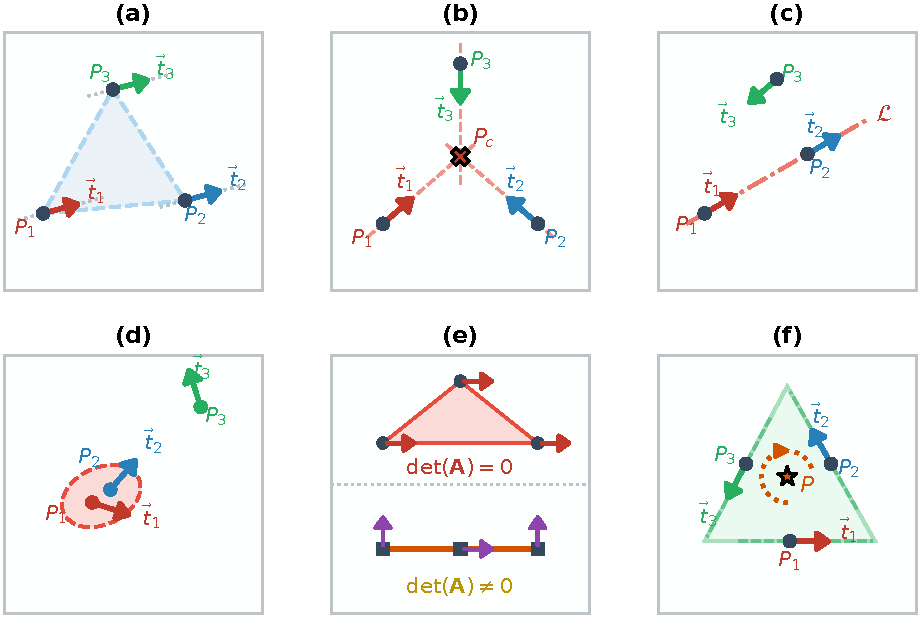
\includegraphics[width=\textwidth]{figura_singularidades_matriz_A.pdf}
    \caption{Singularity configurations and support qualification for the VNMM $\mathcal{L}^1$ placement matrix $\mathbf{A}$.
        (a) Global vector parallelism ($\vec{t}_1 \parallel \vec{t}_2 \parallel \vec{t}_3$);
        (b) Concurrent lines of action intersecting at focal point $P_c$;
        (c) Collinear nodes sharing a common line of action;
        (d) Nodal coincidence ($\|P_1 - P_2\| \to 0$);
        (e) Decoupling of nodal geometry and director alignment: spatially non-collinear nodes with parallel directors yield $\det(\mathbf{A}) = 0$ (top), whereas collinear nodes with non-parallel directors fail to span 2D derivatives (bottom);
        (f) Admissible support: non-collinear distribution ($\operatorname{Area}(T) > 0$) with non-vanishing circulation around evaluation point $P$.}
    \label{fig:vnmm_singularities_matrix_A}
\end{figure*}

\begin{enumerate}
    \item \textbf{Global Director Parallelism (Fig.~\ref{fig:vnmm_singularities_matrix_A}a):} If directors are mutually parallel ($\vec{t}_1 \parallel \vec{t}_2 \parallel \vec{t}_3$), $\operatorname{Col}_1(\mathbf{A}) \propto \operatorname{Col}_2(\mathbf{A})$, yielding $\det(\mathbf{A}) \equiv 0$ irrespective of node positions.
    \item \textbf{Concurrent Lines of Action (Fig.~\ref{fig:vnmm_singularities_matrix_A}b):} If director lines of action intersect at a common point $P_c(x_c, y_c)$, $\operatorname{Col}_3 = y_c \operatorname{Col}_1 - x_c \operatorname{Col}_2$, forcing $\det(\mathbf{A}) = 0$.
    \item \textbf{Overlapping Lines of Action (Fig.~\ref{fig:vnmm_singularities_matrix_A}c):} Collinear nodes sharing a common director orientation produce proportional matrix rows ($\operatorname{rank}(\mathbf{A}) \le 2$).
    \item \textbf{Nodal Coincidence (Fig.~\ref{fig:vnmm_singularities_matrix_A}d):} Co-located nodes ($\|\mathbf{x}_i - \mathbf{x}_j\| \to 0$) collapse the spatial moment span.
\end{enumerate}

As illustrated in Fig.~\ref{fig:vnmm_singularities_matrix_A}e, spatial sampling quality is formally decoupled from vector algebraic independence: nodes forming an ideal spatial triangle are singular if directors are parallel ($\det(\mathbf{A})=0$, top), whereas collinear nodes can yield $\det(\mathbf{A})\neq 0$ if directors are non-parallel but fail to span 2D derivatives (bottom). Consequently, an admissible support triad requires dual qualification (Fig.~\ref{fig:vnmm_singularities_matrix_A}f): non-collinear nodal geometry ($|T| > 0$) combined with coherent angular circulation around $P$.

% ---------------------------------------------------------
% SUBSECTION 3.2: SINGULARITY ANALYSIS IN THE COMPLETE P1 BASIS (6x6 MATRIX)
% ---------------------------------------------------------
\subsection{Singularity Characterization via the Null-Space Orthogonality Principle}
\label{subsec:singularities_P1}

Extending the singularity analysis to the complete vector basis $\mathcal{P}^1$ ($M_{\mathrm{supp}} = 6$), we consider the corresponding $6 \times 6$ local placement matrix $\mathbf{A} \in \mathbb{R}^{6 \times 6}$ defined in Eq.~\eqref{eq:matrix_A_6x6}. In local translated coordinates centered at the evaluation point $P(x_P, y_P)$ ($\Delta x_k = x_k - x_P, \Delta y_k = y_k - y_P$), any coefficient vector $\mathbf{p} = [a_1, a_2, b_1, b_2, b_3, b_4]^T \in \mathbb{R}^6$ uniquely defines an affine vector field $\vec{E}(\mathbf{x}) \in \mathcal{P}^1$:
\begin{equation}
    \vec{E}(\mathbf{x}) = \begin{bmatrix} a_1 + b_1 \Delta x + b_2 \Delta y \\[2pt] a_2 + b_3 \Delta x + b_4 \Delta y \end{bmatrix}.
\end{equation}
By construction, the $k$-th row of the homogeneous placement system $\mathbf{A}\mathbf{p} = \mathbf{0}$ computes the pointwise directional projection $\vec{E}(\mathbf{x}_k) \cdot \vec{t}_k = 0$. This establishes the \textbf{Null-Space Orthogonality Principle}:
\begin{equation}
    \mathbf{p} \in \ker(\mathbf{A}) \iff \vec{E}(\mathbf{x}_k) \cdot \vec{t}_k = 0, \quad \forall k \in \{1, \dots, 6\}.
    \label{eq:null_space_orthogonality}
\end{equation}
Consequently, exact algebraic singularity ($\det(\mathbf{A}) = 0$) occurs if and only if there exists a non-trivial affine vector field $\vec{E} \in \mathcal{P}^1 \setminus \{\mathbf{0}\}$ that is pointwise orthogonal to all six nodal directors at their respective spatial positions.

In the 24-dimensional configuration space of support node coordinates and director orientations $\{(\mathbf{x}_k, \vec{t}_k)\}_{k=1}^6$, this orthogonality criterion defines a continuous algebraic hypersurface $\det(\mathbf{A}) = 0$. Unlike the 3-node basis $\mathcal{L}^1$ where singular geometries admit straightforward spatial classifications (Fig.~\ref{fig:vnmm_singularities_matrix_A}), the complete 6-node space $\mathcal{P}^1$ couples spatial coordinates and angular orientations into a rich manifold: $\mathbf{A}$ becomes singular whenever directors align with the local normals of an affine vector field, even on non-collinear point distributions with mutually non-parallel directors. Configurations in the immediate neighborhood of this hypersurface produce severely ill-conditioned matrices. Attempting to enumerate isolated geometric pathologies via heuristic decision trees is therefore intrinsically incomplete, establishing the necessity of qualifying candidate sextets directly through a unified algebraic metric.


% ---------------------------------------------------------
% SECTION 3.3: AUTOMATED SUPPORT SELECTION ALGORITHM
% ---------------------------------------------------------
\subsection{Automated Support Selection Algorithm via Scale-Invariant Dimensionless Matrix}
\label{sec:support_selection_algorithm}

As established in Section~\ref{subsec:singularities_P1}, matrix singularity in the VNMM local placement system ($\mathbf{A} \boldsymbol{\beta}_i = \mathbf{L}_i$) is governed by the Null-Space Orthogonality Principle, forming an algebraic hypersurface in configuration space. Because singular and near-singular configurations arise whenever nodal directors approach pointwise orthogonality to an affine field in $\mathcal{P}^1$---regardless of whether the point distribution appears geometrically well-spread---heuristic geometric selection schemes relying on conditional decision trees are incomplete and unreliable.

In contrast, evaluating the magnitude of the determinant $|\det(\mathbf{A}_{6\times6})|$ of the local placement matrix serves as a unified algebraic filter against exact and near-singular configurations. Because $\mathbf{A}_{6\times6}$ incorporates both spatial coordinates and vector director projections within a single operator, enforcing $|\det(\mathbf{A}_{6\times6})| \ge \mathrm{Tol}$ simultaneously screens out all configurations on the null-space orthogonality hypersurface as well as candidate sextets in their ill-conditioned near-singular vicinity.

% ---------------------------------------------------------
% SUBSECTION 3.3.1: SCALE-INVARIANT DIMENSIONLESS MATRIX
% ---------------------------------------------------------
\subsubsection{Scale-Invariant Support Selection via Dimensionless Matrix}
\label{subsec:scale_invariant_criterion}

In local translated coordinates centered at the evaluation point $P(x_P, y_P)$, the first two columns of the classical placement matrix $\mathbf{A} \in \mathbb{R}^{6 \times 6}$ consist of dimensionless unit director components $t_{kx}, t_{ky} \sim \mathcal{O}(1)$, while columns 3--6 contain products of coordinates and directors, $\Delta x_k t_{kx}, \Delta y_k t_{kx}, \Delta x_k t_{ky}, \Delta y_k t_{ky} \sim \mathcal{O}(h)$ [m], where $h$ denotes the local characteristic nodal spacing. Consequently, the standard placement matrix has mixed physical units ($[L]^0$ and $[L]^1$), and its determinant scales quartically:
\begin{equation}
    \det(\mathbf{A}_{6\times6}) \sim \mathcal{O}(h^4).
    \label{eq:det_quartic_scaling}
\end{equation}
Directly qualifying candidate stencils using the dimensional determinant introduces two severe difficulties:
\begin{enumerate}
    \item \textbf{Scale Coupling and Threshold Decay:} Because $\det(\mathbf{A}) \propto h^4$, the determinant decays rapidly under spatial refinement ($h \to 0$), preventing the definition of a universal, scale-independent threshold across arbitrary domain sizes or multiscale meshes.
    \item \textbf{Condition Number Inflation:} The mixed physical units create an artificial scaling imbalance between columns 1--2 ($\mathcal{O}(1)$) and columns 3--6 ($\mathcal{O}(h)$), inflating the 2-norm condition number as $\kappa_2(\mathbf{A}) \propto \mathcal{O}(1/h)$ as $h \to 0$ purely as a metric artifact.
\end{enumerate}

To eliminate this $\mathcal{O}(h^4)$ scaling dependence and decouple algebraic qualification from physical dimensions, local spatial coordinates are normalized by a characteristic local length scale $h_{\mathrm{local}} > 0$. For general point distributions, $h_{\mathrm{local}}$ is defined deterministically as the mean Euclidean distance to the first six nearest spatial neighbors retrieved from the $k$-d tree:
\begin{equation}
    h_{\mathrm{local}}(\mathbf{x}_P) = \frac{1}{6} \sum_{k=1}^6 \|\mathbf{x}_{(k)} - \mathbf{x}_P\|,
    \label{eq:h_local_canonical}
\end{equation}
or uniformly as $h_{\mathrm{local}} = h_{\mathrm{nom}}$ on quasi-uniform point clouds with nominal spacing $h_{\mathrm{nom}}$ (Section~\ref{sec:numerical_results}).
Using normalized dimensionless local coordinates $\hat{x}_k = \Delta x_k / h_{\mathrm{local}}$ and $\hat{y}_k = \Delta y_k / h_{\mathrm{local}}$, row $k$ of the dimensionless matrix $\widehat{\mathbf{A}} \in \mathbb{R}^{6 \times 6}$ is assembled as:
\begin{equation}
    \widehat{\mathbf{A}}_{k, :} = \begin{bmatrix} t_{kx} & t_{ky} & \hat{x}_k t_{kx} & \hat{y}_k t_{kx} & \hat{x}_k t_{ky} & \hat{y}_k t_{ky} \end{bmatrix}, \quad k = 1, \dots, 6.
    \label{eq:matrix_A_hat_definition}
\end{equation}
The dimensional matrix $\mathbf{A}$ and its dimensionless counterpart $\widehat{\mathbf{A}}$ satisfy the exact diagonal relation:
\begin{equation}
    \mathbf{A} = \widehat{\mathbf{A}} \, \mathbf{D}_h, \quad \text{with } \mathbf{D}_h = \operatorname{diag}(1, \; 1, \; h_{\mathrm{local}}, \; h_{\mathrm{local}}, \; h_{\mathrm{local}}, \; h_{\mathrm{local}}),
    \label{eq:matrix_factorization_Dh}
\end{equation}
which establishes the determinant identity:
\begin{equation}
    \det(\mathbf{A}) = h_{\mathrm{local}}^4 \det(\widehat{\mathbf{A}}) \implies |\det(\widehat{\mathbf{A}})| = \frac{|\det(\mathbf{A})|}{h_{\mathrm{local}}^4}.
    \label{eq:dimensionless_det_relation}
\end{equation}
Support qualification is thus formulated directly on the dimensionless determinant:
\begin{equation}
    |\det(\widehat{\mathbf{A}})| \ge \widehat{\mathrm{Tol}} > 0,
    \label{eq:dimensionless_threshold_criterion}
\end{equation}
where $\widehat{\mathrm{Tol}} \sim \mathcal{O}(1)$ is a universal threshold (e.g., $\widehat{\mathrm{Tol}} \in [0.05, 1.50]$). Operating on $\widehat{\mathbf{A}}$ simultaneously resolves threshold decay and clears the artificial $\mathcal{O}(1/h)$ penalty from $\kappa_2(\widehat{\mathbf{A}})$, preserving compact nearest-neighbor stencils ($K_{\mathrm{avg}} \approx 6.5\text{--}7.1$ on Cartesian lattices, Table~\ref{tab:support_selection_cost}, and $7.7\text{--}8.2$ on irregular clouds, Section~\ref{subsec:spectral_irregular_clouds}) without support dilation as $h \to 0$.

Any alternate length scale $h_{\mathrm{local}} \to c \, h_{\mathrm{local}}$ transforms the determinant quartically:
\begin{equation}
    |\det(\widehat{\mathbf{A}})| \longrightarrow c^{-4} |\det(\widehat{\mathbf{A}})|.
    \label{eq:quartic_h_local_scaling}
\end{equation}
Because candidate stencils are bounded within the immediate neighborhood ($\|\hat{\mathbf{x}}_k\| \le C$), the spectral norm is bounded by the Frobenius norm ($\sigma_{\max}^2 \le \|\widehat{\mathbf{A}}\|_F^2 \le 6(1+C^2)$) \cite{golub2013matrix}. Since $|\det(\widehat{\mathbf{A}})| \le \sigma_{\min}\sigma_{\max}^5$, enforcing $|\det(\widehat{\mathbf{A}})| \ge \widehat{\mathrm{Tol}}$ guarantees $\sigma_{\min} \ge \widehat{\mathrm{Tol}}/\sigma_{\max}^5 > 0$, effectively controlling conditioning ($\kappa_2(\widehat{\mathbf{A}}) \le 5.9$ under $25\%$ jitter; Section~\ref{subsec:stochastic_perturbations}).

The vector shape functions and spatial derivatives at $P$ are obtained directly from $\widehat{\boldsymbol{\beta}} = \widehat{\mathbf{A}}^{-1}$ via $\boldsymbol{\beta} = \mathbf{D}_h^{-1} \widehat{\boldsymbol{\beta}}$:
\begin{align}
    \vec{N}_i(P)                & = \begin{bmatrix} \hat{\beta}_{1i} \\ \hat{\beta}_{2i} \end{bmatrix}, \label{eq:shape_func_hat_eval}        \\
    (\nabla \times \vec{N}_i)_z & = \frac{1}{h_{\mathrm{local}}} \left( \hat{\beta}_{5i} - \hat{\beta}_{4i} \right), \label{eq:curl_hat_eval} \\
    \nabla \cdot \vec{N}_i      & = \frac{1}{h_{\mathrm{local}}} \left( \hat{\beta}_{3i} + \hat{\beta}_{6i} \right), \label{eq:div_hat_eval}
\end{align}
factoring out the $\mathcal{O}(h^{-1})$ gradient scaling analytically through $1/h_{\mathrm{local}}$.

\subsubsection{The 4-Phase Selection Pipeline}
\label{subsec:4phase_pipeline}

To locate well-conditioned candidate sextets across unstructured point clouds without exhaustive $\mathcal{O}(N^2)$ evaluations, the selection framework couples orthogonal $k$-d tree spatial queries \cite{bentley1975multidimensional,parreira2006efficient,fasshauer2007meshfree,goncalves2025tese,wu2026high} with dimensionless algebraic qualification in a 4-phase pipeline:
\begin{enumerate}
    \item \textbf{Phase 1: Spatial Neighborhood Query via $k$-d Tree:} An orthogonal $k$-d tree ($\mathcal{O}(N \log N)$ one-off construction) queries the $K_{\mathrm{initial}} \ge 12$ nearest neighbors of $P(x_P, y_P)$ with average complexity $\mathcal{O}(\log N)$, defining $h_{\mathrm{local}}$ via Eq.~\eqref{eq:h_local_canonical}.
    \item \textbf{Phase 2: Proximity-Ordered Candidate Generation:} Candidate sextets are generated by fixing the node closest to $P$ as an anchor and taking 5-combinations from subsequent nearest neighbors, ordered by increasing mean distance.
    \item \textbf{Phase 3: Dimensionless Matrix Assembly:} Local coordinates are normalized ($\hat{x}_k = \Delta x_k/h_{\mathrm{local}}, \hat{y}_k = \Delta y_k/h_{\mathrm{local}}$) and $\widehat{\mathbf{A}}_{6 \times 6}$ is assembled via Eq.~\eqref{eq:matrix_A_hat_definition}.
    \item \textbf{Phase 4: Dimensionless Qualification with Early Stopping:} The first candidate sextet satisfying $|\det(\widehat{\mathbf{A}}_{6\times6})| \ge \widehat{\mathrm{Tol}}$ (Eq.~\eqref{eq:dimensionless_threshold_criterion}) is immediately accepted, terminating the search loop.
\end{enumerate}

\subsubsection{Computational Complexity and Combinatorial Cost Analysis}
\label{subsubsec:computational_complexity}

While an initial neighborhood of $K_{\mathrm{initial}} = 12$ nodes yields a theoretical worst-case bound of:
\begin{equation}
    N_{\mathrm{comb}}^{\mathrm{max}} = \binom{K_{\mathrm{initial}}}{6} = \binom{12}{6} = 924 \text{ combinations},
    \label{eq:binomial_combinations}
\end{equation}
early stopping terminates the search as soon as an admissible support is found. As a result, the actual qualification count $\bar{N}_{\mathrm{tested}}$ evaluates only a minimal fraction of these combinations. The total operational runtime across $N_{\mathrm{eval}}$ evaluation points is:
\begin{align}
    T_{\mathrm{support}} & = \underbrace{\mathcal{O}(N \log N)}_{\text{$k$-d tree construction}}
    + \sum_{p=1}^{N_{\mathrm{eval}}} \left[ \underbrace{\mathcal{O}(\log N)}_{\text{spatial query}} + \underbrace{\bar{N}_{\mathrm{tested}}^{(p)} \, C_{\det(6 \times 6)}}_{\text{observed algebraic qualification}} \right].
    \label{eq:support_total_complexity}
\end{align}

Table~\ref{tab:support_selection_cost} reports the empirical performance metrics measured across the six cavity refinement levels of Section~\ref{subsec:convergence_comparison} ($3 \times 3$ Gauss quadrature, $N_g$ scaling from $1{,}764$ to $20{,}736$, $\widehat{\mathrm{Tol}} = 0.80$). Across all levels, the mean qualification count $\bar{N}_{\mathrm{tested}}$ ranges from only $4.73$ to $5.95$ sextets (with maximum evaluations never exceeding $87$). Support selection consumes merely $42\text{--}51\,\mu\text{s}$ per Gauss point ($t_{\mathrm{sup}} = 0.091\text{--}0.881$\,s, representing $44\%\text{--}49\%$ of total assembly time $t_{\mathrm{ass}}$). Even under $25\%$ spatial jitter and random directors (Section~\ref{subsec:stochastic_perturbations}), early stopping tests an average of $\bar{N}_{\mathrm{tested}} \approx 48\text{--}120$ candidates ($< 1$\,ms per evaluation point). Consequently, support selection is dominated by the logarithmic spatial neighbor query rather than combinatorial matrix evaluations.

\begin{table}[!htbp]
    \centering
    \caption{Computational cost of automated support selection across the six cavity discretization levels of Section~\ref{subsec:convergence_comparison} ($3 \times 3$ Gauss-Legendre quadrature, $\widehat{\mathrm{Tol}} = 0.80$, $K_{\mathrm{initial}} = 12$).}
    \label{tab:support_selection_cost}
    \resizebox{\columnwidth}{!}{%
        \begin{tabular}{@{} c c c c c c c c @{}}
            \toprule
            \textbf{Grid Mesh} & \textbf{DoFs}      & \textbf{Gauss Points} & \textbf{Mean Neighbors} & \multicolumn{2}{c}{\textbf{Evaluated Sextets ($N_{\mathrm{tested}}$)}} & \textbf{Support Time} & \textbf{Assembly Time}                          \\
            \cmidrule(lr){5-6}
            $N_v \times N_v$   & $N_{\mathrm{DoF}}$ & $N_g$                 & $K_{\mathrm{avg}}$      & \textbf{Mean} ($\bar{N}_{\mathrm{tested}}$)                            & \textbf{Maximum}      & $t_{\mathrm{sup}}$ [s] & $t_{\mathrm{ass}}$ [s] \\
            \midrule
            $15 \times 15$     & 169                & $1{,}764$             & 6.56                    & $\mathbf{5.95}$                                                        & 87                    & 0.091                  & 0.187                  \\
            $22 \times 22$     & 400                & $3{,}969$             & 6.53                    & $\mathbf{5.42}$                                                        & 87                    & 0.186                  & 0.414                  \\
            $29 \times 29$     & 729                & $7{,}056$             & 6.53                    & $\mathbf{5.14}$                                                        & 87                    & 0.321                  & 0.717                  \\
            $36 \times 36$     & 1156               & $11{,}025$            & 6.53                    & $\mathbf{4.96}$                                                        & 87                    & 0.484                  & 1.088                  \\
            $43 \times 43$     & 1681               & $15{,}876$            & 6.49                    & $\mathbf{4.81}$                                                        & 87                    & 0.683                  & 1.529                  \\
            $49 \times 49$     & 2209               & $20{,}736$            & 6.49                    & $\mathbf{4.73}$                                                        & 87                    & 0.881                  & 1.996                  \\
            \bottomrule
        \end{tabular}%
    }
\end{table}


% --- SEÇÃO 4: FORMULAÇÃO DA CAVIDADE ---
% =========================================================
% SECTION 4: VARIATIONAL FORMULATION OF THE RESONANT CAVITY PROBLEM
% =========================================================
\section{Variational Formulation of the Resonant Cavity Problem}
\label{sec:variational_formulation}

To evaluate the spectral accuracy and verify the shifting of non-physical spurious gradient modes outside the operational bandwidth in the Vector Nodal Meshless Method (VNMM 2D), we formulate the electromagnetic vector eigenvalue problem in a two-dimensional resonant cavity $\Omega = [0, \pi] \times [0, \pi] \subset \mathbb{R}^2$ with perfect electric conductor (PEC) walls $\partial\Omega$ \cite{harrington2001time}.

\subsection{The Transverse Electric (\texorpdfstring{$TE_z$}{TEz}) Vector Eigenvalue Problem}
\label{subsec:strong_form}

In a homogeneous, isotropic, and lossless dielectric medium ($\epsilon_r = 1.0, \mu_r = 1.0$), time-harmonic Transverse Electric modes ($TE_z$) are governed by the vector double-curl Helmholtz equation for the transverse electric field $\vec{E}(\mathbf{x}) = [E_x(x,y), E_y(x,y)]^T$ \cite{monk2003finite, ortiz2023tese}:
\begin{align}
    \nabla \times \left( \frac{1}{\mu_r} \nabla \times \vec{E} \right) & = \lambda \, \epsilon_r \vec{E}, \quad \text{in } \Omega \label{eq:helmholtz_strong} \\
    \hat{n} \times \vec{E}                                             & = \mathbf{0}, \quad \text{on } \partial\Omega \label{eq:pec_boundary}
\end{align}
where $\lambda = k_0^2 = \omega^2 \mu_0 \epsilon_0$ denotes the target wavenumber eigenvalue, $\omega$ is the angular resonance frequency, and $\hat{n}$ is the outward unit normal vector to boundary $\partial\Omega$. In two dimensions, the curl operator acting on a 2D vector field yields a scalar normal component $(\nabla \times \vec{E})_z = \partial E_y/\partial x - \partial E_x/\partial y$, while the vector curl of a scalar field $u_z$ returns a vector in the transverse plane $\nabla \times u_z = [\partial u_z/\partial y, -\partial u_z/\partial x]^T$.

The exact analytical eigenvalues for the square PEC cavity are given by \cite{harrington2001time}:
\begin{equation}
    \lambda_{m,n}^{\mathrm{exact}} = m^2 + n^2, \quad m,n \in \{0, 1, 2, \dots\}, \quad (m+n > 0)
    \label{eq:analytical_eigenvalues}
\end{equation}

% ---------------------------------------------------------
% SUBSECTION 4.2: RITZ-GALERKIN WEAK FORM WITH DIV-CURL REGULARIZATION
% ---------------------------------------------------------
\subsection{Ritz-Galerkin Weak Form with Div-Curl Regularization}
\label{subsec:weak_form_regularization}

To solve the vector boundary-value problem~\eqref{eq:helmholtz_strong}--\eqref{eq:pec_boundary} numerically, the strong-form double-curl Helmholtz equation must be recast into a variational weak formulation. In standard electromagnetic field theory, testing the Helmholtz equation against an admissible vector field $\vec{W}$ and applying vector Green's first identity yields the canonical curl-curl weak form. Let the underlying Hilbert space of square-integrable vector fields with square-integrable curl satisfying homogeneous tangential PEC boundary conditions be defined as \cite{monk2003finite, bossavit1998computational, boffi2013mixed}:
\begin{equation}
    \mathcal{S} \triangleq \left\{ \vec{E} \in H(\mathbf{curl}; \Omega) \;\middle|\; \hat{n} \times \vec{E} = \mathbf{0} \text{ on } \partial\Omega \right\}.
    \label{eq:hilbert_space_S}
\end{equation}
The classical, unregularized variational problem seeks eigenpairs $(\lambda, \vec{E}) \in \mathbb{R} \times \mathcal{S} \setminus \{\mathbf{0}\}$ satisfying:
\begin{equation}
    \int_{\Omega} \frac{1}{\mu_r} (\nabla \times \vec{W})_z (\nabla \times \vec{E})_z \, d\Omega = \lambda \int_{\Omega} \epsilon_r \vec{W} \cdot \vec{E} \, d\Omega, \quad \forall \vec{W} \in \mathcal{S}.
    \label{eq:unregularized_weak_form}
\end{equation}
While Eq.~\eqref{eq:unregularized_weak_form} is spectrally well-behaved when discretized using globally conforming N\'ed\'elec edge elements (where exact de Rham sequence preservation confines the infinite-dimensional static gradient nullspace to $\lambda = 0$), implementing this standard formulation directly within a meshless framework triggers severe spectral contamination: non-physical, highly oscillatory spurious modes infiltrate the low-frequency physical spectrum.


\subsubsection{Non-Conforming Variational Structure and Gradient Leakage}
\label{subsubsec:theoretical_origin_leakage}
In standard Edge Finite Element Formulations (EFEM), the discrete space is globally $H(\mathbf{curl})$-conforming ($V_h \subset \mathcal{S}$) because shared tangential degrees of freedom across conforming element facets guarantee exact tangential trace continuity ($\hat{n} \times [\vec{E}^h] = \mathbf{0}$) \cite{monk2003finite, bossavit1998computational}. Under this global conformity, the discrete de Rham complex property $\operatorname{Im}(\nabla) \subset \ker(\nabla \times)$ holds exactly: irrotational gradient fields ($\vec{E} = \nabla \phi$) yield an identically zero curl ($\nabla \times (\nabla \phi) \equiv \mathbf{0}$) and map directly into the zero eigenvalue subspace ($\lambda = 0$), preventing spectrum contamination without auxiliary constraints \cite{monk2003finite, boffi1999computational, boffi2013mixed}.

In contrast, on unconstrained point clouds, the assembled meshless VNMM vector approximation is globally non-conforming:
\begin{equation}
    V_h \not\subset \mathcal{S} \subset H(\mathbf{curl}; \Omega).
    \label{eq:nonconforming_space}
\end{equation}
Although each local shape function $\vec{N}_i(\mathbf{x})$ possesses local $H(\mathbf{curl})$ regularity within its local support stencil (Section~\ref{subsec:complete_P1_basis}), active support stencils are determined dynamically across the domain via $k$-d tree spatial queries. Consequently, discrete fields exhibit small tangential trace discontinuities across the internal boundaries where support configurations change.

In the present formulation, the curl and divergence of the discrete field are evaluated using the classical derivatives of the local VNMM interpolants directly at the background integration points. Bilinear forms are then assembled from these pointwise differential quantities over the background cells. In the absence of explicit interface jump terms or Lagrange multipliers across stencil transitions, this procedure constitutes an elementwise (pointwise) evaluation of the differential operators, rather than an evaluation of the full distributional derivatives associated with a globally conforming $H(\mathbf{curl})$ space.

Accordingly, the discrete scheme represents a non-conforming variational approximation of the continuous Maxwell problem. Its numerical consistency, spectral correctness, and stability cannot be inferred solely from continuous variational theorems or local polynomial completeness; they must be assessed in conjunction with support transitions, boundary constraint enforcement, numerical quadrature, and volumetric regularization. Within the electromagnetic eigenvalue problem, this global non-conformity triggers two interrelated spectral mechanisms:
\begin{enumerate}
    \item \textbf{Non-Inheritance of Discrete de Rham Exactness:} Because tangential traces suffer inter-stencil jumps across shifting support boundaries, the discrete approximation does not inherit the exactness of the continuous de Rham complex. Specifically, discrete gradient fields fail to maintain an identically vanishing numerical curl at integration points:
          \begin{equation}
              \nabla_h \times \nabla_h \phi_h \neq \mathbf{0}.
              \label{eq:grad_curl_nonvanishing}
          \end{equation}
    \item \textbf{Discrete Gradient Nullspace Leakage:} Because $\nabla_h \times \nabla_h \phi_h \neq \mathbf{0}$ at background quadrature points, non-zero numerical curl residues leak the infinite-dimensional static gradient nullspace into the non-zero discrete spectrum, causing non-physical, highly oscillatory spurious modes to corrupt the physical resonance band.
\end{enumerate}

\paragraph{The Methodological Chain}
To counteract these non-conforming mechanisms while preserving the flexibility of a point cloud without topological meshes, the proposed framework establishes a cohesive architectural chain:
\begin{equation}
    \boxed{
        \begin{aligned}
            \mathcal{L}^1 \text{ (derivative defect)}        & \longrightarrow \mathcal{P}^1 \text{ (local completeness)}                \\
                                                             & \;\Downarrow                                                              \\
            \text{dynamic supports}                          & \longrightarrow V_h \not\subset H(\mathbf{curl}) \text{ (non-conformity)} \\
                                                             & \;\Downarrow                                                              \\
            \text{loss of de Rham exactness}                 & \longrightarrow \text{gradient leakage (spurious modes)}                  \\
                                                             & \;\Downarrow                                                              \\
            \mathbf{K}_{\mathrm{div}} \text{ regularization} & \longrightarrow \text{spectral shifting of spurious modes}
        \end{aligned}
    }
    \label{eq:conceptual_chain}
\end{equation}
This causal progression demonstrates that while local polynomial completeness ($\mathcal{P}^1$) is indispensable to resolve the local Jacobian and eliminate derivative aliasing, clearing the operational spectrum from non-conforming gradient leakage on unconstrained point clouds requires shifting spurious modes through the divergence penalty operator developed next.

\subsubsection{Div-Curl Regularized Weak Formulation}
\label{subsubsec:div_curl_weak_form}
To shift these spurious gradient modes outside the operational bandwidth without introducing saddle-point system indefiniteness or auxiliary Lagrange multipliers, we adopt a \textbf{Ritz-Galerkin weak formulation with div-curl penalty regularization} \cite{monk2003finite, bossavit1998computational, boffi2013mixed}:
\begin{multline}
    \int_{\Omega} \frac{1}{\mu_r} (\nabla \times \vec{W})_z (\nabla \times \vec{E})_z \, d\Omega + s_{\mathrm{div}} \int_{\Omega} (\nabla \cdot \vec{W}) (\nabla \cdot \vec{E}) \, d\Omega \\
    = \lambda \int_{\Omega} \epsilon_r \vec{W} \cdot \vec{E} \, d\Omega, \quad \forall \vec{W} \in \mathcal{S}
    \label{eq:regularized_weak_form}
\end{multline}
where $s_{\mathrm{div}} > 0$ is the non-dimensional divergence penalty parameter \cite{monk2003finite}.

Upon discretizing the electric field as $\vec{E}^h(\mathbf{x}) = \sum_{j=1}^{M} e_j \vec{N}_j(\mathbf{x})$ using the scalar projection DoFs $e_j = \vec{E}(\mathbf{x}_j) \cdot \vec{t}_j$ (Eq.~\eqref{eq:dof_projection_definition}) and test functions as $\vec{W}^h(\mathbf{x}) = \sum_{i=1}^{M} d_i \vec{N}_i(\mathbf{x})$ with test coefficients $d_i = \vec{W}(\mathbf{x}_i) \cdot \vec{t}_i$, the second bilinear term in Eq.~\eqref{eq:regularized_weak_form} defines the \textbf{divergence penalty matrix} $\mathbf{K}_{\mathrm{div}} \in \mathbb{R}^{M \times M}$, whose entries $K_{\mathrm{div}, ij}$ are explicitly defined by:
\begin{equation}
    K_{\mathrm{div}, ij} \triangleq \int_{\Omega} (\nabla \cdot \vec{N}_i) (\nabla \cdot \vec{N}_j) \, d\Omega
    \label{eq:K_div_definition}
\end{equation}

Consequently, the global stiffness matrix $\mathbf{K}$ in the discrete generalized eigenvalue problem $\mathbf{K} \mathbf{e} = \lambda \mathbf{M} \mathbf{e}$ decomposes into the sum of the primary curl-curl stiffness matrix $\mathbf{K}_{\mathrm{curl}}$ and the scaled divergence penalty matrix $s_{\mathrm{div}} \mathbf{K}_{\mathrm{div}}$:
\begin{equation}
    \mathbf{K} = \mathbf{K}_{\mathrm{curl}} + s_{\mathrm{div}} \mathbf{K}_{\mathrm{div}}
    \label{eq:K_global_decomposition}
\end{equation}
with individual entries of the primary curl-curl stiffness matrix defined by:
\begin{equation}
    K_{\mathrm{curl}, ij} \triangleq \int_{\Omega} \frac{1}{\mu_r} (\nabla \times \vec{N}_i)_z (\nabla \times \vec{N}_j)_z \, d\Omega.
    \label{eq:K_curl_definition}
\end{equation}

\paragraph{Consistency, Stability, and Scope of the Discrete Scheme}
To clearly distinguish the mathematical properties of the discrete scheme, three conceptual levels must be differentiated:
\begin{enumerate}
    \item \textbf{Local Polynomial Consistency:} The complete $\mathcal{P}^1$ basis provides local polynomial completeness and enables the exact reproduction of affine vector fields within the corresponding interpolation stencils. This property supports the consistency of the local field approximation and its first-order spatial derivatives.
    \item \textbf{Algebraic Spectral Regularization:} The div-curl penalty adds a symmetric positive-semidefinite contribution $s_{\mathrm{div}} \mathbf{K}_{\mathrm{div}}$ associated with the discrete divergence, designed to penalize irrotational gradient states that exhibit non-vanishing numerical curl residues due to discrete non-conformity.
    \item \textbf{Non-Conforming Boundaries and Scope:} These properties do not establish global $H(\mathbf{curl})$ conformity or, by themselves, a uniform stability estimate for the assembled non-conforming method; a dedicated analysis of tangential jumps and stability limitations is formalized in Section~\ref{subsubsec:tangential_jump_limitations}.
\end{enumerate}

\paragraph{Operational Mechanisms of Divergence Penalization}
With these theoretical boundaries established, the operational interaction between divergence penalization, nullspace control, and physical field fidelity is structured into four complementary mechanisms \cite{monk2003finite, bossavit1998computational, boffi2013mixed}:
\begin{enumerate}
    \item \textbf{Volumetric Regularization and Domain Topology:} The penalty term $s_{\mathrm{div}} \int_\Omega (\nabla \cdot \vec{W})(\nabla \cdot \vec{E}) \, d\Omega$ provides elliptic regularization in $H(\mathbf{curl}) \cap H(\mathrm{div})$ \cite{monk2003finite, boffi2013mixed}. In simply connected domains with homogeneous PEC walls, the static curl nullspace $\ker(\nabla \times) = \nabla H_0^1(\Omega)$ contains no non-trivial harmonic fields ($\Delta \phi = 0 \implies \phi \equiv 0$), ensuring that all static gradient fields have non-zero divergence ($\Delta \phi \neq 0$) and are penalizable (multiply connected domains or re-entrant corners would require cuts or weighted regularization \cite{bossavit1998computational, gross2004electromagnetic, costabel1991coercive, costabel2002weighted}).
    \item \textbf{Selective Spectral Shifting via Divergence Energy:} Upon activating $s_{\mathrm{div}} \mathbf{K}_{\mathrm{div}}$, the discrete Rayleigh quotient expands as:
          \begin{equation}
              \lambda(\mathbf{e}) = \frac{\mathbf{e}^T \mathbf{K}_{\mathrm{curl}} \mathbf{e}}{\mathbf{e}^T \mathbf{M} \mathbf{e}} + s_{\mathrm{div}} \frac{\mathbf{e}^T \mathbf{K}_{\mathrm{div}} \mathbf{e}}{\mathbf{e}^T \mathbf{M} \mathbf{e}}.
              \label{eq:rayleigh_penalty_expansion}
          \end{equation}
          Because non-physical gradient states have $\nabla \cdot (\nabla \phi) = \Delta \phi \neq 0$, their divergence energy shifts their eigenvalues upward proportional to $s_{\mathrm{div}}$, clearing the low-frequency operational bandwidth (Sections~\ref{subsubsec:modewise_validation} and~\ref{subsubsec:s_div_sensitivity}).
    \item \textbf{Metric for Solenoidal Field Integrity and Mode Classification ($R_{\mathrm{div}}$):} We define the discrete divergence-to-curl energy quotient:
          \begin{equation}
              R_{\mathrm{div}}(\mathbf{e}) \triangleq \frac{\mathbf{e}^T \mathbf{K}_{\mathrm{div}} \mathbf{e}}{\mathbf{e}^T \mathbf{K}_{\mathrm{curl}} \mathbf{e}}.
              \label{eq:R_div_ratio_def}
          \end{equation}
          This metric establishes an explicit quantitative criterion for spectral mode classification:
          \begin{itemize}
              \item \textbf{Physical Modes:} True electromagnetic resonances correspond to solenoidal states ($\nabla \cdot \vec{E} = 0, \nabla \times \vec{E} \neq \mathbf{0}$) converging to analytical Maxwell cavity modes, characterized by $R_{\mathrm{div}}(\mathbf{e}) \ll 1$ (empirically $R_{\mathrm{div}} \le 1.65\%$ in our simulations).
              \item \textbf{Spurious (Gradient) Modes:} Non-physical states originating from discrete gradient nullspace leakage ($\nabla_h \times \nabla_h \phi_h \neq \mathbf{0}$) are irrotational fields with high volumetric divergence ($\Delta \phi \neq 0$), yielding $R_{\mathrm{div}}(\mathbf{e}) \gg 1$ (typically $R_{\mathrm{div}} \sim 10^3\%\text{--}10^6\%$). In this formulation, every observed spurious mode is an irrotational gradient state.
          \end{itemize}
          Throughout this work, the \textbf{operational bandwidth} (or operational spectrum) is defined as the low-frequency interval of physical interest $\Lambda_{\mathrm{op}} \triangleq (0, \lambda_{\max}^{\mathrm{op}}]$ (set to $\lambda_{\max}^{\mathrm{op}} = 10.0$ to encompass the first ten physical cavity modes). The operational spectrum is considered fully purified when all spurious gradient modes satisfy $\lambda_{\mathrm{spur}} > \lambda_{\max}^{\mathrm{op}}$.
    \item \textbf{Spectral Shifting vs. Volumetric Locking:} At the continuous level, solenoidal modes satisfy $\nabla \cdot \vec{E} \equiv 0$, so the penalty vanishes identically. On discrete meshless stencils, pointwise divergence is satisfied only to discretization order ($\nabla \cdot \vec{E}^h \sim \mathcal{O}(h) \neq 0$). Consequently, excessive penalization introduces volumetric stiffening (locking), slightly perturbing physical eigenvalues and elevating matrix conditioning. A calibrated operating window ($s_{\mathrm{div}} \in [6.0, 10.0]$) achieves spectral clearance without locking (Section~\ref{subsubsec:s_div_sensitivity}).
\end{enumerate}

\subsubsection{Tangential-Jump Control and Limitations of the Present Formulation}
\label{subsubsec:tangential_jump_limitations}

The lack of global tangential continuity is a distinct source of non-conformity that is not directly controlled by the divergence penalty. In particular, a small discrete divergence does not necessarily imply a small tangential jump across a support-transition interface. Therefore, the div-curl regularization should be interpreted as a mechanism for mitigating the observed gradient-related spectral contamination, rather than as a general enforcement of $H(\mathbf{curl})$ conformity.

In the present implementation, no explicit penalty term is introduced for tangential jumps across support-transition interfaces. The influence of these transitions is instead assessed indirectly through the manufactured-solution convergence tests and the spectral experiments reported in Section~\ref{sec:numerical_results}. Accordingly, the numerical results demonstrate the effectiveness of the proposed regularization for the configurations considered, but do not establish a uniform bound on tangential jumps or a general stability guarantee for arbitrary point clouds.

An explicit tangential-jump stabilization (e.g., drawing on Interior Penalty Discontinuous Galerkin techniques \cite{houston2004mixed, hesthaven2004high}), or a rigorous estimate showing that the corresponding non-conformity error remains controlled under refinement, is an important direction for further work.



\subsection{Integration Strategy: Cell-Based vs. Point-Based (EFG-Style)}
\label{subsec:integration_strategy}

Numerical evaluation of weak form integrals in Eq.~\eqref{eq:regularized_weak_form} requires background cell quadrature. In early VNMM implementations, support nodes and placement matrices $\mathbf{A}$ were constructed once per cell at its centroid $P_c$ \cite{ortiz2021nodal, ortiz2023tese}. However, expanding shape functions across large cells ($dx > h$) induces severe Taylor truncation errors.

To obtain a mesh-connectivity-free field approximation, we employ a point-based Element-Free Galerkin (EFG) integration strategy \cite{belytschko1994element, parreira2006efficient}:
\begin{enumerate}
    \item \textbf{Background Integration Scaffolding:} A resolution-matched background Cartesian grid of $N_{cx} \times N_{cy} = (N_v - 1) \times (N_v - 1)$ quadrilateral cells ($dx = dy = h_{\mathrm{nom}}$) covers $\Omega$ with $3 \times 3$ Gauss-Legendre quadrature ($N_g / N_{\mathrm{DoF}} \approx 10$), avoiding under-integration artifacts (Section~\ref{subsubsec:quadrature_sensitivity}).
    \item \textbf{Pointwise Support Selection (Section~\ref{subsec:4phase_pipeline}):} At each Gauss integration point $P_g$, an admissible support sextet $\{P_k, \vec{t}_k\}_{k=1}^6$ is determined on-the-fly via $k$-d tree queries and scale-invariant determinant qualification ($|\det(\widehat{\mathbf{A}}_{6 \times 6})| \ge \widehat{\mathrm{Tol}}$).
    \item \textbf{Pointwise Shape Function Evaluation (Section~\ref{subsec:scale_invariant_criterion}):} Anchoring coordinates directly at $P_g$ ($\Delta x = 0, \Delta y = 0$), vector shape functions $\vec{N}_i(P_g)$ and spatial derivatives $(\nabla \times \vec{N}_i, \nabla \cdot \vec{N}_i)$ are evaluated via Eqs.~\eqref{eq:shape_func_hat_eval}--\eqref{eq:div_hat_eval}, with $1/h_{\mathrm{local}}$ factored out analytically.
\end{enumerate}

Following classical meshfree classification \cite{belytschko1994element, atluri2002meshless, liu2009mesh}, the VNMM field approximation and shape functions are meshless and connectivity-free; background cells serve solely as geometric integration scaffolding without constraining the interpolation topology.

\subsection{Algebraic Discretization and Generalized Eigenvalue System}
\label{subsec:algebraic_system}

Under the discrete field representations $\vec{E}^h$ and $\vec{W}^h$ introduced in Section~\ref{subsubsec:div_curl_weak_form}, substituting the vector shape functions into the regularized weak form~\eqref{eq:regularized_weak_form} yields the global generalized algebraic eigenvalue problem $\mathbf{K} \mathbf{e} = \lambda \mathbf{M} \mathbf{e}$ \cite{ortiz2023tese, goncalves2025tese}. The global regularized stiffness matrix $\mathbf{K} = \mathbf{K}_{\mathrm{curl}} + s_{\mathrm{div}} \mathbf{K}_{\mathrm{div}} \in \mathbb{R}^{M \times M}$ is assembled directly from the curl-curl and divergence penalty blocks defined in Eqs.~\eqref{eq:K_div_definition}--\eqref{eq:K_curl_definition}, whereas the entries of the global mass matrix $\mathbf{M} \in \mathbb{R}^{M \times M}$ are governed by the permittivity-weighted bilinear product on the right-hand side of Eq.~\eqref{eq:regularized_weak_form}:
\begin{equation}
    M_{ij} \triangleq \int_{\Omega} \epsilon_r \, \vec{N}_i \cdot \vec{N}_j \, d\Omega.
    \label{eq:mass_matrix_entry}
\end{equation}

Homogeneous PEC boundary conditions are collocated directly at boundary nodes by setting $e_k = 0$ for all boundary nodes whose unit directors $\vec{t}_k$ align tangent to $\partial\Omega$ ($\vec{t}_k \parallel \partial\Omega$), which enforces $\vec{E}^h(\mathbf{x}_k) \cdot \vec{t}_k = 0$ pointwise \cite{ortiz2021nodal, goncalves2025tese}. Eliminating these constrained degrees of freedom yields the reduced algebraic eigenvalue system:
\begin{equation}
    \mathbf{K}_{\mathrm{red}} \mathbf{e}_{\mathrm{red}} = \lambda \mathbf{M}_{\mathrm{red}} \mathbf{e}_{\mathrm{red}},
    \label{eq:generalized_eigenvalue_system}
\end{equation}
of size $M_{\mathrm{red}} \times M_{\mathrm{red}}$ (equivalently designated as $N_{\mathrm{DoF}} \equiv M_{\mathrm{red}}$ in subsequent convergence comparisons).

While the unregularized Maxwell stiffness operator is symmetric positive-semidefinite due to the static gradient nullspace, the inclusion of the divergence penalty ($s_{\mathrm{div}} > 0$) combined with essential PEC boundary constraints renders $\mathbf{K}_{\mathrm{red}}$ positive-definite on the discrete physical subspace, while the mass matrix $\mathbf{M}_{\mathrm{red}}$ is natively positive-definite. This ensures that the discrete generalized eigenvalue problem involves well-behaved, sparse symmetric positive-definite (SPD) reduced matrices, allowing efficient and stable computation of the physical spectrum using Krylov-subspace shift-and-invert Lanczos methods \cite{saad2011numerical, lehoucq1998arpack}, as implemented via the ARPACK solver (\texttt{eigsh}) in SciPy \cite{virtanen2020scipy}.

% =========================================================
% SECTION 5: NUMERICAL RESULTS AND DISCUSSION
% =========================================================
\section{Numerical Verification and Validation}
\label{sec:numerical_results}

This section assesses the numerical performance of the proposed Vector Nodal Meshless Method over the canonical domain $\Omega = [0, \pi]^2$, organized into three complementary parts: (1)~\textbf{Numerical Verification (Sections~\ref{subsec:conforming_dual_equivalence}--\ref{subsec:patch_test_galerkin}):} local dual equivalence against Whitney elements, restoration of asymptotic curl convergence via $\mathcal{P}^1$, algebraic stencil conditioning under spatial-directional jitter, and linear completeness and asymptotic convergence via the Galerkin Patch Test and MMS; (2)~\textbf{Physics-Based Spectral Validation (Sections~\ref{subsec:cavity_eigenvalues}--\ref{subsec:spectral_irregular_clouds}):} resonant cavity spectra under div-curl penalty regularization, parametric sensitivity of $s_{\mathrm{div}}$, comparative convergence benchmarking against Edge FEM, and spectral validation on irregular point clouds; and (3)~\textbf{Methodological Scope and Boundaries (Section~\ref{subsec:limitations_scope}):} operational boundaries, background quadrature scaffolding, boundary stencil starvation along curved geometries, high-frequency dispersion, and extensions to 3D domains.

\paragraph{Baseline Computational Setup and Operational Conventions}
To ensure methodological consistency and eliminate repetitive descriptions, Table~\ref{tab:baseline_computational_setup} establishes the uniform baseline conventions and parameters adopted throughout Section~\ref{sec:numerical_results}. Because Section~\ref{subsec:conforming_dual_equivalence} evaluates $\mathcal{L}^1$ at triangular midpoints without dynamic selection, $\widehat{\mathbf{A}}$ and $h_{\mathrm{local}}$ are not invoked there.

\begin{table}[!htbp]
    \centering
    \footnotesize
    \renewcommand{\arraystretch}{0.88}
    \setlength{\tabcolsep}{3.5pt}
    \caption{Baseline computational setup, geometric discretizations, and operational solver conventions across Section~\ref{sec:numerical_results}.}
    \label{tab:baseline_computational_setup}
    \begin{tabularx}{\linewidth}{@{}
        >{\raggedright\arraybackslash}p{0.21\linewidth}
        >{\raggedright\arraybackslash}X
        >{\raggedright\arraybackslash}p{0.26\linewidth}
        @{}}
        \toprule
        \textbf{Convention / Parameter}                                                                                                                                                                                                                                                                     &
        \textbf{Mathematical Specification / Operational Formulation}                                                                                                                                                                                                                                       &
        \textbf{Applicable Benchmarks}                                                                                                                                                                                                                                                                        \\
        \midrule
        \textbf{Domain \& Interior Grid}                                                                                                                                                                                                                                                                    &
        $\Omega = [0, \pi]^2$, reference grid with $N_x \times N_y$ nodes ($N_x = N_y$), nominal spacing $h_{\mathrm{nom}} = \pi / (N_x - 1)$. \newline
        Cartesian interior coordinates: $\mathbf{x}_{i,j} = (i\,h_{\mathrm{nom}}, \; j\,h_{\mathrm{nom}})$ for $i, j = 1, \dots, N_x - 2$.                                                                                                                                                                  &
        All benchmarks without exception (Secs.~\ref{subsec:conforming_dual_equivalence}--\ref{subsec:spectral_irregular_clouds})                                                                                                                                                                             \\
        \textbf{Staggered Boundary Nodes}                                                                                                                                                                                                                                                                   &
        Midpoints along $\partial\Omega$ edges ($N_{\mathrm{bnd}} = 4(N_x - 1)$ nodes): \newline
        $y \in \{0, \pi\}: \mathbf{x}_k = ((k + \frac{1}{2})h_{\mathrm{nom}}, y), \, \vec{t}_k = [1, 0]^T$; \quad $x \in \{0, \pi\}: \mathbf{x}_k = (x, (k + \frac{1}{2})h_{\mathrm{nom}}), \, \vec{t}_k = [0, 1]^T$. \newline
        Distance $\ge h_{\mathrm{nom}}/2$ from corners. Homogeneous PEC: $e_k = 0$.                                                                                                                                                                                                                         &
        Cavity Dirichlet and PEC benchmarks (Secs.~\ref{subsec:patch_test_galerkin}--\ref{subsec:spectral_irregular_clouds})                                                                                                                                                                                  \\
        \textbf{Internal Directors (Structured)}                                                                                                                                                                                                                                                            &
        Checkerboard alternating orthogonal unit orientations: \newline
        $\vec{t}_{i,j} = [\frac{\sqrt{2}}{2}, \; \frac{\sqrt{2}}{2}]^T$ if $(i+j)$ is even; \quad
        $\vec{t}_{i,j} = [-\frac{\sqrt{2}}{2}, \; \frac{\sqrt{2}}{2}]^T$ if $(i+j)$ is odd. \newline
        Guarantees local orthogonal diversity ($\vec{t}_{45^\circ} \cdot \vec{t}_{135^\circ} = 0$).                                                                                                                                                                                                         &
        Regular lattice benchmarks (Secs.~\ref{subsec:patch_test_galerkin}--\ref{subsec:convergence_comparison})                                                                                                                                                                                              \\
        \textbf{Stochastic Clouds (Disordered)}                                                                                                                                                                                                                                                             &
        Interior nodes perturbed with $25\%$ spatial jitter and uniform random director orientations: \newline
        $\mathbf{x}_k = \mathbf{x}_k^{(0)} + (\delta x_k, \delta y_k), \quad \delta x_k, \delta y_k \sim \mathcal{U}(-0.25\,h_{\mathrm{nom}}, \; 0.25\,h_{\mathrm{nom}})$ \newline
        $\vec{t}_k = [\cos\theta_k, \; \sin\theta_k]^T, \quad \theta_k \sim \mathcal{U}(0, 2\pi)$. Conforming unit tangents on $\partial\Omega$.                                                                                                                                                            &
        Disordered cloud benchmarks (Secs.~\ref{subsec:arbitrary_meshless_interpolation}, \ref{subsec:stochastic_perturbations}, \ref{subsec:patch_test_galerkin}, \ref{subsec:spectral_irregular_clouds})                                                                                                    \\
        \textbf{Support Qualification \& Scaling}                                                                                                                                                                                                                                                           &
        Scale normalization $h_{\mathrm{local}} = h_{\mathrm{nom}}$ (or metric~\eqref{eq:h_local_canonical}). Qualification threshold $\widehat{\mathrm{Tol}} = 0.80$ with query pool $K_{\mathrm{initial}} = 12$ nearest neighbors ($|\det(\widehat{\mathbf{A}}_{6\times6})| \ge \widehat{\mathrm{Tol}}$). &
        All $\mathcal{P}^1$ benchmarks (Secs.~\ref{subsec:arbitrary_meshless_interpolation}--\ref{subsec:spectral_irregular_clouds}); swept in Sec.~\ref{subsec:stochastic_perturbations}                                                                                                                     \\
        \textbf{Div-Curl Regularization}                                                                                                                                                                                                                                                                    &
        Penalty coefficient $s_{\mathrm{div}} = 6.0$ in regularized weak form~\eqref{eq:regularized_weak_form}, shifting gradient nullspace modes out of the operational cavity spectrum while preserving physical accuracy.                                                                                &
        All variational formulations (Secs.~\ref{subsec:patch_test_galerkin}--\ref{subsec:spectral_irregular_clouds}); swept in Sec.~\ref{subsubsec:s_div_sensitivity}                                                                                                                                        \\
        \textbf{Background Quadrature}                                                                                                                                                                                                                                                                      &
        Topologically independent Cartesian grid of $(N_x - 1) \times (N_y - 1)$ cells ($dx = dy = h_{\mathrm{nom}}$) with $3 \times 3$ Gauss-Legendre quadrature ($9$ points/cell, $N_g / N_{\mathrm{DoF}} \approx 10$).                                                                                   &
        All variational formulations (Secs.~\ref{subsec:patch_test_galerkin}--\ref{subsec:spectral_irregular_clouds}); swept in Sec.~\ref{subsubsec:quadrature_sensitivity}                                                                                                                                   \\
        \bottomrule
    \end{tabularx}
\end{table}


\subsection{Local Constructive Equivalence under Conforming Midpoint/Tangent Placement: VNMM \texorpdfstring{$\mathcal{L}^1$}{L1} vs. Whitney EFEM}
\label{subsec:conforming_dual_equivalence}

To establish a rigorous baseline connecting the proposed vector meshless formulation to established finite element theory, this first experiment numerically validates the Local Constructive Equivalence Theorem (Theorem~\ref{thm:dual_equivalence}) established in Section~\ref{subsubsec:formal_proof_dual_whitney} and proved in \ref{app:dual_whitney_proof}, comparing the local vector interpolation capacity of the incomplete 3-node basis $\mathcal{L}^1$ against lowest-order Whitney 1-form edge elements (N\'ed\'elec 1st-kind) \cite{nedelec1980mixed, monk2003finite, boffi2013mixed}.

\subsubsection{Experimental Setup and Dual Topologies}
The benchmark test considers the $TE_{11}$ resonant mode over the square cavity domain $\Omega = [0, \pi] \times [0, \pi]$, governed by the exact analytical field \cite{harrington2001time, jin2014finite}:
\begin{equation}
    \vec{E}_{\mathrm{ex}}(x, y) = \begin{bmatrix} \cos(x) \sin(y) \\[2pt] -\sin(x) \cos(y) \end{bmatrix}, \qquad (\nabla \times \vec{E}_{\mathrm{ex}})_z(x, y) = -2 \cos(x) \cos(y)
    \label{eq:analytical_te11_field}
\end{equation}

To compare both formulations under identical spatial sampling, a sequence of seven conforming triangular meshes ($N \in \{4, 6, 8, 12, 16, 24, 32\}$ divisions per side) is generated with controlled stochastic vertex perturbation ($10\%$ jitter) to ensure arbitrary, non-equilateral simplices. All interpolation errors are evaluated across a fixed, invariant grid of $M = 1{,}600$ internal Cartesian points ($40 \times 40$) distributed uniformly within $[0.04\pi, 0.96\pi]^2$. The characteristic mesh spacing is defined by the average edge length $h = h_{\mathrm{avg}} = \frac{1}{N_e}\sum_{k=1}^{N_e} L_k$.

The geometric arrangement follows the dual configuration established in Section~\ref{subsubsec:formal_proof_dual_whitney} and illustrated in Fig.~\ref{fig:malha_conforme_vnmm_L1}. For each triangular cell $T$, VNMM nodes are placed at the edge midpoints $M_k$ with tangent directors $\vec{t}_k$, mapping discrete degrees of freedom according to the dual scaling law $\alpha_k = L_k e_k$ (where edge circulations $\alpha_k$ scale with edge lengths $L_k$ to match nodal directional projections $e_k$, as established by the shape function relation $\vec{N}_k \equiv L_k \vec{w}_k$ in Eq.~\eqref{eq:dual_equivalence_scaling}).

\begin{figure}[!htbp]
    \centering
    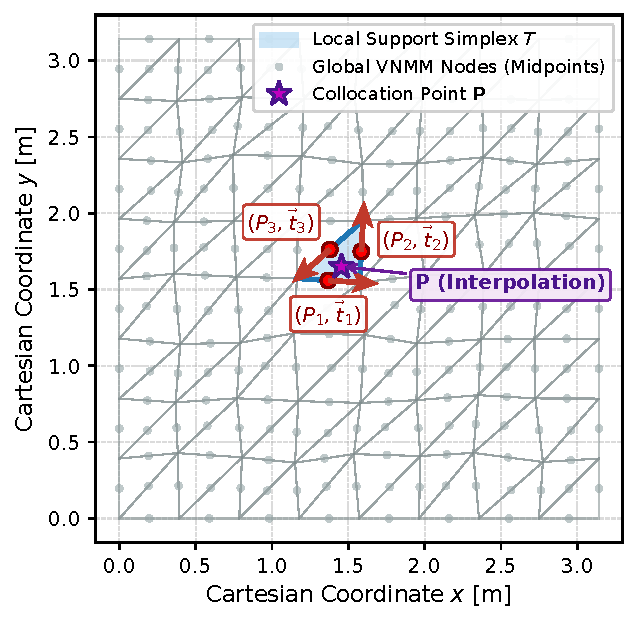
\includegraphics[width=0.52\linewidth]{figura_malha_conforme_vnmm_L1.pdf}
    \caption{Conforming dual topology for Whitney EFEM and VNMM $\mathcal{L}^1$ over $\Omega = [0, \pi]^2$. Underlying triangular mesh overlaid with dual vector nodes placed at edge midpoints $M_k$ with tangent directors $\vec{t}_k$.}
    \label{fig:malha_conforme_vnmm_L1}
\end{figure}

\subsubsection{Numerical Identity and Asymptotic Convergence Rates}
The asymptotic convergence behavior comparing the VNMM 2D $\mathcal{L}^1$ and Whitney EFEM formulations across the seven conforming mesh levels is presented in Fig.~\ref{fig:convergencia_efem_vs_vnmm_L1}.

As demonstrated in Fig.~\ref{fig:convergencia_efem_vs_vnmm_L1}a, the electric field RMS error, defined over the $M$ sampling points as
\begin{equation}
    \|\vec{E} - \vec{E}^h\|_{\mathrm{RMS}} = \sqrt{\frac{1}{M}\sum_{p=1}^M \|\vec{E}(\mathbf{x}_p) - \vec{E}^h(\mathbf{x}_p)\|_2^2},
    \label{eq:rms_error_def}
\end{equation}
displays an identical first-order asymptotic decay rate of $\mathcal{O}(h^{1.00})$ for both formulations. The point-by-point field difference between the two methods remains bounded by double-precision floating-point machine precision, satisfying $\|\vec{E}^{\mathrm{VNMM}} - \vec{E}^{\mathrm{EFEM}}\|_{\mathrm{RMS}} \le 1.6 \times 10^{-16}$.

Similarly, Fig.~\ref{fig:convergencia_efem_vs_vnmm_L1}b illustrates the curl operator RMS error $\|(\nabla \times \vec{E})_z - (\nabla \times \vec{E}^h)_z\|_{\mathrm{RMS}}$, which exhibits an identical fitted convergence rate of $\mathcal{O}(h^{0.96})$ for both formulations. The mutual curl field difference is likewise bounded by machine precision, satisfying $\|(\nabla \times \vec{E})^{\mathrm{VNMM}} - (\nabla \times \vec{E})^{\mathrm{EFEM}}\|_{\mathrm{RMS}} \le 2.5 \times 10^{-15}$. These log-log convergence curves empirically confirm the theoretical equivalence established by Theorem~\ref{thm:dual_equivalence} (Section~\ref{subsubsec:formal_proof_dual_whitney} and \ref{app:dual_whitney_proof}), establishing that under conforming midpoint/tangent placement on triangular cells, the VNMM 2D $\mathcal{L}^1$ formulation and Whitney edge finite elements reproduce identical discrete approximations down to double-precision floating-point roundoff.

\begin{figure}[!htbp]
    \centering
    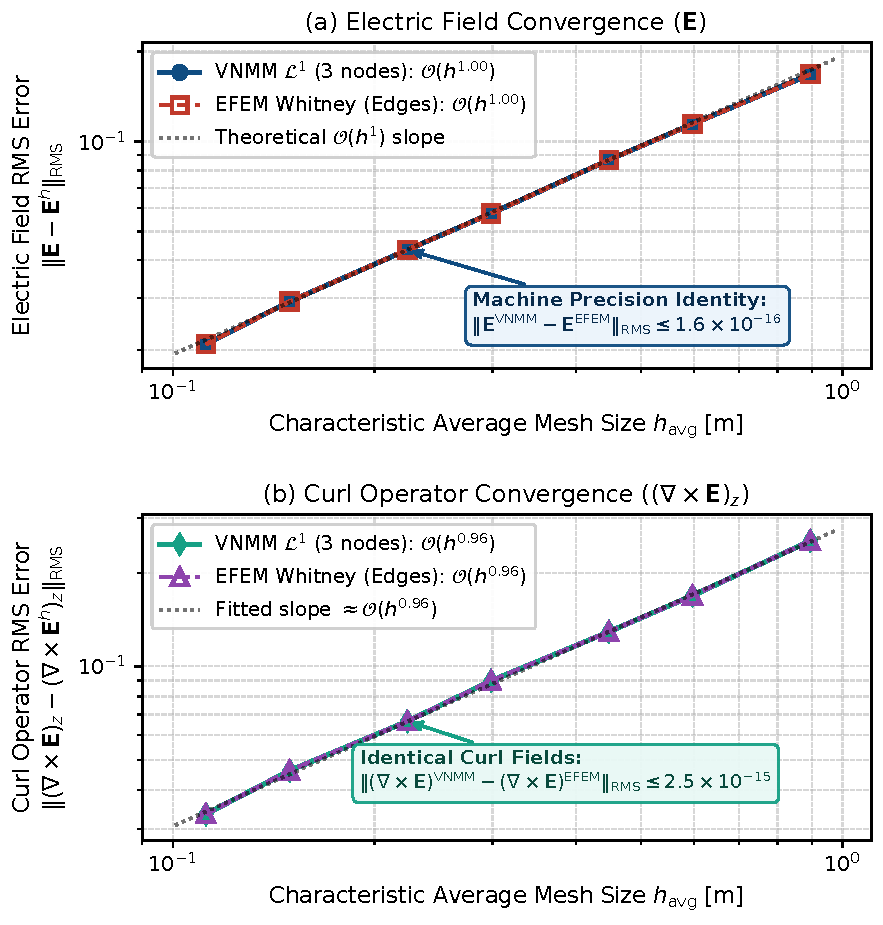
\includegraphics[width=0.62\linewidth]{figura_convergencia_efem_vs_vnmm_L1.pdf}
    \caption{Convergence comparison between Whitney EFEM and VNMM $\mathcal{L}^1$ on conforming triangular meshes.
        (a) Electric field RMS error $\|\vec{E} - \vec{E}^h\|_{\mathrm{RMS}}$ showing identical $\mathcal{O}(h^{1.00})$ convergence;
        (b) Curl operator RMS error displaying identical $\mathcal{O}(h^{0.96})$ convergence down to machine precision, confirming numerical identity.}
    \label{fig:convergencia_efem_vs_vnmm_L1}
\end{figure}

It should be noted that this machine-precision equivalence holds under conforming cell topologies where support triads match element midpoints with edge-tangent directors. On arbitrary point clouds, the VNMM ceases to be equivalent to a Whitney element, as arbitrary node coordinates, non-tangential director orientations, and dynamically shifting support stencils destroy simplex conformity, leading to the derivative stagnation examined next.


\subsection{Vector Field Interpolation and Derivative Convergence in Arbitrary Meshless Clouds}
\label{subsec:arbitrary_meshless_interpolation}

To evaluate performance in practical meshless settings where nodes do not coincide with triangulation midpoints, we assess convergence across unconstrained point distributions. This validates the modal aliasing analysis of Section~\ref{subsec:L1_aliasing_analysis} and confirms its resolution through the complete linear space $\mathcal{P}^1$.
\subsubsection{Experimental Setup on Unconstrained Point Clouds}
The interpolation performance is assessed for the analytical $TE_{11}$ cavity mode specified in Eq.~\eqref{eq:analytical_te11_field} over unstructured, non-conforming nodal distributions covering $\Omega = [0, \pi] \times [0, \pi]$. Boundary nodes are placed uniformly along the domain perimeter with counterclockwise unit tangent vectors, whereas internal nodes are generated following the baseline stochastic model with $25\%$ spatial jitter and uniform random director orientations (Table~\ref{tab:baseline_computational_setup}).

To ensure spatial evaluation consistency, all field and derivative errors are evaluated across a fixed, invariant Cartesian grid of $1{,}600$ internal sampling points ($40 \times 40$) distributed uniformly in $[0.04\pi, 0.96\pi]^2$. The computational domain is discretized over six refinement levels, with total node counts $N_{\mathrm{total}} \in \{84, 186, 416, 884, 1{,}928, 4{,}192\}$ and nominal unperturbed boundary spacings ranging from $h_{\mathrm{nom}} = 4\pi / N_{\mathrm{bnd}} = 0.5236$~m down to $0.0654$~m ($h_{\mathrm{nom}} \in \{0.52, 0.35, 0.22, 0.15, 0.10, 0.07\}$~m), where $N_{\mathrm{bnd}} \in \{24, 36, 56, 84, 128, 192\}$ denotes the number of boundary nodes along the perimeter $\partial\Omega$ of length $4\pi$.

\subsubsection{Empirical Validation of Curl Stagnation in \texorpdfstring{$\mathcal{L}^1$}{L1}}
\label{subsubsec:curl_stagnation_L1}
When evaluated on unconstrained meshless clouds, the 3-node solenoidal basis $\mathcal{L}^1$ exhibits the fundamental breakdown in derivative convergence predicted theoretically in Section~\ref{subsec:L1_aliasing_analysis}. As illustrated by the log-log curves in Fig.~\ref{fig:convergencia_interpolacao_L1_vs_P1}a, the electric field RMS error $\|\vec{E} - \vec{E}^h\|_{\mathrm{RMS}}$ under $\mathcal{L}^1$ decreases monotonically at a first-order rate of $\mathcal{O}(h^{0.97})$, dropping from $1.91 \times 10^{-1}$ ($h_{\mathrm{nom}} = 0.5236$~m) down to $2.46 \times 10^{-2}$ ($h_{\mathrm{nom}} = 0.0654$~m).

However, as revealed in Fig.~\ref{fig:convergencia_interpolacao_L1_vs_P1}b, the RMS error of the curl operator $\|(\nabla \times \vec{E})_z - (\nabla \times \vec{E}^h)_z\|_{\mathrm{RMS}}$ \textbf{stagnates at an $\mathcal{O}(1)$ error plateau} ($\approx 0.85$, varying between $8.33 \times 10^{-1}$ and $8.88 \times 10^{-1}$, asymptotic rate $\mathcal{O}(h^{-0.01}) \approx \mathcal{O}(1)$), failing to converge under spatial refinement ($N_{\mathrm{total}} = 4{,}192$). This persistent noise floor confirms the modal aliasing mechanism derived in Section~\ref{subsec:L1_aliasing_analysis}, wherein unrepresented normal field derivatives leak into the rotational coefficient via the inverted placement matrix $\mathbf{A}^{-1}$.
\begin{figure}[!htbp]
    \centering
    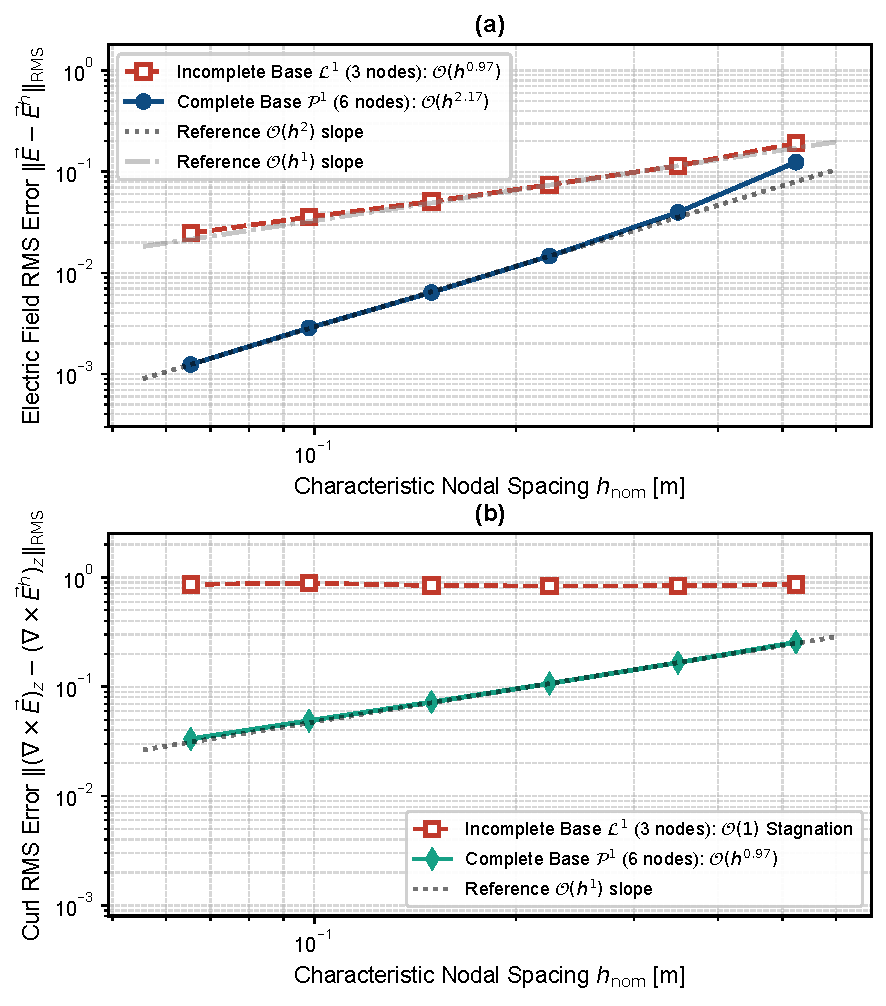
\includegraphics[width=0.62\linewidth]{figura_convergencia_interpolacao_L1_vs_P1.pdf}
    \caption{Convergence of $\mathcal{L}^1$ and $\mathcal{P}^1$ bases on unconstrained point clouds for the $TE_{11}$ mode.
        (a) Electric field RMS error showing $\mathcal{O}(h^{0.97})$ ($\mathcal{L}^1$) versus $\mathcal{O}(h^{2.17})$ ($\mathcal{P}^1$);
        (b) Curl operator RMS error highlighting $\mathcal{O}(1)$ stagnation for $\mathcal{L}^1$ and restored $\mathcal{O}(h^{0.97})$ convergence for $\mathcal{P}^1$.}
    \label{fig:convergencia_interpolacao_L1_vs_P1}
\end{figure}

\subsubsection{Restoration of Asymptotic Convergence via Complete \texorpdfstring{$\mathcal{P}^1$}{P1} Basis}
Expanding the local approximation space to the complete linear polynomial vector space $\mathcal{P}^1$ introduced in Section~\ref{subsec:complete_P1_basis} provides six independent degrees of freedom, capturing all four components of the local Jacobian tensor $\nabla\vec{E}^h$. Active support sextets are selected via the baseline scale-invariant pipeline ($h_{\mathrm{local}} = h_{\mathrm{nom}}$, $\widehat{\mathrm{Tol}} = 0.80$), yielding compact local stencils with $K_{\mathrm{avg}} \approx 10.7\text{--}11.2$ across all six refinement levels.

As demonstrated in Fig.~\ref{fig:convergencia_interpolacao_L1_vs_P1}, transitioning to $\mathcal{P}^1$ removes derivative modal aliasing and achieves two major performance gains:
\begin{enumerate}
    \item \textbf{Observed Convergence for Field $\vec{E}^h$ (Fig.~\ref{fig:convergencia_interpolacao_L1_vs_P1}a):} Completing the linear polynomial space elevates the observed electric field convergence rate from $\mathcal{O}(h^{0.97})$ under $\mathcal{L}^1$ to an observed fitted slope of $\mathcal{O}(h^{2.17})$ under $\mathcal{P}^1$. At the finest discretization ($h_{\mathrm{nom}} = 0.0654$~m), the field RMS error drops from $2.46 \times 10^{-2}$ ($\mathcal{L}^1$) down to $1.24 \times 10^{-3}$ ($\mathcal{P}^1$), representing a \textbf{$19.8\times$ precision gain}. This empirical convergence acceleration highlights the substantial accuracy benefit of resolving the complete local Jacobian, in contrast to the incomplete $\mathcal{L}^1$ formulation whose missing longitudinal polynomial terms restrict error reduction.
    \item \textbf{Restoration of Asymptotic $\mathcal{O}(h^1)$ Curl Convergence (Fig.~\ref{fig:convergencia_interpolacao_L1_vs_P1}b):} By accommodating normal derivatives in the Taylor expansion, the complete $\mathcal{P}^1$ basis restores first-order convergence $\mathcal{O}(h^{0.97})$ for the curl operator. The curl RMS error decreases monotonically from $2.55 \times 10^{-1}$ down to $3.33 \times 10^{-2}$ at $h_{\mathrm{nom}} = 0.0654$~m, delivering a \textbf{$25.9\times$ error reduction} over the stagnated $\mathcal{L}^1$ formulation ($8.63 \times 10^{-1}$).
\end{enumerate}

Consequently, while $\mathcal{L}^1$ is suitable for conforming triangular meshes where circulation cancellation holds (Section~\ref{subsec:conforming_dual_equivalence}), adopting the complete $\mathcal{P}^1$ vector space is sufficient to eliminate the derivative-aliasing mechanism and restore first-order curl convergence across unconstrained, arbitrary meshless point clouds. The quantitative performance comparison between the two bases across all six refinement levels is detailed in Table~\ref{tab:interpolacao_L1_vs_P1}.

\begin{table}[!htbp]
    \centering
    \caption{Comparative interpolation and curl error metrics between $\mathcal{L}^1$ and $\mathcal{P}^1$ bases on perturbed point clouds for the $TE_{11}$ mode across six refinement levels.}
    \label{tab:interpolacao_L1_vs_P1}
    \resizebox{\columnwidth}{!}{%
        \begin{tabular}{@{} c c c c c c c c c @{}}
            \toprule
            $N_{\mathrm{total}}$                     & $h_{\mathrm{nom}}$ [m]  & \multicolumn{3}{c}{\textbf{Electric Field RMS Error}} & \multicolumn{3}{c}{\textbf{Curl Operator RMS Error}} & $K_{\mathrm{avg}}$                                                                                                              \\
            \cmidrule(lr){3-5} \cmidrule(lr){6-8}
                                                     &                         & $\mathcal{L}^1$                                       & $\mathcal{P}^1$                                      & \textbf{Gain}            & $\mathcal{L}^1$                  & $\mathcal{P}^1$       & \textbf{Gain}         & ($\mathcal{P}^1$) \\
            \midrule
            84                                       & 0.5236                  & $1.91 \times 10^{-1}$                                 & $1.24 \times 10^{-1}$                                & $\mathbf{1.5\times}$     & $8.61 \times 10^{-1}$            & $2.55 \times 10^{-1}$ & $\mathbf{3.4\times}$  & 11.1              \\
            186                                      & 0.3491                  & $1.15 \times 10^{-1}$                                 & $3.97 \times 10^{-2}$                                & $\mathbf{2.9\times}$     & $8.38 \times 10^{-1}$            & $1.66 \times 10^{-1}$ & $\mathbf{5.0\times}$  & 11.2              \\
            416                                      & 0.2244                  & $7.44 \times 10^{-2}$                                 & $1.47 \times 10^{-2}$                                & $\mathbf{5.1\times}$     & $8.34 \times 10^{-1}$            & $1.07 \times 10^{-1}$ & $\mathbf{7.8\times}$  & 11.2              \\
            884                                      & 0.1496                  & $5.08 \times 10^{-2}$                                 & $6.39 \times 10^{-3}$                                & $\mathbf{7.9\times}$     & $8.43 \times 10^{-1}$            & $7.24 \times 10^{-2}$ & $\mathbf{11.6\times}$ & 10.9              \\
            1{,}928                                  & 0.0982                  & $3.56 \times 10^{-2}$                                 & $2.86 \times 10^{-3}$                                & $\mathbf{12.5\times}$    & $8.88 \times 10^{-1}$            & $4.89 \times 10^{-2}$ & $\mathbf{18.1\times}$ & 10.9              \\
            4{,}192                                  & 0.0654                  & $2.46 \times 10^{-2}$                                 & $1.24 \times 10^{-3}$                                & $\mathbf{19.8\times}$    & $8.63 \times 10^{-1}$            & $3.33 \times 10^{-2}$ & $\mathbf{25.9\times}$ & 10.7              \\
            \midrule
            \multicolumn{2}{c}{\textbf{Fitted Rate}} & $\mathcal{O}(h^{0.97})$ & $\mathbf{\mathcal{O}(h^{2.17})}$                      & ---                                                  & $\mathcal{O}(h^{-0.01})$ & $\mathbf{\mathcal{O}(h^{0.97})}$ & ---                   & ---                                       \\
            \bottomrule
        \end{tabular}%
    }
\end{table}

% ---------------------------------------------------------
% SUBSECTION 5.3: NUMERICAL STABILITY UNDER STOCHASTIC PERTURBATIONS
% ---------------------------------------------------------
\subsection{Numerical Robustness in the Tested Stochastic Realization Under Spatial-Directional Perturbations}
\label{subsec:stochastic_perturbations}

While Section~\ref{subsec:arbitrary_meshless_interpolation} adopted a fixed threshold ($\widehat{\mathrm{Tol}} = 0.80$) to demonstrate curl convergence restoration via $\mathcal{P}^1$, this section investigates how $\widehat{\mathrm{Tol}}$ governs stencil qualification, algebraic stability, and interpolation accuracy. On unconstrained point clouds with spatial and directional disorder, arbitrary arrangements can approach the null-space orthogonality singularity condition (Section~\ref{subsec:singularities_P1}), degrading the conditioning of $\mathbf{A} \in \mathbb{R}^{6 \times 6}$. Using the baseline stochastic cloud sequence (Table~\ref{tab:baseline_computational_setup}) across $N_{\mathrm{total}} = 84$ to $4{,}192$, we evaluate the performance across $\widehat{\mathrm{Tol}} \in [0.05, 6.00]$. Figure~\ref{fig:robustez_perturbacao_estocastica} and Table~\ref{tab:stochastic_sensitivity_ultradense} summarize the resulting convergence, conditioning, and parametric sensitivity.

\begin{figure}[!htbp]
    \centering
    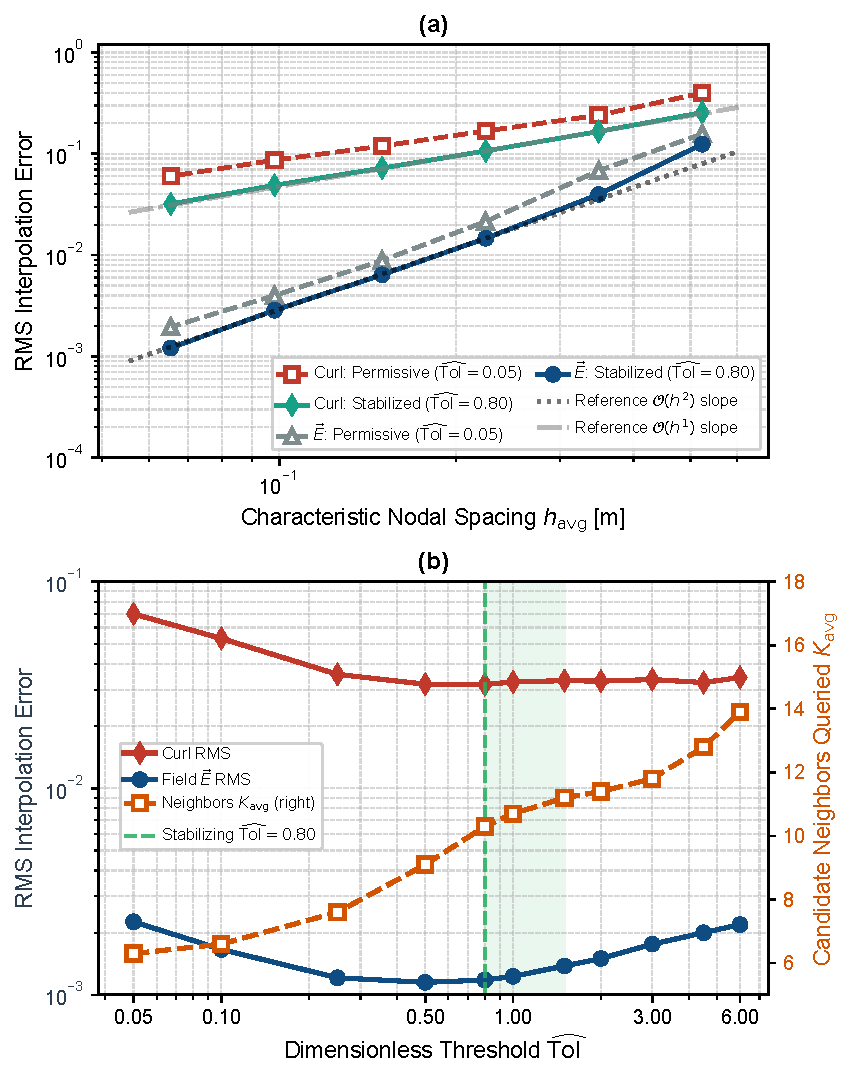
\includegraphics[width=0.62\linewidth]{figura_robustez_perturbacao_estocastica.pdf}
    \caption{Conditioning and robustness of the VNMM $\mathcal{P}^1$ basis under spatial-directional perturbations.
    (a) Electric field and curl RMS errors versus nominal spacing $h_{\mathrm{nom}}$, comparing a permissive threshold ($\widehat{\mathrm{Tol}} = 0.05$) against the calibrated threshold ($\widehat{\mathrm{Tol}} = 0.80$);
    (b) Error metrics and average support size $K_{\mathrm{avg}}$ versus $\widehat{\mathrm{Tol}}$ on the fine cloud ($N_{\mathrm{total}} = 4{,}192$), identifying the stable window $\widehat{\mathrm{Tol}} \in [0.80, 1.50]$.}
    \label{fig:robustez_perturbacao_estocastica}
\end{figure}

\subsubsection{Degradation Under Permissive Thresholds vs. Scale-Invariant Stabilization}
\label{subsubsec:permissive_threshold_degradation}

Under spatial-directional perturbations, an excessively relaxed threshold ($\widehat{\mathrm{Tol}} \le 0.05$) causes early-stopping qualification to accept immediate spatial neighbors ($K_{\mathrm{avg}} \approx 6.3$). Because these candidate stencils frequently approach the null-space orthogonality hypersurface of Section~\ref{subsec:singularities_P1}, the condition number inflates to $\kappa_2(\widehat{\mathbf{A}}) > 13$ (unscaled $\kappa_2(\mathbf{A}) > 180$). As spatial derivatives scale as $\mathcal{O}(h^{-1})$ via Eq.~\eqref{eq:curl_hat_eval}, the ill-conditioned inverse $\widehat{\mathbf{A}}^{-1}$ amplifies local errors, causing the curl RMS error to flatten into an error plateau ($\approx 6.0\times 10^{-2}$ to $8.7\times 10^{-2}$, dashed crimson curve in Fig.~\ref{fig:robustez_perturbacao_estocastica}a).

Enforcing a scale-invariant lower bound $\widehat{\mathrm{Tol}} \ge 0.80$ completely eliminates this instability. Candidate sextets approaching the null-space orthogonality singularity are systematically rejected, moderately expanding the search radius ($K_{\mathrm{avg}}$ expands from $6.3$ to $10.3$) to identify well-conditioned sextets with balanced angular diversity. As shown by the solid curves in Fig.~\ref{fig:robustez_perturbacao_estocastica}a, this restores monotonic convergence for both field $\vec{E}^h$ and curl $(\nabla \times \vec{E}^h)_z$, reducing fine-mesh curl error to $3.18 \times 10^{-2}$ on $N_{\mathrm{total}} = 4{,}192$. Because qualification operates on $\widehat{\mathbf{A}}$, the threshold $\widehat{\mathrm{Tol}}$ remains scale-invariant across all refinement levels, avoiding support dilation as $h \to 0$.

\subsubsection{Parametric Trade-off and Stable Operating Window}
\label{subsubsec:parametric_tradeoff}

To evaluate the sensitivity and identify a suitable operating regime, a parametric sweep was conducted on the fine cloud ($N_{\mathrm{total}} = 4{,}192$) for $\widehat{\mathrm{Tol}} \in [0.05, 6.00]$ (Table~\ref{tab:stochastic_sensitivity_ultradense} and Fig.~\ref{fig:robustez_perturbacao_estocastica}b). All $1{,}600$ evaluation points successfully identified admissible supports without search starvation across all thresholds.

As $\widehat{\mathrm{Tol}}$ increases from $0.05$ to $0.80$, the curl RMS error drops monotonically by $2.2\times$ ($6.98 \times 10^{-2} \to 3.18 \times 10^{-2}$), bounding conditioning to $\kappa_2(\widehat{\mathbf{A}}) \le 5.9$ with compact local stencils ($K_{\mathrm{avg}} = 10.3$). In the window $\widehat{\mathrm{Tol}} \in [0.80, 1.50]$, accuracy and conditioning remain stable ($K_{\mathrm{avg}} \le 11.2, \kappa_2 \le 5.9$). For $\widehat{\mathrm{Tol}} \ge 3.00$, conditioning improves marginally ($\kappa_2 \approx 3.3\text{--}4.0$) at the cost of broader support stencils ($K_{\mathrm{avg}} \to 13.9$ at $\widehat{\mathrm{Tol}} = 6.00$) and increased field interpolation errors ($+85\%$). Thus, $\widehat{\mathrm{Tol}} \in [0.80, 1.50]$ represents a well-balanced compromise between conditioning, locality, and precision.

\begin{table}[!htbp]
    \centering
    \small
    \caption{Sensitivity of error metrics, support neighborhood $K_{\mathrm{avg}}$, and conditioning to the dimensionless threshold $\widehat{\mathrm{Tol}}$ on the fine point cloud ($N_{\mathrm{total}} = 4{,}192$).}
    \label{tab:stochastic_sensitivity_ultradense}
    \resizebox{\columnwidth}{!}{%
        \begin{tabular}{@{} c c c c c @{}}
            \toprule
            \textbf{Dimensionless Threshold}                                                            & \textbf{Neighbors} & \multicolumn{2}{c}{\textbf{RMS Error}} & \textbf{Conditioning}                                                                                                                     \\
            \cmidrule(lr){3-4}
            $\widehat{\mathrm{Tol}}$                                                                    & $K_{\mathrm{avg}}$ & $\vec{E}^h$                            & $(\nabla\times\vec{E}^h)_z$    & $\kappa_2(\widehat{\mathbf{A}}) \; [\kappa_2(\mathbf{A})]$                                               \\
            \midrule
            \begin{tabular}[c]{@{}c@{}} 0.05 \\ \scriptsize(Permissive) \end{tabular}                   & 6.3                & $2.26 \times 10^{-3}$                  & $6.98 \times 10^{-2}$          & \begin{tabular}[c]{@{}c@{}} $\approx 13.4 \; [186]$ \\ \scriptsize(Ill-cond.) \end{tabular}              \\
            0.10                                                                                        & 6.6                & $1.66 \times 10^{-3}$                  & $5.31 \times 10^{-2}$          & $\approx 11.8 \; [162]$                                                                                  \\
            0.25                                                                                        & 7.6                & $1.21 \times 10^{-3}$                  & $3.56 \times 10^{-2}$          & $\approx 9.0 \; [124]$                                                                                   \\
            0.50                                                                                        & 9.1                & $1.15 \times 10^{-3}$                  & $3.19 \times 10^{-2}$          & $\approx 6.9 \; [94]$                                                                                    \\
            \begin{tabular}[c]{@{}c@{}} \textbf{0.80} \\ \scriptsize\textbf{(Stable)} \end{tabular}     & \textbf{10.3}      & $\mathbf{1.18 \times 10^{-3}}$         & $\mathbf{3.18 \times 10^{-2}}$ & \begin{tabular}[c]{@{}c@{}} $\mathbf{\approx 5.9 \; [80]}$ \\ \scriptsize\textbf{(Stable)} \end{tabular} \\
            1.00                                                                                        & 10.7               & $1.23 \times 10^{-3}$                  & $3.27 \times 10^{-2}$          & $\approx 5.6 \; [75]$                                                                                    \\
            \begin{tabular}[c]{@{}c@{}} \textbf{1.50} \\ \scriptsize\textbf{(Compromise)} \end{tabular} & \textbf{11.2}      & $\mathbf{1.38 \times 10^{-3}}$         & $\mathbf{3.32 \times 10^{-2}}$ & \begin{tabular}[c]{@{}c@{}} $\mathbf{\approx 5.1 \; [66]}$ \\ \scriptsize\textbf{(Stable)} \end{tabular} \\
            2.00                                                                                        & 11.4               & $1.50 \times 10^{-3}$                  & $3.30 \times 10^{-2}$          & $\approx 4.6 \; [59]$                                                                                    \\
            3.00                                                                                        & 11.8               & $1.76 \times 10^{-3}$                  & $3.36 \times 10^{-2}$          & $\approx 4.0 \; [50]$                                                                                    \\
            \begin{tabular}[c]{@{}c@{}} 6.00 \\ \scriptsize(Over-constrained) \end{tabular}             & 13.9               & $2.19 \times 10^{-3}$                  & $3.44 \times 10^{-2}$          & $\approx 3.3 \; [39]$                                                                                    \\
            \bottomrule
        \end{tabular}%
    }
\end{table}


% ---------------------------------------------------------
% ---------------------------------------------------------
% SUBSECTION 5.4: VARIATIONAL VERIFICATION: GALERKIN PATCH TEST AND METHOD OF MANUFACTURED SOLUTIONS
% ---------------------------------------------------------
\subsection{Variational Verification: Galerkin Patch Test and Method of Manufactured Solutions}
\label{subsec:patch_test_galerkin}

While Section~\ref{subsec:arbitrary_meshless_interpolation} established that the complete linear polynomial vector space $\mathcal{P}^1$ restores $\mathcal{O}(h^1)$ convergence in pointwise collocation, true convergence and numerical stability of a Ritz-Galerkin meshless formulation further demand \emph{linear completeness} and systematic asymptotic convergence in the presence of continuous differential operators \cite{belytschko1994element,liu2009mesh}. In this section, the discrete Galerkin operator is subjected to two complementary levels of numerical verification:
\begin{enumerate}
    \item \textbf{The Galerkin Patch Test:} Verifies that the global discrete operator reproduces arbitrary affine polynomial fields (with spatially constant curl and divergence) exactly to machine precision without discretization bias under inhomogeneous boundary conditions.
    \item \textbf{The Method of Manufactured Solutions (MMS):} Verifies the asymptotic convergence rates $\mathcal{O}(h^p)$ under spatial refinement ($h \to 0$) for a driven Maxwell/Helmholtz boundary value problem driven by a distributed volumetric source and spatially varying curl.
\end{enumerate}

\subsubsection{Part A: Galerkin Patch Test for Affine Vector Fields}
\label{subsubsec:patch_test_affine}

Consider an arbitrary affine 2D vector field:
\begin{equation}
    \vec{E}^*(\mathbf{x}) = \begin{bmatrix} a_1 + b_1 x + b_2 y \\[2pt] a_2 + b_3 x + b_4 y \end{bmatrix}, \quad a_i, b_i \in \mathbb{R}.
    \label{eq:affine_target_field}
\end{equation}
Because all first-order spatial derivatives of $\vec{E}^*$ are spatially constant across $\Omega$, its curl and divergence evaluate to invariant scalars:
\begin{equation}
    (\nabla \times \vec{E}^*)_z = b_3 - b_2 = C_{\mathrm{curl}}, \qquad \nabla \cdot \vec{E}^* = b_1 + b_4 = C_{\mathrm{div}}.
    \label{eq:patch_test_constants}
\end{equation}
Consequently, the physical vector PDE $\nabla \times \nabla \times \vec{E}^* - s_{\mathrm{div}} \nabla(\nabla \cdot \vec{E}^*) = \mathbf{0}$ is satisfied identically in $\Omega$. In the regularized Ritz-Galerkin weak form~\eqref{eq:regularized_weak_form}, the continuous bilinear form evaluated against any admissible test function $\vec{W} = \vec{N}_i$ yields the discrete load component:
\begin{equation}
    F_i \triangleq \int_\Omega \left[ \frac{1}{\mu_r} (\nabla \times \vec{N}_i)_z C_{\mathrm{curl}} + s_{\mathrm{div}} (\nabla \cdot \vec{N}_i) C_{\mathrm{div}} \right] d\Omega.
    \label{eq:patch_test_rhs}
\end{equation}
For any \emph{harmonic affine field} ($C_{\mathrm{curl}} = 0$ and $C_{\mathrm{div}} = 0$), $F_i \equiv 0$ identically, reducing the patch test to a pure homogeneous interior Dirichlet problem without external forcing.

To span the full 6-dimensional linear vector space $\mathcal{P}_1 \times \mathcal{P}_1$, we test seven canonical affine field configurations: (1) \textbf{Translation $X$:} $\vec{E}^* = [1, 0]^T$ (harmonic); (2) \textbf{Translation $Y$:} $\vec{E}^* = [0, 1]^T$ (harmonic); (3) \textbf{Normal Strain:} $\vec{E}^* = [x, -y]^T$ (harmonic); (4) \textbf{Shear Strain:} $\vec{E}^* = [y, x]^T$ (harmonic); (5) \textbf{Pure Curl:} $\vec{E}^* = [-y, x]^T$ ($C_{\mathrm{curl}} = 2, C_{\mathrm{div}} = 0$); (6) \textbf{Pure Divergence:} $\vec{E}^* = [x, y]^T$ ($C_{\mathrm{curl}} = 0, C_{\mathrm{div}} = 2$); and (7) \textbf{General Affine Field:} $\vec{E}^* = [1.5 + 0.8x - 0.3y, \; -0.7 + 0.4x + 1.2y]^T$ ($C_{\mathrm{curl}} = 0.7, C_{\mathrm{div}} = 2.0$).

The domain $\Omega = [0, \pi]^2$ is discretized using $N_x = N_y = 11$ ($N_{\mathrm{total}} = 121$ nodes, nominal spacing $h_{\mathrm{nom}} = \pi / 10 \approx 0.3142$~m). Boundary nodes ($N_{\mathrm{bnd}} = 40$) are placed along $\partial\Omega$ using the baseline staggered face-centered arrangement (Table~\ref{tab:baseline_computational_setup}), where exact Dirichlet degrees of freedom are imposed:
\begin{equation}
    e_k = \vec{E}^*(\mathbf{x}_k) \cdot \vec{t}_k, \quad \forall k \in \text{boundary nodes}.
    \label{eq:dirichlet_patch_imposition}
\end{equation}
The global linear system is partitioned into free interior degrees of freedom $\mathbf{e}_{\mathrm{int}} \in \mathbb{R}^{81}$ and prescribed boundary degrees of freedom $\mathbf{e}_{\mathrm{bnd}} \in \mathbb{R}^{40}$:
\begin{equation}
    \begin{bmatrix} \mathbf{K}_{\mathrm{int}, \mathrm{int}} & \mathbf{K}_{\mathrm{int}, \mathrm{bnd}} \\ \mathbf{K}_{\mathrm{bnd}, \mathrm{int}} & \mathbf{K}_{\mathrm{bnd}, \mathrm{bnd}} \end{bmatrix} \begin{bmatrix} \mathbf{e}_{\mathrm{int}} \\ \mathbf{e}_{\mathrm{bnd}} \end{bmatrix} = \begin{bmatrix} \mathbf{F}_{\mathrm{int}} \\ \mathbf{F}_{\mathrm{bnd}} \end{bmatrix} \implies \mathbf{K}_{\mathrm{int}, \mathrm{int}} \mathbf{e}_{\mathrm{int}} = \mathbf{F}_{\mathrm{int}} - \mathbf{K}_{\mathrm{int}, \mathrm{bnd}} \mathbf{e}_{\mathrm{bnd}}.
    \label{eq:patch_test_partitioned_system}
\end{equation}
To probe sensitivity to spatial irregularity, the patch test is solved on two contrasting nodal configurations: (i) a structured Cartesian grid with alternating internal directors; and (ii) an irregular cloud generated under the baseline stochastic model (both specified in Table~\ref{tab:baseline_computational_setup}).

\begin{table}[!htbp]
    \centering
    \small
    \caption{Galerkin patch test results: relative error in free interior degrees of freedom ($\|\mathbf{e}_{\mathrm{int}} - \mathbf{e}_{\mathrm{int}}^*\|_\infty / \|\mathbf{e}_{\mathrm{int}}^*\|_\infty$) comparing the complete $\mathcal{P}^1$ and incomplete $\mathcal{L}^1$ bases on structured and irregular point clouds ($121$ nodes, $81$ free interior DoFs, $s_{\mathrm{div}} = 6.0$).}
    \label{tab:galerkin_patch_test}
    \resizebox{\columnwidth}{!}{%
        \begin{tabular}{@{} l cccc @{}}
            \toprule
            \textbf{Affine Field Mode}                     & \multicolumn{2}{c}{\textbf{Regular Lattice}} & \multicolumn{2}{c}{\textbf{Irregular Cloud ($25\%$ Jitter)}}                                                         \\
            \cmidrule(lr){2-3} \cmidrule(lr){4-5}
                                                           & $\mathcal{P}^1$ Complete                     & $\mathcal{L}^1$ Incomplete                                   & $\mathcal{P}^1$ Complete & $\mathcal{L}^1$ Incomplete \\
            \midrule
            1. Translation $X$: $\vec{E} = [1, 0]^T$       & $4.49 \times 10^{-14}$                       & $3.93 \times 10^{-15}$                                       & $5.14 \times 10^{-14}$   & $1.34 \times 10^{-12}$     \\
            2. Translation $Y$: $\vec{E} = [0, 1]^T$       & $4.52 \times 10^{-14}$                       & $3.45 \times 10^{-15}$                                       & $7.38 \times 10^{-14}$   & $1.42 \times 10^{-12}$     \\
            3. Normal Strain: $\vec{E} = [x, -y]^T$        & $2.14 \times 10^{-14}$                       & $2.14 \times 10^{-1}$                                        & $5.07 \times 10^{-14}$   & $3.27 \times 10^{-1}$      \\
            4. Shear Strain: $\vec{E} = [y, x]^T$          & $2.78 \times 10^{-14}$                       & $1.51 \times 10^{-1}$                                        & $7.28 \times 10^{-14}$   & $4.69 \times 10^{-1}$      \\
            5. Pure Curl (Rotation): $\vec{E} = [-y, x]^T$ & $1.92 \times 10^{-14}$                       & $2.23 \times 10^{-15}$                                       & $1.25 \times 10^{-14}$   & $5.01 \times 10^{-13}$     \\
            6. Pure Divergence: $\vec{E} = [x, y]^T$       & $2.48 \times 10^{-14}$                       & $7.91 \times 10^{-2}$                                        & $5.45 \times 10^{-14}$   & $3.84 \times 10^{-1}$      \\
            7. Arbitrary General Affine Field              & $2.71 \times 10^{-14}$                       & $8.64 \times 10^{-2}$                                        & $5.25 \times 10^{-14}$   & $3.78 \times 10^{-1}$      \\
            \bottomrule
        \end{tabular}%
    }
\end{table}

Following standard patch-test conventions in meshless methods \cite{belytschko1994element,liu2009mesh}, Table~\ref{tab:galerkin_patch_test} compiles the discrete maximum nodal degree-of-freedom error ($\|\mathbf{e}_{\mathrm{int}} - \mathbf{e}_{\mathrm{int}}^*\|_\infty / \|\mathbf{e}_{\mathrm{int}}^*\|_\infty$) to verify that no individual interior node violates exact linear completeness. Inspection of the numerical results reveals two fundamental conclusions:
\begin{enumerate}
    \item \textbf{Linear Completeness and Patch-Test Satisfaction of $\mathcal{P}^1$:} For all seven affine modes on both regular and irregular point clouds, the complete linear vector basis $\mathcal{P}^1$ reproduces the exact interior degrees of freedom to double-precision machine precision ($\|\mathbf{e}_{\mathrm{int}} - \mathbf{e}_{\mathrm{int}}^*\|_\infty / \|\mathbf{e}_{\mathrm{int}}^*\|_\infty \le 7.38 \times 10^{-14}$). Furthermore, to verify continuous domain-wide fidelity beyond discrete nodes, evaluating the reconstructed solution across the background integration domain under $25\%$ spatial jitter and random directors confirms exact field and derivative reproduction in the continuous $L^2$ norm: the relative field error satisfies $\|\vec{E}^h - \vec{E}^*\|_{L^2} / \|\vec{E}^*\|_{L^2} \le 5.93 \times 10^{-14}$, the curl error satisfies $\|(\nabla \times \vec{E}^h)_z - C_{\mathrm{curl}}\|_{L^2} \le 1.92 \times 10^{-13}$, and the divergence error satisfies $\|\nabla \cdot \vec{E}^h - C_{\mathrm{div}}\|_{L^2} \le 8.37 \times 10^{-14}$. These results provide numerical verification that the complete basis $\mathcal{P}^1$, in conjunction with scale-invariant stencil qualification and regularized Ritz-Galerkin assembly, satisfies the Galerkin patch test to machine precision across all tested affine states.
    \item \textbf{Variational Breakdown of the Incomplete $\mathcal{L}^1$ Basis:} In contrast, the incomplete 3-node basis $\mathcal{L}^1$ passes the patch test only for rigid-body motions (Translations 1--2 and Rotation 5), which reside within its restricted solenoidal subspace. Notably, even for solenoidal and irrotational affine fields ($C_{\mathrm{curl}} = 0, C_{\mathrm{div}} = 0$), such as normal strain (Mode~3) and shear strain (Mode~4), $\mathcal{L}^1$ fails to reproduce the exact solution, exhibiting relative errors of $15.1\%\text{--}21.4\%$ on regular lattices and $32.7\%\text{--}46.9\%$ under spatial jitter. For the general affine field (Mode~7), $\mathcal{L}^1$ incurs an interior DoF error of $37.8\%$.
\end{enumerate}
This failure directly corroborates the theoretical analysis of Heuristic~\ref{heur:L1_aliasing}: on unconstrained point clouds lacking conforming closed-contour cancellation, the inability of $\mathcal{L}^1$ to represent normal and shear Jacobian gradients corrupts localized interpolation and contaminates the assembled Galerkin stiffness operator $\mathbf{K}_{\mathrm{curl}}$. Furthermore, because the $\mathcal{L}^1$ basis is solenoidal ($\nabla \cdot \vec{N}_i \equiv 0$), the divergence penalty operator vanishes identically ($\mathbf{K}_{\mathrm{div}} \equiv \mathbf{0}$), precluding variational div-curl regularization on this incomplete space.

\subsubsection{Part B: Driven Source Problem and Method of Manufactured Solutions (MMS)}
\label{subsubsec:mms_driven_problem}

While passing the patch test proves that the discrete Galerkin operator introduces no bias when the exact solution is affine, it does not probe the asymptotic rate of convergence when the solution possesses non-vanishing spatial curvature and inhomogeneous curl. To investigate the convergence rate of the Galerkin formulation under spatial refinement ($h \to 0$), we formulate a source-driven boundary value problem using the \textbf{Method of Manufactured Solutions} (MMS).

Consider the regularized vector Helmholtz equation posed on $\Omega = [0, \pi]^2$:
\begin{equation}
    \nabla \times \nabla \times \vec{E} - s_{\mathrm{div}} \nabla(\nabla \cdot \vec{E}) + \kappa \vec{E} = \vec{f}(\mathbf{x}) \quad \text{in } \Omega,
    \label{eq:mms_pde}
\end{equation}
subject to inhomogeneous essential Dirichlet conditions $\vec{E} \cdot \vec{t} = \vec{E}^* \cdot \vec{t}$ on $\partial\Omega$, with reaction parameter $\kappa = 1.0$ and divergence penalty parameter $s_{\mathrm{div}} = 6.0$. We prescribe the analytical solenoidal target field:
\begin{equation}
    \vec{E}^*(x, y) = \begin{bmatrix} \sin(x)\cos(y) \\[2pt] -\cos(x)\sin(y) \end{bmatrix}.
    \label{eq:mms_target_field}
\end{equation}
Direct analytical differentiation verifies that:
\begin{align}
    \nabla \cdot \vec{E}^*                  & \equiv 0, \qquad (\nabla \times \vec{E}^*)_z = 2\sin(x)\sin(y), \\
    \nabla \times (\nabla \times \vec{E}^*) & = 2\vec{E}^*.
\end{align}
By construction, on all four boundary segments of $\partial\Omega$ ($x \in \{0, \pi\}$ and $y \in \{0, \pi\}$), $\sin(x) = 0$ or $\sin(y) = 0$, implying that $(\nabla \times \vec{E}^*)_z = 0$ identically on $\partial\Omega$. Therefore, the natural boundary flux integral $\int_{\partial\Omega} (\vec{n} \times (\nabla \times \vec{E})) \cdot \vec{W}\, ds$ in the integration by parts vanishes identically. Substituting $\vec{E}^*$ into Eq.~\eqref{eq:mms_pde} yields the exact volumetric source distribution:
\begin{equation}
    \vec{f}(\mathbf{x}) = (2 + \kappa)\vec{E}^*(\mathbf{x}) = 3\vec{E}^*(\mathbf{x}).
    \label{eq:mms_source_term}
\end{equation}

In the Ritz-Galerkin discretization, the discrete system takes the form:
\begin{equation}
    \mathbf{A} \mathbf{e} = \mathbf{F}, \quad \text{with } \mathbf{A} = \mathbf{K}_{\mathrm{curl}} + s_{\mathrm{div}} \mathbf{K}_{\mathrm{div}} + \kappa \mathbf{M},
    \label{eq:mms_discrete_system}
\end{equation}
where $\mathbf{M}$ is the consistent vector mass matrix (Eq.~\eqref{eq:mass_matrix_entry} with $\epsilon_r = 1$), $\mathbf{K}_{\mathrm{curl}}$ and $\mathbf{K}_{\mathrm{div}}$ are the stiffness blocks defined in Eqs.~\eqref{eq:K_div_definition}--\eqref{eq:K_curl_definition}, and the load vector entries are defined by $F_i = \int_\Omega \vec{N}_i \cdot \vec{f}(\mathbf{x})\, d\Omega$. Prescribing Dirichlet boundary degrees of freedom $e_k = \vec{E}^*(\mathbf{x}_k) \cdot \vec{t}_k$ on $\partial\Omega$, the interior degrees of freedom are obtained from $\mathbf{A}_{\mathrm{int}, \mathrm{int}} \mathbf{e}_{\mathrm{int}} = \mathbf{F}_{\mathrm{int}} - \mathbf{A}_{\mathrm{int}, \mathrm{bnd}} \mathbf{e}_{\mathrm{bnd}}$. To quantify accuracy and asymptotic convergence under spatial refinement, the discrete solution is evaluated against the analytical field~\eqref{eq:mms_target_field} using three relative error metrics: the relative $L^2$ field error $\varepsilon_{L^2}(\vec{E}) = \|\vec{E}^h - \vec{E}^*\|_{L^2} / \|\vec{E}^*\|_{L^2}$, the relative curl semi-norm error $\varepsilon_{\mathrm{curl}}(\vec{E}) = \|(\nabla \times \vec{E}^h)_z - (\nabla \times \vec{E}^*)_z\|_{L^2} / \|(\nabla \times \vec{E}^*)_z\|_{L^2}$, and the maximum interior degree-of-freedom error $\varepsilon_{\mathrm{DoF}} = \|\mathbf{e}_{\mathrm{int}} - \mathbf{e}_{\mathrm{int}}^*\|_\infty / \|\mathbf{e}_{\mathrm{int}}^*\|_\infty$, while $\|\nabla \cdot \vec{E}^h\|_{L^2}$ tracks the domain divergence residual.

\begin{table}[!htbp]
    \centering
    \small
    \caption{Convergence of the Galerkin Method of Manufactured Solutions (MMS) under spatial refinement: relative $L^2$ field error, relative $H(\mathbf{curl})$ semi-norm error, maximum DoF error, and divergence residual comparing the complete $\mathcal{P}^1$ and incomplete $\mathcal{L}^1$ bases ($s_{\mathrm{div}} = 6.0$, $\kappa = 1.0$, $3 \times 3$ Gauss points per cell).}
    \label{tab:mms_convergence}
    \resizebox{\columnwidth}{!}{%
        \begin{tabular}{@{} c c c cccc c @{}}
            \toprule
            \textbf{Mesh Grid}                                                                            & \textbf{DoFs}        & $h_{\mathrm{nom}}$ [m] & \multicolumn{4}{c}{\textbf{Complete Basis $\mathcal{P}^1$}} & \textbf{Incomplete $\mathcal{L}^1$}                                                                                                       \\
            \cmidrule(lr){4-7} \cmidrule(lr){8-8}
            $N \times N$                                                                                  & $N_{\mathrm{total}}$ &                        & $\varepsilon_{L^2}(\vec{E})$                                & $\varepsilon_{\mathrm{curl}}(\vec{E})$ & $\varepsilon_{\mathrm{DoF}}$ & $\|\nabla \cdot \vec{E}^h\|_{L^2}$ & $\varepsilon_{L^2}(\vec{E})$ \\
            \midrule
            $9 \times 9$                                                                                  & 81                   & 0.3927                 & $12.32\%$                                                   & $29.05\%$                              & $23.74\%$                    & $4.24 \times 10^{-1}$              & $24.80\%$                    \\
            $13 \times 13$                                                                                & 169                  & 0.2618                 & $3.78\%$                                                    & $21.23\%$                              & $9.03\%$                     & $2.07 \times 10^{-1}$              & $24.15\%$                    \\
            $17 \times 17$                                                                                & 289                  & 0.1963                 & $1.85\%$                                                    & $14.75\%$                              & $5.70\%$                     & $1.29 \times 10^{-1}$              & $22.81\%$                    \\
            $21 \times 21$                                                                                & 441                  & 0.1571                 & $1.35\%$                                                    & $12.50\%$                              & $3.94\%$                     & $1.23 \times 10^{-1}$              & $25.91\%$                    \\
            $25 \times 25$                                                                                & 625                  & 0.1309                 & $1.34\%$                                                    & $17.47\%$                              & $4.75\%$                     & $1.11 \times 10^{-1}$              & $23.60\%$                    \\
            $29 \times 29$                                                                                & 841                  & 0.1122                 & $0.77\%$                                                    & $9.39\%$                               & $2.61\%$                     & $7.58 \times 10^{-2}$              & $23.87\%$                    \\
            \midrule
            \multicolumn{3}{@{}l}{\textbf{Empirical Convergence Rate $\mathcal{O}(h_{\mathrm{nom}}^p)$:}} & $\mathbf{p = 2.08}$  & $\mathbf{p = 0.75}$    & $\mathbf{p = 1.60}$                                         &                                        & $\mathbf{p = 0.02}$                                                                              \\
            \bottomrule
        \end{tabular}%
    }
\end{table}

We test a progressive refinement sequence of six regular lattices with $N \in \{9, 13, 17, 21, 25, 29\}$, spanning nominal nodal spacings from $h_{\mathrm{nom}} = 0.3927$~m down to $0.1122$~m ($81$ to $841$ degrees of freedom, with scale normalization $h_{\mathrm{local}} = h_{\mathrm{nom}}$). The numerical results are summarized in Table~\ref{tab:mms_convergence}. Two decisive phenomena emerge from this MMS convergence study:
\begin{enumerate}
    \item \textbf{Systematic Numerical Convergence for $\mathcal{P}^1$:} As the nodal spacing is refined, the complete $\mathcal{P}^1$ basis exhibits strict monotonic convergence in the $L^2$ field norm, reducing the relative error from $12.32\%$ on the coarsest mesh down to $0.77\%$ on $N = 29 \times 29$. A least-squares logarithmic regression yields an observed empirical convergence rate of $p = 2.08$ in the $L^2$ field norm, in close agreement with the theoretically expected $\mathcal{O}(h_{\mathrm{nom}}^2)$ rate for linear complete elements. Simultaneously, while standard approximation theory predicts an $\mathcal{O}(h^1)$ rate in $H(\mathbf{curl})$ for conforming spaces, the observed empirical slope in the present non-conforming meshless setting is $p = 0.75$ (dropping from $29.05\%$ to $9.39\%$). This sub-unitary slope reflects pre-asymptotic interaction between non-conforming support transitions and the divergence penalty operator. Although a mathematical proof of uniform convergence on arbitrary clouds remains an open question, these observed rates demonstrate that $\mathcal{P}^1$ overcomes the complete stagnation ($p = 0.02$) of the incomplete basis, while the discrete degree-of-freedom error decays as $\mathcal{O}(h_{\mathrm{nom}}^{1.60})$ and the divergence residual contracts by nearly an order of magnitude.
    \item \textbf{Convergence Stagnation of the Incomplete $\mathcal{L}^1$ Basis:} In stark contrast, the incomplete $\mathcal{L}^1$ basis fails to converge under refinement, exhibiting an asymptotic rate of $p = 0.02$. The relative $L^2$ field error remains trapped between $22.8\%$ and $25.9\%$, while the curl error hovers near $55\%\text{--}61\%$. Because the 3-node stencil $\mathcal{L}^1$ cannot represent normal derivative gradients on arbitrary node distributions, the discrete Galerkin stiffness operator cannot capture smooth vector field variations, leading to systematic stagnation regardless of grid refinement.
\end{enumerate}
Together with the patch test, these MMS results provide systematic numerical evidence that adopting the complete linear polynomial vector space $\mathcal{P}^1$ resolves the variational breakdown and convergence stagnation of the incomplete $\mathcal{L}^1$ basis, restoring systematic numerical convergence in Galerkin meshless discretizations, with observed rates aligning with expected polynomial behavior.


% ---------------------------------------------------------
% SUBSECTION 5.5: RESONANT CAVITY SPECTRAL ANALYSIS AND DIV-CURL REGULARIZATION
% ---------------------------------------------------------
\subsection{Spectral Validation: Resonant Cavity Analysis and Div-Curl Regularization}
\label{subsec:cavity_eigenvalues}
Having established the variational framework for the electromagnetic vector eigenvalue problem in Section~\ref{sec:variational_formulation}, this experiment evaluates the spectral accuracy of the Vector Nodal Meshless Method and verifies the shifting of non-physical spurious modes outside the operational frequency band. Numerical simulations are conducted for Transverse Electric ($TE_z$) modes over the square PEC cavity using the complete $\mathcal{P}^1$ basis, comparing discrete spectra against the analytical reference eigenvalues defined in Eq.~\eqref{eq:analytical_eigenvalues}.

Numerical evaluations are conducted on the base-case discretization with $N_x = N_y = 21$ ($N_{\mathrm{total}} = 441$ nodes, $N_{\mathrm{bnd}} = 80$, $N_{\mathrm{DoF}} = 361$ active internal degrees of freedom, $h_{\mathrm{nom}} = \pi/20 \approx 0.1571$~m) adhering to the baseline operational conventions established in Table~\ref{tab:baseline_computational_setup}: regular Cartesian coordinates, staggered face-centered boundary placement, checkerboard alternating internal directors, and a background Cartesian grid of $20 \times 20$ cells with $3 \times 3$ Gauss quadrature ($N_g = 3{,}600$, $N_g / N_{\mathrm{DoF}} \approx 10.0$).

Under the baseline qualification threshold ($\widehat{\mathrm{Tol}} = 0.80$), the geometric symmetry and orthogonal angular diversity of immediate neighbors generate well-conditioned placement matrices across all $3{,}600$ quadrature points (mean $|\det(\widehat{\mathbf{A}})| \approx 3.29$), yielding compact nearest-neighbor stencils ($K_{\mathrm{avg}} \approx 6.54$) that remain identically invariant for any $\widehat{\mathrm{Tol}} \le 1.00$. Homogeneous tangential PEC boundary conditions ($\vec{E}^h(\mathbf{x}_k) \cdot \vec{t}_k = 0$) are enforced via nodal elimination ($e_k = 0$).

\paragraph{Spectral Classification Protocol and Operational Bandwidth}
To ensure rigorous and consistent terminology across all spectral analyses, discrete eigenpairs $(\lambda_j, \mathbf{e}_j)$ are categorized according to the criteria defined in Section~\ref{subsec:weak_form_regularization}:
\begin{enumerate}
    \item \textbf{Operational Bandwidth ($\Lambda_{\mathrm{op}}$):} The frequency range of engineering interest is designated as $\Lambda_{\mathrm{op}} \triangleq (0, 10.0]$, which encompasses the first ten analytical physical resonances ($TE_{10}$ through $TE_{03}$, with exact eigenvalues $\lambda \in [1.0, 9.0]$).
    \item \textbf{Physical Modes:} Computed states in $\Lambda_{\mathrm{op}}$ that correlate with analytical $TE_{mn}$ field patterns and satisfy the solenoidal criterion $R_{\mathrm{div}}(\mathbf{e}_j) \ll 1$ (empirically $R_{\mathrm{div}} \le 1.65\%$, Table~\ref{tab:cavity_eigenvalues_base_case}).
    \item \textbf{Spurious (Gradient) Modes:} Non-physical states leaking from the discrete gradient nullspace ($\nabla_h \times \nabla_h \phi_h \neq \mathbf{0}$), identified by dominant irrotational energy ($R_{\mathrm{div}}(\mathbf{e}_j) \gg 1$, typically $> 10^3\%$). The spectrum is defined as purified within the operational bandwidth when the lowest spurious eigenvalue satisfies $\lambda_{\mathrm{spur}} > 10.0$.
\end{enumerate}

\subsubsection{Spectral Contamination in the Unregularized Curl-Curl Formulation (\texorpdfstring{$s_{\mathrm{div}} = 0.0$}{s(div) = 0.0})}
\label{subsubsec:unregularized_formulation}

As established in Section~\ref{subsec:weak_form_regularization}, meshless vector discretizations inherently lack discrete de Rham complex exactness due to global non-conformity ($V_h \not\subset H(\mathbf{curl})$), allowing discrete gradient fields to produce non-vanishing numerical curl residues ($\nabla_h \times \nabla_h \phi_h \neq \mathbf{0}$) at Gauss quadrature points. When solving the unregularized curl-curl formulation ($s_{\mathrm{div}} = 0.0$) on the base-case cavity ($N_x = N_y = 21$), this absence of an exact sequence triggers severe spectral contamination.

One might suspect that such spurious modes stem merely from numerical under-integration. However, evaluating the discrete operator $\mathbf{K}_{\mathrm{curl}}$ under the dense baseline quadrature ($20 \times 20$ cells, $3 \times 3$ Gauss points, $N_g / N_{\mathrm{DoF}} \approx 10.0$) rules out this hypothesis: the operator exhibits an empty discrete nullspace ($\dim\ker(\mathbf{K}_{\mathrm{curl}}) = 0$), proving that the Gauss points fully sample the discrete gradient field. Yet, because their numerical curl residues do not vanish, these unconstrained discrete gradient states leak directly into the positive spectrum, generating a dense ladder of non-physical spurious eigenvalues $\lambda \in (0.001, 0.90)$ below the fundamental physical resonance ($TE_{10}, \lambda = 1.0$).

The empirical impact of this nullspace leakage is illustrated in Fig.~\ref{fig:espectro_cavidade_regularizacao}a. Without volumetric divergence regularization ($s_{\mathrm{div}} = 0.0$), over $130$ non-physical gradient modes densely infiltrate the sub-resonance and operational spectrum ($\lambda \le 10$), completely corrupting analytical modal ordering and yielding massive cutoff wavenumber errors in the lowest discrete modes ($96.57\%$ in Table~\ref{tab:s_div_sensitivity}).

\begin{figure}[!htbp]
    \centering
    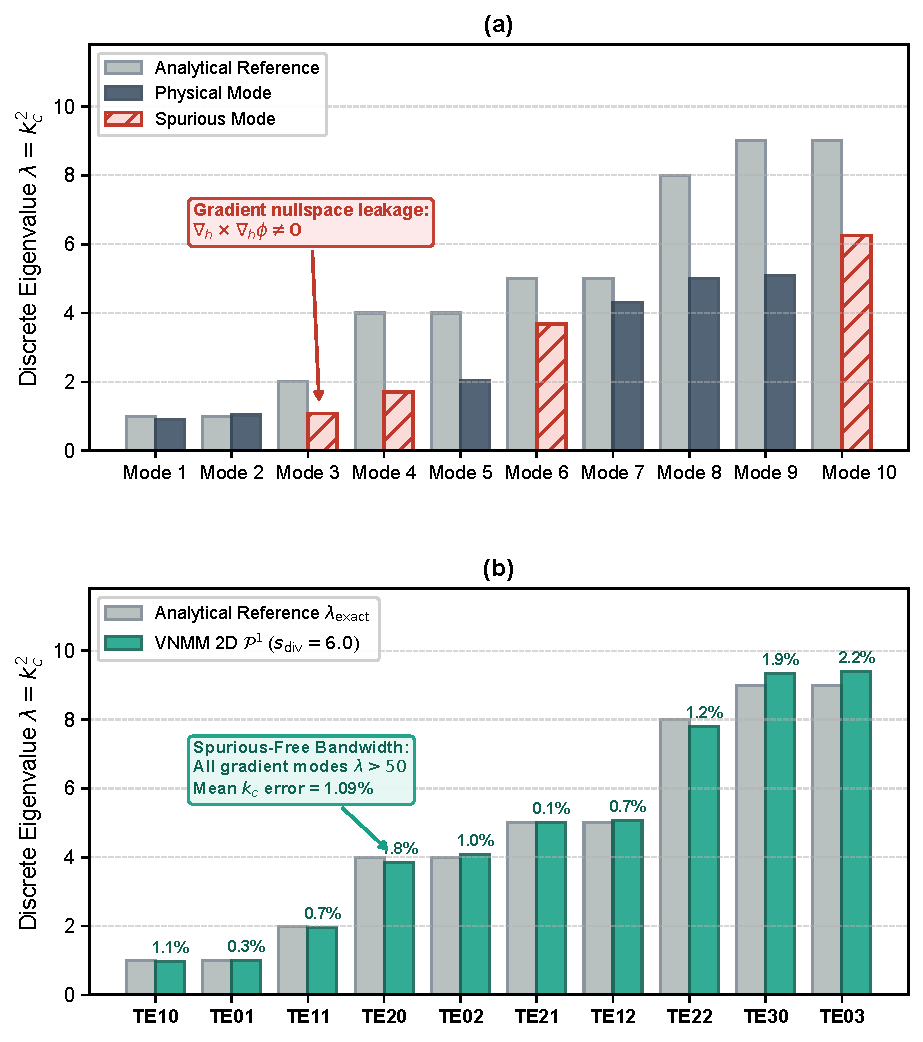
\includegraphics[width=0.62\linewidth]{figura_espectro_cavidade_com_sem_regularizacao.pdf}
    \caption{Discrete eigenvalue spectrum $\lambda = k_c^2$ for the $TE_z$ square PEC cavity.
        (a) Unregularized curl-curl formulation ($s_{\mathrm{div}} = 0.0$), showing spectral contamination from spurious gradient modes;
        (b) Div-curl regularized formulation ($s_{\mathrm{div}} = 6.0$), displaying a purified spectrum matching analytical modes within the operational bandwidth ($\lambda \le 10$).}
    \label{fig:espectro_cavidade_regularizacao}
\end{figure}

\subsubsection{Spectral Purification via Div-Curl Penalty Regularization (\texorpdfstring{$s_{\mathrm{div}} = 6.0$}{s(div) = 6.0})}
\label{subsubsec:regularized_formulation}

To shift the non-physical spurious gradient modes identified in Section~\ref{subsubsec:unregularized_formulation} outside the operational band without introducing auxiliary Lagrange multipliers or expanding the system matrix, the div-curl variational penalty parameter is activated with $s_{\mathrm{div}} = 6.0$ in Eq.~\eqref{eq:regularized_weak_form}. In accordance with the selective mechanism established in Section~\ref{subsec:weak_form_regularization}, this penalty selectively stiffens non-physical gradient states, shifting them past the 10th physical cavity mode ($\lambda_{\mathrm{spur}} = 11.84 > 10.37$), thereby clearing the operational spectrum of interest ($\lambda \le 10$) of detected non-physical states, while leaving solenoidal physical modes practically unaffected ($R_{\mathrm{div}} \le 1.65\%$). As analyzed in Section~\ref{subsubsec:s_div_sensitivity}, larger penalty parameters (such as $s_{\mathrm{div}} = 50.0$) can further elevate spurious modes to $\lambda_{\mathrm{spur}} > 50$, though at the expense of increased matrix conditioning and locking tendencies.

The experimental confirmation of this selective purification is demonstrated in Fig.~\ref{fig:espectro_cavidade_regularizacao}b. Activating $s_{\mathrm{div}} = 6.0$ ensures that no spurious modes are detected among the first ten computed resonances within the tested operational spectral window ($\lambda \le 10$), removing non-physical gradient branches from the low-frequency discrete spectrum and restoring 1-to-1 modal correspondence with the analytical reference eigenvalues defined in Eq.~\eqref{eq:analytical_eigenvalues}.

\subsubsection{Modewise Validation and Cutoff Wavenumber Precision}
\label{subsubsec:modewise_validation}

The numerical performance of the regularized VNMM 2D ($\mathcal{P}^1$, $s_{\mathrm{div}} = 6.0$, $\widehat{\mathrm{Tol}} = 0.80$) for the first 10 physical $TE_{nm}$ cavity modes is detailed in Table~\ref{tab:cavity_eigenvalues_base_case}.

\begin{table}[!htbp]
    \centering
    \caption{Comparison of the first 10 physical $TE_{nm}$ resonant modes in the square PEC cavity against analytical references ($361$ active DoFs, $20 \times 20$ cells, $3 \times 3$ Gauss points).}
    \label{tab:cavity_eigenvalues_base_case}
    \resizebox{\columnwidth}{!}{%
        \begin{tabular}{@{} c c c c c c c c @{}}
            \toprule
            \textbf{Mode ($TE_{nm}$)} & $\lambda_{\mathrm{analytical}}$ & $k_{c, \mathrm{analytical}}$ & $\lambda_{\mathrm{VNMM}}$ & $k_{c, \mathrm{VNMM}}$ & \textbf{Error $\lambda$ (\%)} & \textbf{Error $k_c$ (\%)} & $R_{\mathrm{div}}$ (\%) \\
            \midrule
            $TE_{10}$                 & $1.00$                          & $1.000$                      & $1.0081$                  & $1.004$                & $0.81\%$                      & $\mathbf{0.41\%}$         & $0.22\%$                \\
            $TE_{01}$                 & $1.00$                          & $1.000$                      & $1.0111$                  & $1.006$                & $1.11\%$                      & $\mathbf{0.55\%}$         & $0.21\%$                \\
            $TE_{11}$                 & $2.00$                          & $1.414$                      & $2.0809$                  & $1.443$                & $4.05\%$                      & $\mathbf{2.00\%}$         & $0.71\%$                \\
            $TE_{20}$                 & $4.00$                          & $2.000$                      & $4.2292$                  & $2.057$                & $5.73\%$                      & $\mathbf{2.83\%}$         & $0.66\%$                \\
            $TE_{02}$                 & $4.00$                          & $2.000$                      & $4.2505$                  & $2.062$                & $6.26\%$                      & $\mathbf{3.08\%}$         & $0.70\%$                \\
            $TE_{21}$                 & $5.00$                          & $2.236$                      & $5.5033$                  & $2.346$                & $10.07\%$                     & $\mathbf{4.91\%}$         & $1.30\%$                \\
            $TE_{12}$                 & $5.00$                          & $2.236$                      & $5.5255$                  & $2.351$                & $10.51\%$                     & $\mathbf{5.12\%}$         & $1.50\%$                \\
            $TE_{22}$                 & $8.00$                          & $2.828$                      & $9.1432$                  & $3.024$                & $14.29\%$                     & $\mathbf{6.91\%}$         & $1.65\%$                \\
            $TE_{30}$                 & $9.00$                          & $3.000$                      & $10.2889$                 & $3.208$                & $14.32\%$                     & $\mathbf{6.92\%}$         & $1.33\%$                \\
            $TE_{03}$                 & $9.00$                          & $3.000$                      & $10.3671$                 & $3.220$                & $15.19\%$                     & $\mathbf{7.33\%}$         & $1.46\%$                \\
            \midrule
            \textbf{Global Mean}      & ---                             & ---                          & ---                       & ---                    & $\mathbf{8.23\%}$             & $\mathbf{4.01\%}$         & $\mathbf{0.92\%}$       \\
            \bottomrule
        \end{tabular}%
    }
\end{table}

The regularized VNMM 2D achieves a global mean cutoff wavenumber error of $4.01\%$ (maximum $7.33\%$ for $TE_{03}$), preserving analytical degenerate pairings ($TE_{10}/TE_{01}$, $TE_{20}/TE_{02}$, $TE_{21}/TE_{12}$, $TE_{30}/TE_{03}$) with minor directional splitting ($\le 0.5\%$) from the alternating director lattice and zero spurious modes in the operational band ($\lambda \le 10$).

As reported in the final column of Table~\ref{tab:cavity_eigenvalues_base_case}, the discrete divergence-to-curl energy quotient $R_{\mathrm{div}}$ remains bounded between $0.21\%$ and $1.65\%$ (mean $0.92\% \ll 1$), confirming that physical modes incur negligible penalty stiffening. In contrast, unregularized gradient modes exhibit $R_{\mathrm{div}} \sim 10^3\%\text{--}10^6\%$; activating $s_{\mathrm{div}} = 6.0$ selectively elevates these states ($\lambda_{\mathrm{spur}} \ge 11.84$), shifting them past the tenth physical mode while leaving physical resonances unperturbed.

\subsubsection{Parametric Sensitivity to the Div-Curl Penalty Parameter (\texorpdfstring{$s_{\mathrm{div}}$}{s(div)})}
\label{subsubsec:s_div_sensitivity}

Table~\ref{tab:s_div_sensitivity} details the spectral response of the base cavity discretization ($N_x \times N_y = 21 \times 21$, $361$ active DoFs) across penalty values $s_{\mathrm{div}} \in [0.0, 50.0]$, delineating three distinct regimes:
\begin{enumerate}
    \item \textbf{Under-Penalization ($s_{\mathrm{div}} < 6.0$):} Unregularized formulation ($s_{\mathrm{div}} = 0.0$) suffers static gradient nullspace leakage, contaminating the spectrum with spurious modes ($\lambda \sim 10^{-3}$). Increasing $s_{\mathrm{div}}$ stiffens these branches, shifting $\lambda_{\mathrm{spur}}$ upward ($0.00 \to 7.93$).
    \item \textbf{Calibrated Operating Window ($s_{\mathrm{div}} \in [6.0, 10.0]$):} At $s_{\mathrm{div}} = 6.0$, the lowest spurious eigenvalue shifts beyond the tenth physical cavity mode ($\lambda_{\mathrm{spur}} = 11.84 > 10.37$). No spurious modes contaminate the operational window ($\lambda \le 10$), maintaining well-conditioned matrices ($\mathrm{cond}_2 \sim 3 \times 10^3$) and bounded divergence residuals ($R_{\mathrm{div}} \le 1.65\%$).
    \item \textbf{Over-Penalization ($s_{\mathrm{div}} > 10.0$):} Excessive penalization amplifies discrete divergence residuals ($\nabla \cdot \vec{E}^h \sim \mathcal{O}(h)$), inducing volumetric stiffening, modest accuracy loss ($4.01\% \to 18.50\%$), and elevated conditioning ($\mathrm{cond}_2 \sim 2.3 \times 10^4$ at $s_{\mathrm{div}} = 50.0$).
\end{enumerate}

\begin{table}[!htbp]
    \centering
    \small
    \caption{Parametric sensitivity of cavity spectral purity, cutoff wavenumber error, and stiffness matrix conditioning to the div-curl penalty parameter $s_{\mathrm{div}}$ ($361$ active DoFs, $20 \times 20$ cells, $3 \times 3$ Gauss points).}
    \label{tab:s_div_sensitivity}
    \resizebox{\columnwidth}{!}{%
        \begin{tabular}{@{} c c c c c c c @{}}
            \toprule
            $s_{\mathrm{div}}$ & \textbf{Spurious Modes}     & \textbf{Lowest Spurious}                        & \multicolumn{2}{c}{\textbf{Cutoff Error $k_c$}} & $\mathrm{cond}_2(\mathbf{K}_{\mathrm{red}})$ & \textbf{Max $R_{\mathrm{div}}$}                          \\
            \cmidrule(lr){4-5}
                               & \textbf{in Band ($\le 10$)} & \textbf{Eigenvalue ($\lambda_{\mathrm{spur}}$)} & \textbf{Mean (\%)}                              & \textbf{Max (\%)}                            &                                 & \textbf{Physical (\%)} \\
            \midrule
            $0.0$              & $10$                        & $0.00$                                          & $96.57\%$                                       & $97.20\%$                                    & $3.10 \times 10^5$              & ---                    \\
            $1.0$              & $5$                         & $1.99$                                          & $11.13\%$                                       & $29.38\%$                                    & $7.31 \times 10^2$              & $9.09\%$               \\
            $2.0$              & $1$                         & $3.98$                                          & $3.94\%$                                        & $19.33\%$                                    & $1.21 \times 10^3$              & $2.78\%$               \\
            $4.0$              & $1$                         & $7.93$                                          & $2.03\%$                                        & $5.55\%$                                     & $2.15 \times 10^3$              & $1.98\%$               \\
            $6.0$              & $\mathbf{0}$                & $\mathbf{11.84}$                                & $\mathbf{4.01\%}$                               & $\mathbf{7.33\%}$                            & $3.09 \times 10^3$              & $\mathbf{1.65\%}$      \\
            $8.0$              & $0$                         & $15.78$                                         & $4.92\%$                                        & $8.72\%$                                     & $4.03 \times 10^3$              & $1.45\%$               \\
            $10.0$             & $0$                         & $19.67$                                         & $5.78\%$                                        & $10.03\%$                                    & $4.96 \times 10^3$              & $1.36\%$               \\
            $20.0$             & $0$                         & $38.97$                                         & $9.54\%$                                        & $15.92\%$                                    & $9.54 \times 10^3$              & $1.22\%$               \\
            $50.0$             & $0$                         & $> 50$                                          & $18.50\%$                                       & $29.67\%$                                    & $2.26 \times 10^4$              & $1.03\%$               \\
            \bottomrule
        \end{tabular}%
    }
\end{table}

\paragraph{Theoretical Scaling and A Priori Calibration Criterion for $s_{\mathrm{div}}$}
The scaling of the lowest spurious eigenvalue can be directly derived from the continuous regularized variational problem~\eqref{eq:regularized_weak_form}. For pure gradient fields $\vec{E} = \nabla\phi$ with homogeneous tangential Dirichlet conditions ($\phi = 0$ on $\partial\Omega$), the curl vanishes identically ($\nabla \times \vec{E} \equiv \mathbf{0}$), reducing the continuous regularized operator to:
\begin{equation}
    -s_{\mathrm{div}}\nabla(\nabla \cdot \vec{E}) = -s_{\mathrm{div}}\nabla(\nabla^2\phi) = s_{\mathrm{div}}\mu \nabla\phi = s_{\mathrm{div}}\mu \vec{E},
    \label{eq:analytical_spurious_scaling}
\end{equation}
where $\mu$ denotes the eigenvalues of the scalar Dirichlet Laplacian ($-\nabla^2\phi = \mu\phi$ in $\Omega$, $\phi=0$ on $\partial\Omega$). For the square cavity $\Omega = [0, \pi]^2$, the Dirichlet Laplacian eigenvalues are $\mu_{m,n} = m^2 + n^2$ ($m,n \ge 1$), with the fundamental eigenvalue $\mu_{1,1} = 2.0$. Consequently, the lowest non-trivial gradient mode scales analytically as:
\begin{equation}
    \lambda_{\mathrm{spur}} \approx \mu_1 \cdot s_{\mathrm{div}} = 2.0 \cdot s_{\mathrm{div}}.
    \label{eq:spurious_eigenvalue_estimate}
\end{equation}
Under the resolution-matched baseline quadrature ($20 \times 20$ cells, $3 \times 3$ Gauss points), numerical evaluation confirms this scaling law down to $1.3\%$ error ($\lambda_{\mathrm{spur}}/s_{\mathrm{div}} \approx 1.97\text{--}1.99$).

Equation~\eqref{eq:spurious_eigenvalue_estimate} provides a predictive \emph{a priori} calibration rule: ensuring complete spectral clearance up to a target physical eigenvalue $\lambda_{\max}$ (here $\lambda_{\max} \approx 10.4$ for the first 10 cavity modes) requires:
\begin{equation}
    s_{\mathrm{div}} > \frac{\lambda_{\max}}{\mu_1} = \frac{10.4}{2.0} = 5.2,
    \label{eq:a_priori_s_div_rule}
\end{equation}
justifying the calibrated threshold $s_{\mathrm{div}} \ge 6.0$ from continuous operator theory.

\subsubsection{Sensitivity to Background Cell Density and Gauss Quadrature Order}
\label{subsubsec:quadrature_sensitivity}

To assess quadrature dependency, Table~\ref{tab:quadrature_sensitivity} reports the sensitivity across background grid densities and Gauss orders for the base cavity ($361$ active DoFs) compared to an ultra-refined reference ($40 \times 40$ cells, $4 \times 4$ Gauss points, $N_g = 25{,}600$).

\begin{table}[!htbp]
    \centering
    \small
    \caption{Sensitivity of cavity spectral accuracy, discrete matrix operators, and assembly time to background cell density and Gauss quadrature order ($361$ active DoFs).}
    \label{tab:quadrature_sensitivity}
    \resizebox{\columnwidth}{!}{%
        \begin{tabular}{@{} c c c c c c c c @{}}
            \toprule
            \textbf{Background Grid}      & \textbf{Gauss Rule}     & \textbf{Gauss Pts} & \multicolumn{2}{c}{\textbf{Wavenumber Error}} & \multicolumn{2}{c}{\textbf{Relative Matrix Difference}} & \textbf{Assembly}                                                                                                                                                                                             \\
            \cmidrule(lr){4-5} \cmidrule(lr){6-7}
            ($N_{cx} \times N_{cy}$)      & ($p \times p$)          & ($N_g$)            & \textbf{Mean $k_c$ (\%)}                      & \textbf{Max $k_c$ (\%)}                                 & $\frac{\|\mathbf{K} - \mathbf{K}_{\mathrm{ref}}\|_F}{\|\mathbf{K}_{\mathrm{ref}}\|_F}$ & $\frac{\|\mathbf{M} - \mathbf{M}_{\mathrm{ref}}\|_F}{\|\mathbf{M}_{\mathrm{ref}}\|_F}$ & \textbf{Time (s)}           \\
            \midrule
            $10 \times 10$ ($100$ cells)  & $2 \times 2$ ($4$ pts)  & $400$              & $\mathbf{1.09\%}$                             & $\mathbf{2.16\%}$                                       & $1.36 \times 10^0$                                                                     & $9.33 \times 10^{-1}$                                                                  & $\mathbf{0.02\,\mathrm{s}}$ \\
            $10 \times 10$ ($100$ cells)  & $3 \times 3$ ($9$ pts)  & $900$              & $1.65\%$                                      & $4.78\%$                                                & $5.22 \times 10^{-1}$                                                                  & $4.18 \times 10^{-1}$                                                                  & $0.06\,\mathrm{s}$          \\
            $10 \times 10$ ($100$ cells)  & $4 \times 4$ ($16$ pts) & $1600$             & $2.29\%$                                      & $5.93\%$                                                & $4.17 \times 10^{-1}$                                                                  & $4.65 \times 10^{-1}$                                                                  & $0.09\,\mathrm{s}$          \\
            \midrule
            $20 \times 20$ ($400$ cells)  & $2 \times 2$ ($4$ pts)  & $1600$             & $2.35\%$                                      & $5.97\%$                                                & $3.16 \times 10^{-1}$                                                                  & $3.65 \times 10^{-1}$                                                                  & $0.08\,\mathrm{s}$          \\
            $20 \times 20$ ($400$ cells)  & $4 \times 4$ ($16$ pts) & $6400$             & $2.82\%$                                      & $6.31\%$                                                & $8.42 \times 10^{-2}$                                                                  & $5.31 \times 10^{-2}$                                                                  & $0.36\,\mathrm{s}$          \\
            \midrule
            $30 \times 30$ ($900$ cells)  & $4 \times 4$ ($16$ pts) & $14400$            & $2.66\%$                                      & $5.80\%$                                                & $8.87 \times 10^{-2}$                                                                  & $1.03 \times 10^{-1}$                                                                  & $0.83\,\mathrm{s}$          \\
            $40 \times 40$ ($1600$ cells) & $2 \times 2$ ($4$ pts)  & $6400$             & $2.78\%$                                      & $6.07\%$                                                & $7.20 \times 10^{-2}$                                                                  & $5.95 \times 10^{-2}$                                                                  & $0.36\,\mathrm{s}$          \\
            $40 \times 40$ ($1600$ cells) & $4 \times 4$ ($16$ pts) & $25600$            & $2.94\%$                                      & $6.05\%$                                                & Reference                                                                              & Reference                                                                              & $1.55\,\mathrm{s}$          \\
            \bottomrule
        \end{tabular}%
    }
\end{table}

The results in Table~\ref{tab:quadrature_sensitivity} clarify the interaction between background quadrature and spatial discretization error, providing a cautionary pedagogical case study for non-conforming meshless methods. On coarse under-integrated grids ($10 \times 10, 2 \times 2$, $N_g / N_{\mathrm{DoF}} \approx 1.11$), numerical softening across intra-cell stencil transitions shifts discrete eigenvalues downward. This softening partially cancels the positive spatial discretization stiffening ($\lambda > \lambda_{\mathrm{exact}}$), producing an artificially low, deceptive error of $1.09\%$ that masks a severe $140$-dimensional numerical kernel defect in $\mathbf{K}_{\mathrm{curl}}$. Refining the background integration eliminates this artificial softening and restores full numerical rank ($\dim\ker(\mathbf{K}_{\mathrm{curl}}) = 0$), yielding a consistent baseline spatial discretization error of $4.01\%$ for cutoff wavenumbers ($0.41\%\text{--}7.33\%$ across the first 10 physical modes, Table~\ref{tab:cavity_eigenvalues_base_case}), which serves as the benchmark configuration reported throughout this paper. Consequently, the resolution-matched convention ($N_{cx} = N_{cy} = N_v - 1, 3 \times 3$ Gauss points, $N_g / N_{\mathrm{DoF}} \approx 10$, with cell spacing $h_{\mathrm{cell}} = h_{\mathrm{nom}}$) is adopted throughout all multi-level refinement and irregular cloud campaigns (Sections~\ref{subsec:convergence_comparison} and \ref{subsec:spectral_irregular_clouds}), ensuring that observed convergence rates reflect genuine vector basis approximation rather than quadrature artifacts.

% ---------------------------------------------------------
% SUBSECTION 5.5: COMPARATIVE CONVERGENCE: PURE VNMM 2D VS. EDGE FEM
% ---------------------------------------------------------
\subsection{Comparative Convergence: Pure VNMM 2D vs. Edge FEM}
\label{subsec:convergence_comparison}

To evaluate the numerical convergence behavior of the proposed Vector Nodal Meshless Method against the canonical standard in computational electromagnetics, this section evaluates the resonant frequencies of the Transverse Electric ($TE_z$) cavity across six successive discretization levels over $\Omega = [0, \pi]^2$:
\begin{enumerate}
    \item \textbf{Pure Edge FEM (Whitney 1-Forms):} Canonical conforming finite element solver on structured triangular meshes \cite{monk2003finite}, associating one circuital degree of freedom with each interior edge ($N_{\mathrm{DoF}} = N_{\mathrm{edges, int}}$).
    \item \textbf{Pure VNMM 2D ($\mathcal{P}^1$ Complete Basis):} Meshless solver over $\Omega$ configured under the baseline operational conventions established in Table~\ref{tab:baseline_computational_setup}: nominal spacing $h_{\mathrm{nom}} = \pi / (N_v - 1)$, staggered boundary nodes, alternating directors, $s_{\mathrm{div}} = 6.0$, $\widehat{\mathrm{Tol}} = 0.80$, and baseline $3 \times 3$ Gauss quadrature ($N_g / N_{\mathrm{DoF}} \approx 10$, $K_{\mathrm{avg}} \approx 6.5$).
\end{enumerate}

\subsubsection{Resolution Metric and Degree-of-Freedom Equivalence}
In a two-dimensional structured triangular mesh, Euler's planar graph formula yields \cite{deberg2008computational}:
\begin{equation}
    E \approx 3V,
    \label{eq:euler_edge_vertex}
\end{equation}
producing $N_{\mathrm{DoF}} \approx 3(N-1)^2$ for an $N \times N$ vertex Edge FEM mesh, whereas VNMM assigns one degree of freedom per internal node ($N_{\mathrm{DoF}} = (N_v - 2)^2 \approx V$). To ensure a fair comparison with matching DoF density ($\rho_{\mathrm{node}} \approx \rho_{\mathrm{edge}}$), we define the edge-equivalent nodal discretization parameter:
\begin{equation}
    N_v = \operatorname{round}\bigl(\sqrt{3}\,(N - 1)\bigr) + 1,
    \label{eq:edge_equivalent_nv}
\end{equation}
and track convergence as a function of the characteristic degree-of-freedom spacing:
\begin{equation}
    h_{\mathrm{DoF}} = \sqrt{\frac{|\Omega|}{N_{\mathrm{DoF}}}}.
    \label{eq:h_dof_definition}
\end{equation}

\begin{figure}[!htbp]
    \centering
    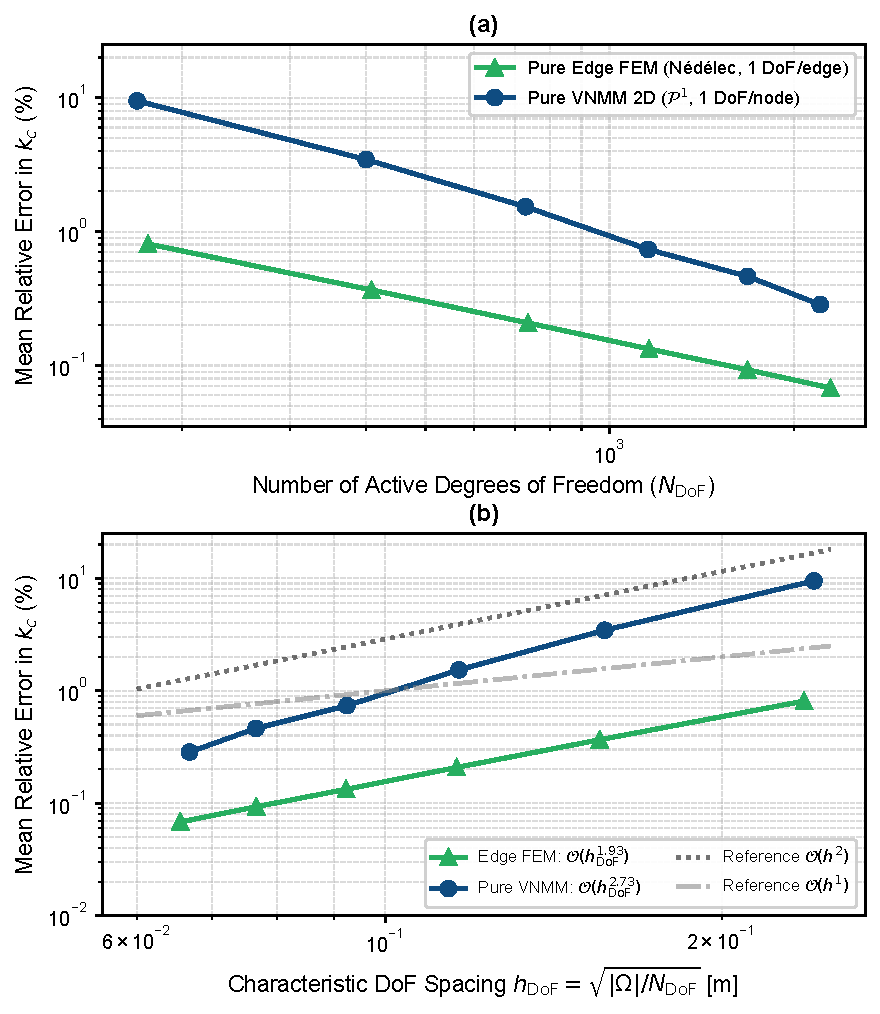
\includegraphics[width=0.62\linewidth]{figura_convergencia_vnmm_vs_fem.pdf}
    \caption{Spectral convergence comparison between Edge FEM and VNMM $\mathcal{P}^1$ for cavity $TE_z$ modes.
        (a) Mean relative error in cutoff wavenumber $k_c$ versus degrees of freedom $N_{\mathrm{DoF}}$;
        (b) Convergence versus characteristic spacing $h_{\mathrm{DoF}}$, showing fitted rates of $\mathcal{O}(h_{\mathrm{DoF}}^{1.93})$ (Edge FEM) and $\mathcal{O}(h_{\mathrm{DoF}}^{2.73})$ (VNMM).}
    \label{fig:convergence_vnmm_fem}
\end{figure}

\subsubsection{Convergence and Accuracy Comparison}
Table~\ref{tab:convergence_6_meshes} and Fig.~\ref{fig:convergence_vnmm_fem} report the convergence history across 6 successive mesh levels ($N \in \{9, 13, 17, 21, 25, 29\}$), together with the Rayleigh error decomposition into pure curl and penalty contributions ($\lambda = \lambda_{\mathrm{curl}} + s_{\mathrm{div}} \lambda_{\mathrm{div}}$) and the irregular cloud performance.

\begin{table}[!htbp]
    \centering
    \small
    \caption{Comparative spectral convergence of resonant wavenumber $k_c$ and error decomposition for cavity $TE_z$ modes across six refinement levels ($s_{\mathrm{div}} = 6.0$, $3 \times 3$ Gauss quadrature): Edge FEM, VNMM $\mathcal{P}^1$ on regular grids (with Rayleigh curl and penalty biases), and VNMM $\mathcal{P}^1$ on irregular clouds ($25\%$ jitter, random directors).}
    \label{tab:convergence_6_meshes}
    \resizebox{\columnwidth}{!}{%
        \begin{tabular}{@{} c c c c cccc c @{}}
            \toprule
            \textbf{Mesh} & $N_{\mathrm{DoF}}$ & $h_{\mathrm{DoF}}$ [m] & \textbf{Edge FEM}   & \multicolumn{4}{c}{\textbf{VNMM $\mathcal{P}^1$ (Regular Grid)}} & \textbf{VNMM $\mathcal{P}^1$ (Irregular)}                                                                                    \\
            \cmidrule(lr){4-4} \cmidrule(lr){5-8} \cmidrule(lr){9-9}
            $N$           &                    &                        & \textbf{Error (\%)} & \textbf{Error $k_c$ (\%)}                                        & \textbf{Error $\lambda$ (\%)}             & \textbf{Curl Bias (\%)} & \textbf{Penalty Bias (\%)} & \textbf{Error $k_c$ (\%)} \\
            \midrule
            9             & 169                & 0.2417                 & 0.810               & 9.484                                                            & 20.16                                     & $-4.78$                 & $+24.94$                   & 24.669                    \\
            13            & 400                & 0.1571                 & 0.367               & 3.454                                                            & 7.08                                      & $+1.29$                 & $+5.79$                    & 11.489                    \\
            17            & 729                & 0.1164                 & 0.208               & 1.534                                                            & 3.10                                      & $+0.66$                 & $+2.44$                    & 5.940                     \\
            21            & 1156               & 0.0924                 & 0.133               & 0.737                                                            & 1.48                                      & $+0.03$                 & $+1.41$                    & 3.102                     \\
            25            & 1681               & 0.0766                 & 0.093               & 0.463                                                            & 0.93                                      & $-0.89$                 & $+1.42$                    & 1.960                     \\
            29            & 2209               & 0.0668                 & 0.068               & 0.285                                                            & 0.57                                      & $-1.14$                 & $+0.64$                    & 1.635                     \\
            \bottomrule
        \end{tabular}%
    }
\end{table}

Key numerical observations include:
\begin{itemize}
    \item \textbf{Monotonicity and Stencil Locality:} Enforcing $|\det(\widehat{\mathbf{A}})| \ge 0.80$ preserves compact nearest-neighbor stencils ($K_{\mathrm{avg}} \approx 6.5$) across all grid levels without parameter tuning, preventing support dilation as $h \to 0$. In tandem with the resolution-matched baseline quadrature ($3 \times 3$ Gauss points), both Edge FEM and VNMM converge monotonically toward the continuum limit.
    \item \textbf{Error Hierarchy and Rates:} Edge FEM delivers lower absolute errors ($0.81\%\text{--}0.07\%$, observed fitted rate $\mathcal{O}(h_{\mathrm{DoF}}^{1.93})$, matching the expected $\mathcal{O}(h^2)$ eigenvalue rate for linear simplicial elements) due to exact circulation cancellation. VNMM displays an observed fitted slope of $\mathcal{O}(h_{\mathrm{DoF}}^{2.73})$ across all levels ($9.48\%\text{--}0.29\%$), steepening to $\mathcal{O}(h_{\mathrm{DoF}}^{2.97})$ on fine grids while operating entirely without topological mesh connectivity. As analyzed below, this super-linear slope is an observed pre-asymptotic effect rather than a claim of higher-order asymptotic accuracy.
\end{itemize}

\paragraph{Pre-Asymptotic Penalty Relief and Rayleigh Decomposition}
The observed fitted slope of $\mathcal{O}(h_{\mathrm{DoF}}^{2.73})$ reflects pre-asymptotic behavior governed by the interaction between curl and divergence penalty operators. As reported in Table~\ref{tab:convergence_6_meshes}, decomposing the discrete Rayleigh quotient into $\lambda = \lambda_{\mathrm{curl}} + s_{\mathrm{div}} \lambda_{\mathrm{div}}$ reveals that on coarse grids ($N=9$), eigenvalue error ($20.16\%$) is dominated by penalty stiffening ($+24.94\%$), with pure curl contributing $-4.78\%$. Under progressive refinement, discrete divergence rapidly vanishes ($\nabla \cdot \vec{E}^h \to 0$), causing the penalty bias to dissipate from $+24.94\%$ down to $+0.64\%$ at $N=29$ ($\approx \mathcal{O}(h_{\mathrm{DoF}}^{2.57})$), while curl discretization error converges monotonically ($-1.14\%$). This confirms that the steep slope represents pre-asymptotic relief of coarse-grid penalty stiffening coupled with dynamic stencil consolidation, narrowing the accuracy gap with Edge FEM from $11.7\times$ to $4.2\times$.

\subsection{Spectral Validation on Irregular Point Clouds with Arbitrary Vector Directors}
\label{subsec:spectral_irregular_clouds}

To evaluate performance under simultaneous spatial and directional disorder, we discretize the cavity across the six refinement levels ($N_{\mathrm{DoF}} \in [169, 2209]$) using the baseline stochastic model (Table~\ref{tab:baseline_computational_setup}), maintaining the baseline quadrature and regularization settings ($3 \times 3$ Gauss points, $s_{\mathrm{div}} = 6.0$, $\widehat{\mathrm{Tol}} = 0.80$).

Table~\ref{tab:convergence_6_meshes} (final column) and Fig.~\ref{fig:convergencia_cavidade_aleatoria} present the convergence history, while Table~\ref{tab:espectro_cavidade_aleatoria_fina} details the first 10 physical modes on the fine cloud ($N_{\mathrm{DoF}} = 2{,}209$).

\begin{figure}[!htbp]
    \centering
    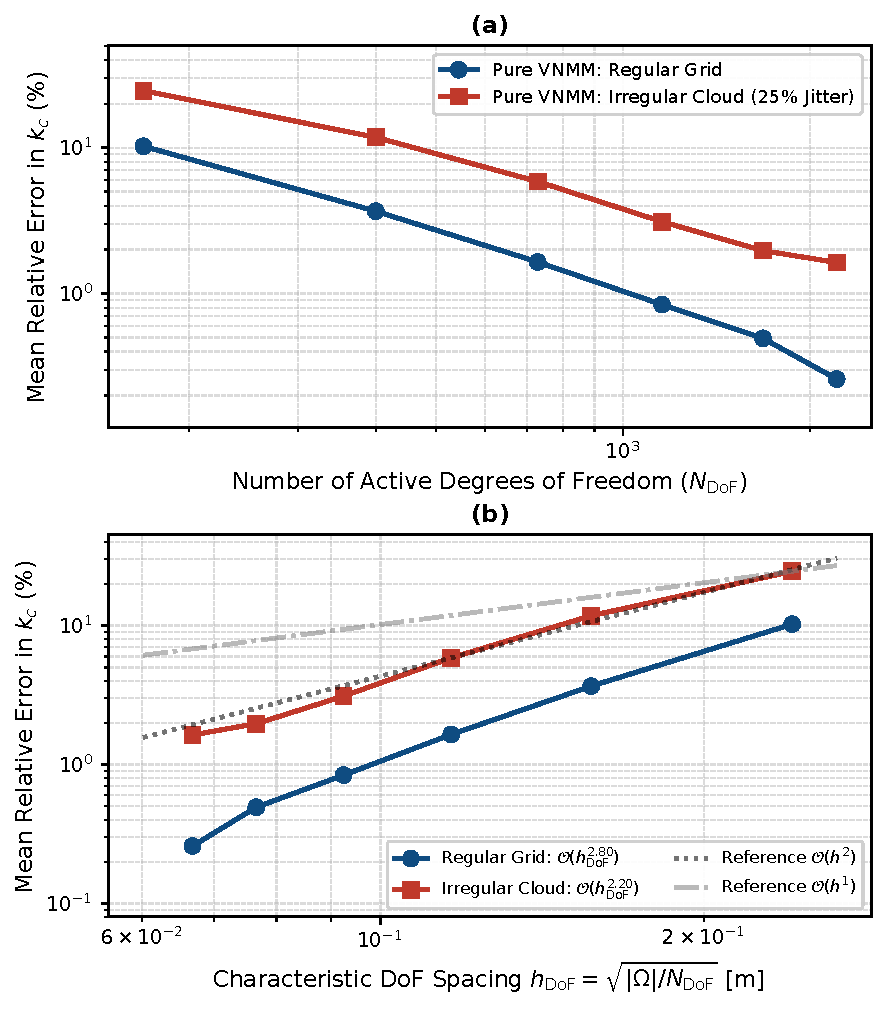
\includegraphics[width=0.62\linewidth]{figura_convergencia_cavidade_aleatoria.pdf}
    \caption{Spectral convergence of VNMM $\mathcal{P}^1$ on regular versus irregular point clouds.
        (a) Mean relative error in cutoff wavenumber $k_c$ versus degrees of freedom $N_{\mathrm{DoF}}$;
        (b) Convergence versus characteristic spacing $h_{\mathrm{DoF}}$, showing fitted slopes of $\mathcal{O}(h_{\mathrm{DoF}}^{2.73})$ (regular grid) and $\mathcal{O}(h_{\mathrm{DoF}}^{2.20})$ (irregular cloud).}
    \label{fig:convergencia_cavidade_aleatoria}
\end{figure}

Critical findings from the irregular cloud campaign include:
\begin{enumerate}
    \item \textbf{Monotonic Convergence under Disorder:} The regularized VNMM converges monotonically with a fitted slope of $\mathcal{O}(h_{\mathrm{DoF}}^{2.20})$, confirming that spatial jitter and random directors do not cause spectral stagnation or locking, consistent with the completeness of $\mathcal{P}^1$.
    \item \textbf{Error Hierarchy and Spectral Purity:} Coarse-mesh errors are elevated compared to regular grids ($24.67\%$ vs. $9.48\%$ at $N=9$) due to loss of Cartesian residual cancellation, but decay smoothly to $1.64\%$ at $N=29$. All 10 lowest computed eigenvalues match analytical physical modes in exact 1-to-1 order, with zero spurious modes detected below $\lambda \le 10$ (Table~\ref{tab:espectro_cavidade_aleatoria_fina}).
    \item \textbf{Support Locality:} Enforcing $|\det(\widehat{\mathbf{A}})| \ge 0.80$ maintains compact candidate queries ($K_{\mathrm{avg}} \in [7.7, 8.2]$, $K_{\max} \le 12$) across all levels, preventing stencil dilation despite severe spatial-directional disorder.
\end{enumerate}

\begin{table}[!htbp]
    \centering
    \small
    \caption{First 10 physical $TE_{nm}$ resonant cavity modes computed on the fine irregular point cloud against analytical references ($2{,}209$ active DoFs).}
    \label{tab:espectro_cavidade_aleatoria_fina}
    \resizebox{\columnwidth}{!}{%
        \begin{tabular}{@{} c c c c c c c @{}}
            \toprule
            \textbf{Mode ($TE_{nm}$)} & $\lambda_{\mathrm{analytical}}$ & $\lambda_{\mathrm{VNMM}}$ & \textbf{Error $\lambda$ (\%)} & $k_{c, \mathrm{analytical}}$ & $k_{c, \mathrm{VNMM}}$ & \textbf{Error $k_c$ (\%)} \\
            \midrule
            $TE_{10}$                 & 1.00                            & 0.9511                    & 4.89\%                        & 1.000                        & 0.975                  & \textbf{2.48\%}           \\
            $TE_{01}$                 & 1.00                            & 0.9544                    & 4.56\%                        & 1.000                        & 0.977                  & \textbf{2.31\%}           \\
            $TE_{11}$                 & 2.00                            & 1.9424                    & 2.88\%                        & 1.414                        & 1.394                  & \textbf{1.45\%}           \\
            $TE_{20}$                 & 4.00                            & 3.9493                    & 1.27\%                        & 2.000                        & 1.987                  & \textbf{0.64\%}           \\
            $TE_{02}$                 & 4.00                            & 3.9930                    & 0.17\%                        & 2.000                        & 1.998                  & \textbf{0.09\%}           \\
            $TE_{21}$                 & 5.00                            & 5.0366                    & 0.73\%                        & 2.236                        & 2.244                  & \textbf{0.37\%}           \\
            $TE_{12}$                 & 5.00                            & 5.1316                    & 2.63\%                        & 2.236                        & 2.265                  & \textbf{1.31\%}           \\
            $TE_{22}$                 & 8.00                            & 8.4144                    & 5.18\%                        & 2.828                        & 2.901                  & \textbf{2.56\%}           \\
            $TE_{30}$                 & 9.00                            & 8.5648                    & 4.84\%                        & 3.000                        & 2.927                  & \textbf{2.45\%}           \\
            $TE_{03}$                 & 9.00                            & 9.4952                    & 5.50\%                        & 3.000                        & 3.081                  & \textbf{2.71\%}           \\
            \midrule
            \textbf{Global Mean}      & ---                             & ---                       & \textbf{3.27\%}               & ---                          & ---                    & \textbf{1.64\%}           \\
            \bottomrule
        \end{tabular}%
    }
\end{table}

% ---------------------------------------------------------
% SUBSECTION 5.7: LIMITATIONS AND SCOPE OF APPLICABILITY
% ---------------------------------------------------------
\subsection{Limitations and Scope of Applicability}
\label{subsec:limitations_scope}

The numerical benchmarks confirm the stability and spectral accuracy of the stabilized VNMM 2D within the investigated canonical configurations. For broader CEM applications, five principal operational boundaries should be considered:
\begin{enumerate}
    \item \textbf{Background Quadrature Scaffolding:} Evaluating the weak form currently relies on background Cartesian integration cells with $3 \times 3$ Gauss quadrature to accommodate intra-cell stencil transitions (Section~\ref{subsubsec:quadrature_sensitivity}). While the Galerkin patch test demonstrated linear completeness for affine vector fields under this integration framework (Section~\ref{subsec:patch_test_galerkin}), incorporating truly cell-free schemes (such as SCNI \cite{chen2001stabilized} or MLPG \cite{atluri2002meshless}) represents an essential step to eliminate background grids in complex domains.

    \item \textbf{Absence of Explicit Tangential-Jump Control:} As analyzed in Section~\ref{subsubsec:tangential_jump_limitations}, the volumetric div-curl penalty acts on discrete divergence and does not directly control tangential trace jumps across shifting support boundaries. While the patch tests, manufactured-solution studies, and cavity benchmarks demonstrate systematic convergence and spectral purity for all tested regular and irregular clouds, stability is established empirically for these regimes rather than as a uniform theoretical guarantee across arbitrary point distributions.

    \item \textbf{Boundary Stencil Starvation and Curvature:} On acute convex corners or curved boundaries, geometric truncation restricts the accessible angular half-space, which may require querying wider candidate neighborhoods ($K > 12$) to satisfy $|\det(\widehat{\mathbf{A}})| \ge \widehat{\mathrm{Tol}}$. Continuous boundary curvature also introduces tangential trace mismatch along curved facets unless boundary directors are adaptively aligned.

    \item \textbf{High-Frequency Dispersion:} In electrically large domains ($kh \gg 1$), numerical dispersion requires dense spatial sampling ($h \le \lambda_{\mathrm{EM}} / 10$), and the div-curl penalty parameter $s_{\mathrm{div}}$ may benefit from frequency-dependent scaling to maintain uniform spectral separation.

    \item \textbf{Material Discontinuities and 3D Extension:} The present formulation focuses on 2D piecewise homogeneous domains. Discontinuous dielectric interfaces ($\epsilon_{r1} \neq \epsilon_{r2}$) require subdomain-partitioned stencils to prevent unphysical gradient smoothing, while 3D formulations require 12-node stencils ($\mathcal{P}_1^3$), increasing local combinatorial search costs.
\end{enumerate}

% =========================================================
% SECTION 6: CONCLUSION AND FUTURE WORKS
% =========================================================
\section{Conclusion and Future Works}
\label{sec:conclusion}

This work established a stabilized Vector Nodal Meshless Method (VNMM 2D) for electromagnetic vector field interpolation and eigenvalue analysis on unstructured point clouds without mesh connectivity. By resolving both local polynomial incompleteness and global variational instabilities, the proposed framework establishes the following core findings:

\subsection{Summary of Findings and Methodological Conclusions}
\label{subsec:summary_conclusions}

\begin{enumerate}
    \item \textbf{Resolution of Local Incompleteness via $\mathcal{P}^1$:}
          Completing the local approximation space ($\mathcal{L}^1 \to \mathcal{P}^1 = \mathcal{P}_1 \times \mathcal{P}_1$) resolves all components of the first-order Jacobian $\nabla \vec{E}^h$, overcoming the $\mathcal{O}(1)$ curl noise floor in pointwise collocation. Furthermore, $\mathcal{P}^1$ unconditionally passes the Galerkin patch test to machine precision ($\le 7.38 \times 10^{-14}$) for all seven affine modes---confirming linear completeness of the discrete Galerkin operator---and achieves systematic numerical convergence (with fitted rates of $\mathcal{O}(h^{2.08})$ in $L^2$ and $\mathcal{O}(h^{0.75})$ in $H(\mathbf{curl})$ across the tested refinement sequences) in the Galerkin Method of Manufactured Solutions (MMS), whereas the incomplete $\mathcal{L}^1$ basis exhibits variational breakdown ($15\%\text{--}47\%$ error) and convergence stagnation.

    \item \textbf{Scale-Invariant Support Selection ($\widehat{\mathbf{A}} + \text{$k$-d tree}$):}
          Formulating support qualification via the dimensionless placement matrix $\widehat{\mathbf{A}}$ removes the quartic scaling $\mathcal{O}(h^4)$, decoupling stencil geometry from absolute grid refinement. Enforcing $|\det(\widehat{\mathbf{A}})| \ge \widehat{\mathrm{Tol}}$ together with early-stopping $k$-d tree search preserves compact stencils ($K_{\mathrm{avg}} \approx 6.5\text{--}11$) down to fine resolutions and bounds local conditioning ($\kappa_2(\widehat{\mathbf{A}}) \le 5.9$) under $25\%$ spatial disorder.

    \item \textbf{Delineation of Topological Conformity vs. Mesh-Free Non-Conformity:}
          The formal proof of the Local Dual Equivalence Theorem (\ref{app:dual_whitney_proof}) establishes that VNMM reproduces lowest-order Whitney edge elements on conforming simplices down to machine precision ($\approx 10^{-16}$). On arbitrary clouds, moving support stencils destroy global trace continuity ($V_h \not\subset H(\mathbf{curl}; \Omega)$) and discrete de Rham sequence exactness, causing gradient nullspace leakage in unregularized curl-curl formulations.

    \item \textbf{Variational Div-Curl Regularization and Baseline Spectral Accuracy:}
          Volumetric div-curl regularization provides effective spurious mode shifting without expanding system dimensions or introducing auxiliary multipliers. On the 361-DoF base resonant cavity under the resolution-matched baseline quadrature ($20 \times 20$ cells, $3 \times 3$ Gauss points), the stabilized formulation achieves a global mean cutoff wavenumber error of $4.01\%$ (spanning $0.41\%\text{--}7.33\%$ across the first ten physical resonances). In the calibrated penalty window ($s_{\mathrm{div}} \in [6.0, 10.0]$), spurious gradient modes are shifted completely beyond the operational spectrum ($\lambda_{\mathrm{spur}} = 11.84 > 10.37$) while physical resonances incur minimal penalty distortion ($R_{\mathrm{div}} \le 1.65\%$). Multi-level refinement studies yield observed fitted convergence rates of $\mathcal{O}(h_{\mathrm{DoF}}^{2.73})$ on regular lattices and $\mathcal{O}(h_{\mathrm{DoF}}^{2.20})$ under stochastic perturbations across the investigated discretization levels.

    \item \textbf{Quadrature Transparency: Resolution-Matched Integration vs. Under-Integration Deception:}
          Systematic sensitivity analysis across background cell densities and Gauss rules (Table~\ref{tab:quadrature_sensitivity}) serves as a cautionary pedagogical case study for non-conforming meshless methods. It reveals that the apparent low error of $1.09\%$ obtained under coarse under-integration ($10 \times 10$ cells with $2 \times 2$ Gauss points) is a deceptive numerical artifact arising from error cancellation between discrete curl softening across intra-cell stencil boundaries and penalty stiffening, while concealing a $140$-dimensional spurious rank deficiency in $\mathbf{K}_{\mathrm{curl}}$. Eliminating this artificial softening through dense, resolution-matched quadrature ($N_g / N_{\mathrm{DoF}} \approx 10$, $\dim\ker(\mathbf{K}_{\mathrm{curl}}) = 0$) restores full numerical rank and establishes a consistent baseline spatial discretization error of $4.01\%$, ensuring that observed convergence rates reflect genuine vector polynomial approximation rather than under-integration artifacts.

    \item \textbf{Operational Scope and Methodological Caveats:}
          While the stabilized VNMM demonstrates spectral purity and systematic convergence across all tested configurations, its operational scope entails three principal caveats established in Section~\ref{subsec:limitations_scope}: (i) evaluation of weak forms currently relies on a background Cartesian integration grid---requiring a dense ratio ($N_g / N_{\mathrm{DoF}} \approx 10$) to sufficiently integrate intra-cell stencil transitions---highlighting the importance of developing truly cell-free schemes (e.g., SCNI or MLPG); (ii) the volumetric div-curl penalty acts on discrete divergence rather than directly penalizing tangential trace jumps $[\hat{n} \times \vec{E}^h]$ across shifting support boundaries, meaning that stability is verified empirically for the tested regimes rather than guaranteed uniformly via a priori error bounds; and (iii) the present scope is restricted to 2D piecewise homogeneous domains at low-to-moderate electrical size, with material interfaces, curved-boundary director alignment, and 3D extensions ($\mathcal{P}_1^3$) forming natural targets for future investigation.
\end{enumerate}

\subsection{Promising Directions for Future Research}
\label{subsec:future_works}

Building upon this 2D stabilized vector formulation, key avenues for future investigation include:
\begin{enumerate}
    \item \textbf{3D Vector Formulations:} Extending the complete basis to 3D ($\mathcal{P}_1^3$, $M_{\mathrm{supp}} = 12$) for 3D resonant cavities, waveguiding structures, and radiation problems \cite{goncalves2023vector}.
    \item \textbf{Explicit Tangential-Jump Stabilization and Rigorous Error Bounds:} Developing explicit interface jump penalty terms---drawing on Interior Penalty (IP) and Discontinuous Galerkin (DG) formulations for Maxwell operators \cite{houston2004mixed, hesthaven2004high, nguyen2011hybridizable}---to penalize tangential discontinuities $[\hat{n} \times \vec{E}^h]$ across shifting support transitions, paving the way for a priori error estimates and provable uniform stability on arbitrary point clouds.
    \item \textbf{Cell-Free Quadrature and Complex Boundaries:} Replacing background integration cells with cell-free schemes (SCNI \cite{chen2001stabilized} or MLPG \cite{atluri2002meshless}) to eliminate quadrature scaffolding and accommodate moving or curved boundaries.
    \item \textbf{Multi-Seed Statistical Characterization:} Conducting Monte Carlo campaigns across multiple random cloud realizations to evaluate statistical error distributions and qualification success rates.
    \item \textbf{Material Interfaces:} Developing multi-tree spatial data structures \cite{parreira2006efficient} to restrict stencils to homogeneous subdomains, preserving constitutive jumps ($\epsilon_{r1} \neq \epsilon_{r2}$) and enforcing normal flux continuity across discontinuities.
    \item \textbf{Hybrid EFEM--VNMM Coupling and Electrical Machines:} Coupling canonical Edge FEM in structured regions with VNMM in geometrically complex zones or narrow moving air gaps (e.g., in rotating electrical machinery \cite{coppoli2012induction}), leveraging the constructive Whitney equivalence for seamless interface continuity without remeshing or sliding-mesh interpolation artifacts.
\end{enumerate}


\appendix

\section{Formal Proof of the Local Constructive Equivalence Theorem}
\label{app:dual_whitney_proof}

This appendix provides the complete constructive proof of Theorem~\ref{thm:dual_equivalence} (Local Constructive Equivalence under Conforming Midpoint/Tangent Placement between the VNMM $\mathcal{L}^1$ basis and lowest-order Whitney 1-forms on triangular simplices).

\begin{proof}
    The proof proceeds in five constructive steps:

    \textbf{Step 1: Identity of Local Vector Polynomial Spaces.}
    The lowest-order Whitney space $\mathcal{W}(T)$ on $T$ is spanned by fields of the form $[a_1 + \alpha y, a_2 - \alpha x]^T$. By inspection, $\mathcal{W}(T) \equiv \mathcal{L}^1 = \operatorname{span}\{[1,0]^T, [0,1]^T, [y,-x]^T\}$, so both formulations span the same 3-dimensional vector polynomial space.

    \textbf{Step 2: Constancy of Tangential Field Projection Along Simplex Edges.}
    Let $\vec{u}(\mathbf{x}) = [a_1 + \alpha y, a_2 - \alpha x]^T \in \mathcal{L}^1$. The directional projection of $\vec{u}(\mathbf{x})$ along unit director $\vec{t}_k = [\Delta x_k / L_k, \Delta y_k / L_k]^T$ is:
    \begin{equation}
        \vec{u}(\mathbf{x}) \cdot \vec{t}_k = \frac{1}{L_k} \left[ a_1 \Delta x_k + a_2 \Delta y_k + \alpha (y \Delta x_k - x \Delta y_k) \right].
    \end{equation}
    Since any point $\mathbf{x} = (x,y)$ on edge $e_k$ satisfies $(x - x_k)\Delta y_k - (y - y_k)\Delta x_k = 0$, the rotational term $y \Delta x_k - x \Delta y_k = y_k \Delta x_k - x_k \Delta y_k$ is constant along the entire edge length. Therefore, the tangential projection is invariant along $e_k$:
    \begin{equation}
        \vec{u}(\mathbf{x}) \cdot \vec{t}_k = \vec{u}(M_k) \cdot \vec{t}_k, \quad \forall \mathbf{x} \in e_k.
        \label{eq:edge_constancy_app}
    \end{equation}

    \textbf{Step 3: Reduction of Edge Circulation to Pointwise Midpoint Value.}
    Using Eq.~\eqref{eq:edge_constancy_app}, the line integral defining the FEM circulation degree of freedom along edge $e_j$ simplifies to:
    \begin{equation}
        \oint_{e_j} \vec{u} \cdot d\boldsymbol{\ell} = \int_{-L_j/2}^{L_j/2} \left( \vec{u}(\mathbf{x}(s)) \cdot \vec{t}_j \right) ds = \left( \vec{u}(M_j) \cdot \vec{t}_j \right) \int_{-L_j/2}^{L_j/2} ds = L_j \left( \vec{u}(M_j) \cdot \vec{t}_j \right).
    \end{equation}
    Substituting the $k$-th Whitney basis function $\vec{w}_k \in \mathcal{W}(T)$, which satisfies $\oint_{e_j} \vec{w}_k \cdot d\boldsymbol{\ell} = \delta_{jk}$ by construction, yields:
    \begin{equation}
        L_j \left( \vec{w}_k(M_j) \cdot \vec{t}_j \right) = \delta_{jk} \quad \implies \quad \left( L_k \vec{w}_k(M_j) \right) \cdot \vec{t}_j = \delta_{jk}.
        \label{eq:whitney_midpoint_proj_app}
    \end{equation}

    \textbf{Step 4: Uniqueness and Exact Identification with VNMM Shape Functions.}
    By definition of the VNMM 2D $\mathcal{L}^1$ interpolation problem on the support triad $\{M_j, \vec{t}_j\}_{j=1}^3$, the shape functions satisfy $\vec{N}_k(M_j) \cdot \vec{t}_j = \delta_{jk}$. Consider the difference field:
    \begin{equation}
        \vec{d}_k(\mathbf{x}) = \vec{N}_k(\mathbf{x}) - L_k \vec{w}_k(\mathbf{x}) \in \mathcal{L}^1.
    \end{equation}
    Evaluating its projection at each midpoint $M_j$:
    \begin{equation}
        \vec{d}_k(M_j) \cdot \vec{t}_j = \vec{N}_k(M_j) \cdot \vec{t}_j - L_k \left( \vec{w}_k(M_j) \cdot \vec{t}_j \right) = \delta_{jk} - \delta_{jk} = 0, \quad \forall j \in \{1, 2, 3\}.
    \end{equation}
    By Steps 2--3, $\vec{d}_k$ has zero circulation along every edge, and edge circulations are unisolvent on $\mathcal{W}(T)=\mathcal{L}^1$ for non-degenerate $T$; hence $\vec{d}_k \equiv \mathbf{0}$ (equivalently, the local moment placement matrix $\mathbf{A} \in \mathbb{R}^{3 \times 3}$ is non-singular with $\det \mathbf{A} \neq 0$), which proves the exact identity $\vec{N}_k(\mathbf{x}) \equiv L_k \vec{w}_k(\mathbf{x})$ everywhere in $\mathbb{R}^2$.

    \textbf{Step 5: Verification of Differential Invariants.}
    1. \textit{Divergence:} For any field $\vec{u} = [a_1 + \alpha y, a_2 - \alpha x]^T \in \mathcal{L}^1$, we have $\nabla \cdot \vec{u} = \partial(a_1 + \alpha y)/\partial x + \partial(a_2 - \alpha x)/\partial y \equiv 0$. Thus, $\nabla \cdot \vec{w}_k \equiv 0$ and $\nabla \cdot \vec{N}_k \equiv 0$ everywhere.
    2. \textit{Curl:} Applying Stokes' theorem over triangle $T$ for Whitney 1-form $\vec{w}_k$:
    \begin{equation}
        \int_T (\nabla \times \vec{w}_k)_z d\Omega = \oint_{\partial T} \vec{w}_k \cdot d\boldsymbol{\ell} = \sum_{j=1}^3 \delta_{jk} = 1 \implies (\nabla \times \vec{w}_k)_z = \frac{1}{|T|}.
    \end{equation}
    By the identity proved in step 4, $(\nabla \times \vec{N}_k)_z = L_k (\nabla \times \vec{w}_k)_z = L_k / |T|$.
\end{proof}

\section{Derivation of the Derivative Aliasing Scaling in the Incomplete Basis}
\label{app:heuristic_aliasing_proof}

This appendix details the order-of-magnitude scaling derivation supporting Heuristic~\ref{heur:L1_aliasing}.

\begin{proof}[Derivation of Scaling Estimate]
    Let any discrete vector field $\vec{E}^h \in \mathcal{L}^1$ be expanded in terms of the solenoidal basis:
    \begin{equation}
        \vec{E}^h(x, y) = a \begin{bmatrix} 1 \\ 0 \end{bmatrix} + b \begin{bmatrix} 0 \\ 1 \end{bmatrix} + c \begin{bmatrix} y \\ -x \end{bmatrix}, \quad a, b, c \in \mathbb{R}.
    \end{equation}
    Direct differentiation with respect to spatial coordinates yields the discrete Jacobian tensor:
    \begin{equation}
        \mathbf{J}^h = \begin{bmatrix}
            \frac{\partial E_x^h}{\partial x} & \frac{\partial E_x^h}{\partial y} \\[4pt]
            \frac{\partial E_y^h}{\partial x} & \frac{\partial E_y^h}{\partial y}
        \end{bmatrix} = \begin{bmatrix}
            0  & c \\
            -c & 0
        \end{bmatrix}.
    \end{equation}
    Inspection shows that $\partial E_x^h/\partial x \equiv 0$, $\partial E_y^h/\partial y \equiv 0$, and $\partial E_x^h/\partial y + \partial E_y^h/\partial x = c - c \equiv 0$, identically satisfying the linear constraints in Eq.~\eqref{eq:L1_derivative_constraints}.

    Now consider a general smooth physical field $\vec{E} \in [C^2(\Omega)]^2$. Its Taylor expansion centered at evaluation point $P$ is $\vec{E}(\mathbf{x}) = \vec{E}(P) + \mathbf{J}(P) \Delta\mathbf{x} + \mathcal{O}(h^2)$, where $\mathbf{J}(P)$ has non-zero diagonal entries ($\partial E_x/\partial x \neq 0$ or $\partial E_y/\partial y \neq 0$). Collocating $\vec{E}^h$ at support nodes $\mathbf{x}_k$ ($k=1,2,3$) along unit directors $\vec{t}_k$ defines the linear placement system $\mathbf{A} [a, b, c]^T = \mathbf{e}$, where $e_k = \vec{E}(\mathbf{x}_k) \cdot \vec{t}_k$.

    Subtracting the projection of the unrepresented linear components $(\mathbf{J}(P) - \mathbf{J}^h) \Delta\mathbf{x}_k \cdot \vec{t}_k$ yields a nodal projection residual $\mathbf{r} \in \mathbb{R}^3$ with asymptotic magnitude $\|\mathbf{r}\| \sim \mathcal{O}(h)$. In the $3 \times 3$ moment placement matrix $\mathbf{A}$ (Eq.~\eqref{eq:matrix_A_L1}), translation columns 1--2 scale as $\mathcal{O}(1)$, while the rotational moment column 3 scales as $(\Delta y_k t_{kx} - \Delta x_k t_{ky}) \sim \mathcal{O}(h)$. Consequently, by Cramer's rule or Neumann inversion, the third row of $\mathbf{A}^{-1}$ (which maps nodal data to the rotational DoF $c = -\frac{1}{2}(\nabla \times \vec{E}^h)_z$) scales as $\|\operatorname{Row}_3(\mathbf{A}^{-1})\| \sim \mathcal{O}(h^{-1})$.

    The numerical error in the reconstructed curl at evaluation point $P$ is therefore governed by the propagation of the projection remainder:
    \begin{equation}
        \begin{aligned}
            |(\nabla \times \vec{E})_z - (\nabla \times \vec{E}^h)_z| & = 2 |c_{\mathrm{exact}} - c|                                                                                               \\
                                                                      & \sim \|\operatorname{Row}_3(\mathbf{A}^{-1})\| \|\mathbf{r}\| = \mathcal{O}(h^{-1}) \cdot \mathcal{O}(h) = \mathcal{O}(1),
        \end{aligned}
    \end{equation}
    which is asymptotically independent of $h$ and generates an $\mathcal{O}(1)$ error plateau under spatial refinement ($h \to 0$) in the collocated setting for generic node/director placements (see Remark~\ref{rem:heur1_scope}).
\end{proof}


\section*{CRediT Authorship Contribution Statement}
\textbf{Renato C. Mesquita}: Conceptualization, Methodology, Software, Formal analysis, Investigation, Writing -- original draft, Writing -- review \& editing, Visualization, Supervision, Funding acquisition.
\textbf{Elson J. da Silva}: Conceptualization, Formal analysis, Writing -- review \& editing.
\textbf{Bárbara M. F. Gonçalves}: Methodology, Software, Validation, Investigation, Formal analysis, Writing -- review \& editing.
\textbf{Luilly A. G. Ortiz}: Methodology, Software, Validation, Data curation, Writing -- review \& editing.

\section*{Declaration of Competing Interest}
The authors declare that they have no known competing financial interests or personal relationships that could have appeared to influence the work reported in this paper.

\section*{Data Availability}
The simulation scripts, benchmark datasets, and point-cloud generation algorithms supporting the findings of this study are available from the corresponding author upon reasonable request.

% --- AGRADECIMENTOS ---
\section*{Acknowledgements}
The authors would like to thank the Brazilian research funding agencies CAPES, CNPq, and FAPEMIG for their financial support during the development of this research project.

\section*{Declaration of Generative AI and AI-Assisted Technologies in the Writing Process}
During the preparation of this work, the authors used Google Antigravity / Gemini in order to assist with English language editing, LaTeX code formatting, script automation for numerical data consistency, and cross-referencing verification. After using this tool, the authors carefully reviewed, verified, and edited all resulting content and take full responsibility for the integrity and accuracy of the publication.

% --- REFERÊNCIAS BIBLIOGRÁFICAS ---
\bibliographystyle{elsarticle-num}
\bibliography{references}

\end{document}

\endinput
%%
%% End of file `elsarticle-template-num.tex'.